
%----------------------------------------------------------------------------------------
%	PACKAGES AND THEMES
%----------------------------------------------------------------------------------------

\documentclass{beamer}
\usepackage[brazil]{babel}
\mode<presentation> {

% The Beamer class comes with a number of default slide themes
% which change the colors and layouts of slides. Below this is a list
% of all the themes, uncomment each in turn to see what they look like.

%\usetheme{default}
%\usetheme{AnnArbor}
%\usetheme{Antibes}
%\usetheme{Bergen}
%\usetheme{Berkeley}
%%\usetheme{Berlin}
%%\usetheme{Boadilla}
%%%\usetheme{CambridgeUS}
%\usetheme{Copenhagen}
%\usetheme{Darmstadt}
%\usetheme{Dresden}
\usetheme{Frankfurt}
%\usetheme{Goettingen}
%\usetheme{Hannover}
%%\usetheme{Ilmenau}
%\usetheme{JuanLesPins}
%\usetheme{Luebeck}
%\usetheme{Madrid}
%\usetheme{Malmoe}
%\usetheme{Marburg}
%\usetheme{Montpellier}
%\usetheme{PaloAlto}
%%\usetheme{Pittsburgh}
%\usetheme{Rochester}
%\usetheme{Singapore}
%\usetheme{Szeged}
%\usetheme{Warsaw}

% As well as themes, the Beamer class has a number of color themes
% for any slide theme. Uncomment each of these in turn to see how it
% changes the colors of your current slide theme.

%\usecolortheme{albatross}
%\usecolortheme{beaver}
%\usecolortheme{beetle}
%\usecolortheme{crane}
%\usecolortheme{dolphin}
%\usecolortheme{dove}
%\usecolortheme{fly}
%\usecolortheme{lily}
%\usecolortheme{orchid}
%\usecolortheme{rose}
%\usecolortheme{seagull}
%\usecolortheme{seahorse}
%\usecolortheme{whale}
%\usecolortheme{wolverine}

%\setbeamertemplate{footline} % To remove the footer line in all slides uncomment this line
\setbeamertemplate{footline}[page number] % To replace the footer line in all slides with a simple slide count uncomment this line



% pra que serve?
%\setbeamercovered{transparent}

\setbeamertemplate{navigation symbols}{} % To remove the navigation symbols from the bottom of all slides uncomment this line
}

\usepackage{graphicx} % Allows including images
\usepackage{booktabs} % Allows the use of \toprule, \midrule and \bottomrule in tables


% ---
% Pacotes básicos 
% ---
\usepackage{lmodern}			% Usa a fonte Latin Modern			
\usepackage[T1]{fontenc}		% Selecao de codigos de fonte.
\usepackage[utf8]{inputenc}		% Codificacao do documento (conversão automática dos acentos)
\usepackage{color}				% Controle das cores
\usepackage{microtype} 			% para melhorias de justificação
% ---
		
% ---
% Pacotes de citações
% ---
% Paginas com as citações na bibl
\usepackage[alf]{abntex2cite}	% Citações padrão ABNT

% --- 
% CONFIGURAÇÕES DE PACOTES
% --- 
\usepackage{amsmath}
\usepackage{multirow}
% helvetica no titulo dos capitulos
%\usepackage[scaled]{helvet}
\usepackage{tgheros}
%real numbers
\usepackage{amssymb}
%\hyphenation{Recomendação}

\DeclareMathOperator*{\argmax}{arg\,max}
% alterando o aspecto da cor azul
\definecolor{blue}{RGB}{41,5,195}


%% sumario com algarismos romanos
%\defbeamertemplate{subsection in toc}{bullets}{%
  %\leavevmode
  %\parbox[t]{1em}{\textbullet\hfill}%
  %\parbox[t]{\dimexpr\textwidth-1em\relax}{\inserttocsubsection}\par}
%\defbeamertemplate{section in toc}{sections numbered roman}{%
  %\leavevmode%
  %\MakeUppercase{\romannumeral\inserttocsectionnumber}.\ %
  %\inserttocsection\par}
%\setbeamertemplate{section in toc}[sections numbered roman]
%\setbeamertemplate{subsection in toc}[bullets]


%% fonte
    %\usefonttheme{structurebold}

    \setbeamerfont{title}{series=\bfseries,parent=structure}
    \setbeamerfont{subtitle}{size=\scriptsize,series=\bfseries,parent=structure}
    \setbeamerfont{author}{size=\scriptsize,series=\bfseries,parent=structure}
    \setbeamerfont{institute}{size=\scriptsize,series=\bfseries,parent=structure}
    \setbeamerfont{date}{size=\scriptsize,series=\bfseries,parent=structure}

%\hyphenation{corretamente}

%----------------------------------------------------------------------------------------
%	TITLE PAGE
%----------------------------------------------------------------------------------------

%\title[Short title]{Full Title of the Talk} % The short title appears at the bottom of every slide, the full title is only on the title page
\title[Sistema de Recomendação]{\textsc{Desenvolvimento de uma Biblioteca Computacional para Sistemas de Recomendação de Lojas de Comércio Online}} 

%\author[Antônio Viggiano, Fernando Fochi]{Antônio Viggiano, Fernando Fochi}

\institute[USP] % Your institution as it will appear on the bottom of every slide, may be shorthand to save space
{
\\[-1cm]


\includegraphics[width=0.2\textwidth]{../img/logo_poli} \\

Escola Politécnica da Universidade de São Paulo \\[0.5cm]

\begin{minipage}[t]{0.35\textwidth}
\begin{center}
Antônio Viggiano \\
\texttt{agfviggiano@gmail.com}
\end{center}
\end{minipage}
\begin{minipage}[t]{0.35\textwidth}
\begin{center}
Fernando Fochi \\
\texttt{fernando.fochi@gmail.com}
\end{center}
\end{minipage}

\vspace{0.5cm}
Prof. Dr. Fábio Gagliardi Cozman
}
\date{\today} % Date, can be changed to a custom date


% remover icones de bibliografia
\setbeamertemplate{bibliography item}[triangle]

%bibliography sem paginas
\usepackage{appendixnumberbeamer}

%numero em tabelas etc
\setbeamertemplate{caption}[numbered]

%espaco entre caption
%\usepackage{caption}
%\captionsetup{skip=0pt,belowskip=0pt}
\newcommand\numbered{\setbeamertemplate{footline}{%
  \raisebox{5pt}{\makebox[\paperwidth]{%
    \hfill\makebox[10pt]{%
      \scriptsize\insertframenumber}}}}}

\newcommand\unnumbered{\setbeamertemplate{footline}{}\addtocounter{framenumber}{-1}}


\begin{document}
%!TEX root = index.tex
%----------------------------------------------------------------------------------------
%	TITLE PAGE
%----------------------------------------------------------------------------------------

%\title[Short title]{Full Title of the Talk} % The short title appears at the bottom of every slide, the full title is only on the title page
\title[Sistema de Recomendação]{\rmfamily Desenvolvimento de um Sistema de Recomendação para e-Commerces} 


\author{Antônio Viggiano, Fernando Fochi} % Your name
\institute[USP] % Your institution as it will appear on the bottom of every slide, may be shorthand to save space
{
Escola Politécnica da Universidade de São Paulo \\ % Your institution for the title page
\medskip
\texttt{agfviggiano@gmail.com, fernando.fochi@gmail.com} % Your email address
}
\date{\today} % Date, can be changed to a custom date

\begin{document}

\begin{frame}
\titlepage % Print the title page as the first slide
\end{frame}


%!TEX root = index.tex
\begin{frame}
\frametitle{Sumário} % Table of contents slide, comment this block out to remove it
\tableofcontents % Throughout your presentation, if you choose to use \section{} and \subsection{} commands, these will automatically be printed on this slide as an overview of your presentation
\end{frame}
%!TEX root = index.tex
\section[Introdução]{Introdução}


\begin{frame}{Introdução}{Importância econômica}
\begin{columns}[b] % The "c" option specifies centered vertical alignment while the "t" option is used for top vertical alignment

\column{.5\textwidth} % 

\begin{figure}[ht]
    \begin{center}
    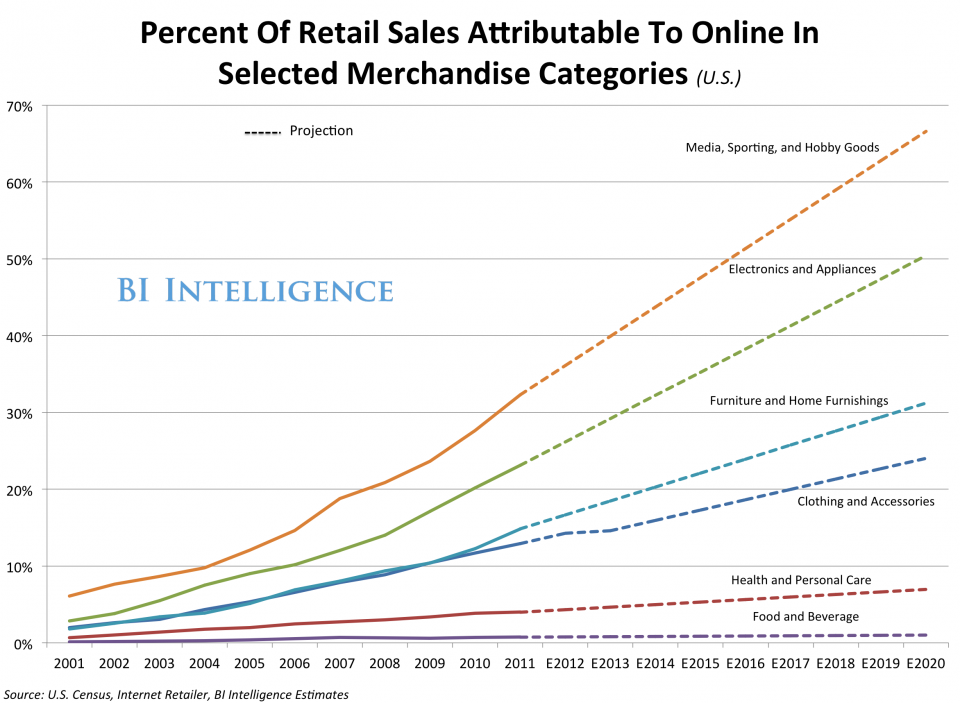
\includegraphics[width=1\textwidth]{img/crescimento-ecommerce}\caption{Percentual de vendas de varejo atribuídas a lojas online nos EUA por categoria \cite{crescimento-ecommerce}}
    \end{center}
\end{figure}

\column{.5\textwidth} %
\begin{figure}[ht]
    \begin{center}
    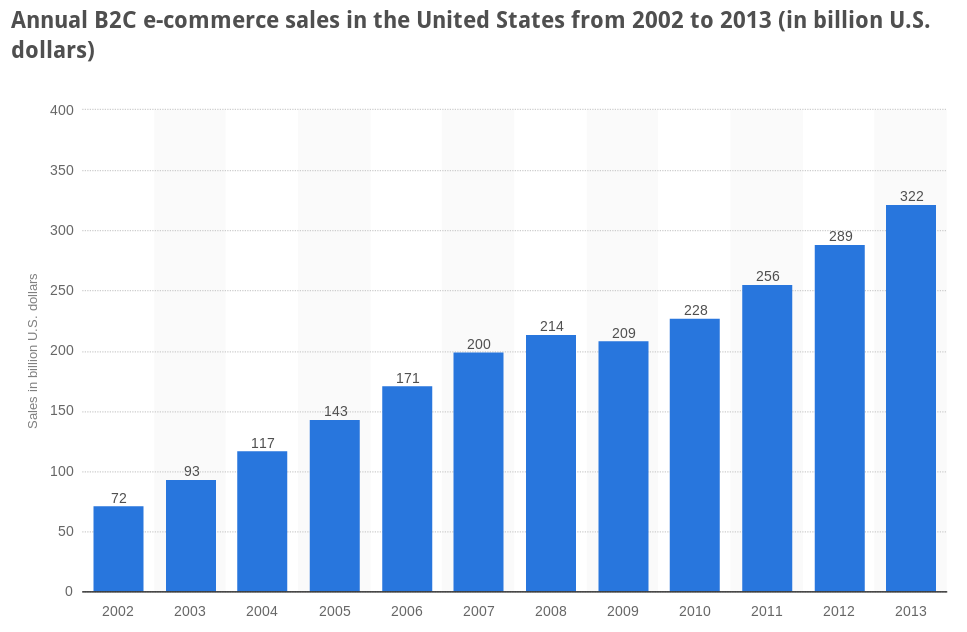
\includegraphics[width=1\textwidth]{img/sales-ecommerce}\caption{Vendas de varejo atribuídas a lojas online nos EUA \cite{sales-ecommerce}}
    \end{center}
\end{figure}

\end{columns}

\end{frame}


\begin{frame}{Introdução}{Aplicação}
\begin{columns}[c]

\column{.5\textwidth} % Left column and width

\begin{figure}[ht]
    \begin{center}
    
\includegraphics[height=30px]{img/facebook}

    Relações de amizade
    \end{center}
\end{figure}

\column{.5\textwidth} % Right column and width

\begin{figure}[ht]
    \begin{center}
    \includegraphics[height=30px]{img/lastfm}

    Músicas
    \end{center}
\end{figure}
\end{columns}
\begin{columns}[b]

\column{.3333\textwidth}

\begin{figure}[ht]
    \begin{center}
    
\includegraphics[height=30px]{img/amazon}

    Livros \textbf{35 \%} \\
    \cite{amazon35}
    \end{center}
\end{figure}

\column{.3333\textwidth}
\begin{figure}[ht]
    \begin{center}
    
\includegraphics[height=23px]{img/google-news}

    Notícias \textbf{38 \%} \\
    \cite{das2007google}
    \end{center}
\end{figure}

\column{.3333\textwidth}
\begin{figure}[ht]
    \begin{center}
    \includegraphics[height=30px]{img/netflix}

    Filmes \textbf{75 \%} \\
    \cite{netflix75}
    \end{center}
\end{figure}
\end{columns}
\end{frame}




\begin{frame}{Introdução}{O que são Sistemas de Recomendação?}
\begin{block}{Definição}
``São ferramentas e técnicas de software destinadas a prover sugestões de itens para usuários'' \cite{ricci2011introduction-chap1}
\end{block}

\begin{block}{Etapas principais}
\begin{itemize}
    \item Aquisição dos dados de entrada
    \item Determinação das recomendações
    \item Apresentação dos resultados ao usuário
\end{itemize}
\end{block}
\end{frame}
%!TEX root = index.tex
\chapter[Objetivos]{Objetivos}
\label{chap:objetivos}

O objetivo do presente Trabalho de Conclusão de Curso é o desenvolvimento de um Sistema de Recomendação de produtos para e-commerces, e respectiva análise de desempenho das recomendações propostas. 

Serão propostos quatro diferentes algoritmos de recomendação, e será feita uma avaliação comparativa entre eles. A explicação detalhada dos métodos se encontra no Capítulo \ref{chap:sintese_de_solucoes}.

Essa ferramenta tem como finalidade a automatização do processo de sugestão de itens, e pode ser aplicada em diversas áreas da indústria, tais como na indicação de notícias, músicas, relações de amizade ou artigos científicos. No nosso trabalho, o sistema terá como foco a sugestão de produtos de lojas de comércio online que disponham de um histórico de compras dos usuários e das características dos produtos.

A qualidade das recomendações será avaliada quanto a precisão e abrangência. Para os métodos em que se possui uma medida de similaridade entre produtos, será avaliada a distância entre os itens efetivamente comprados pelo cliente e aqueles previstos pelo sistema. Uma descrição detalhada da avaliação do sistema de recomendação está descrita no Capítulo \ref{cha:avalia_o_de_desempenho}.

Por meio de uma validação cruzada, analisaremos a influência dos principais parâmetros do problema na qualidade das recomendações, como o tamanho do banco de dados ou a quantidade de informações de itens e clientes utilizadas na recomendação.

Será discutido o impacto dos principais desafios tecnológicos e científicos dos sistemas de recomendação na nossa proposta de solução, tais como a escalabilidade, a adaptação a novos usuários e a esparsidade dos dados \cite{sarwar2000analysis}.

Ao final, será possível extrair uma validação experimental das diretrizes fundamentais a serem seguidas por e-commerces que desejem desenvolver um sistema de recomendação próprio ou que queiram utilizar o sistema desenvolvido neste trabalho. 
%!TEX root = index.tex
\section[Estado da Arte]{Estado da Arte}
\subsection{Estado da arte dos problemas} % (fold)
\label{sub:estado_da_arte_dos_problemas}
% subsection estado_da_arte_dos_problemas (end)
\begin{frame}
\frametitle{Estado da Arte}
\begin{itemize}
	\item $\mathcal{U}$ conjunto de todos os usuários $u$ com características $c$
	\item $\mathcal{I}$ conjunto de todos os itens $i$ com atributos $f$
	\item $r_{ui}$ o histórico avaliações dos itens $i$ pelos usuários $u$\par{~}
	\item $\ell$ função de utilidade 
	\begin{itemize}
		\item $\ell: \mathcal{U} \times \mathcal{I} \rightarrow \mathcal{R}$
		\item $\mathcal{R}$ conjunto totalmente ordenado, p.ex. $\left\{-1, 0, +1\right\}$ ou $[1, 5]$
	\end{itemize}
\end{itemize}


\begin{block}{Objetivo}
Determinar o item $\tilde{\imath}_u$ que maximize a utilidade $\ell_{ui}$ do usuário $u$:
\end{block}

\begin{equation} 
\label{eq:utilidade}
\forall u \in \mathcal{U}, ~ \tilde{\imath}_u = \argmax_{i \in \mathcal{I}}{\ell_{ui}}
\end{equation}

\end{frame}


%% TODO trocar por animacao
\begin{frame}
\frametitle{Estado da Arte}
\begin{block}{Objetivo}
Determinar o item $\tilde{\imath}_u$ que maximize a utilidade $\ell_{ui}$ do usuário $u$:
\end{block}

$$
\forall u \in \mathcal{U}, ~ \tilde{\imath}_u = \argmax_{i \in \mathcal{I}}{\ell_{ui}}
$$


\begin{alertblock}{Problema}
$\ell$ desconhecida
\end{alertblock}

\begin{itemize}
	\item Em algumas formulações se descreve $\ell_{ui} \sim r_{ui}$
	\begin{itemize}
		\item determinar $\hat{r}_{ui}$ que melhor se aproxime de $r_{ui}$
	\end{itemize}
	\item Problema de otimização
\end{itemize}
\end{frame}



\begin{frame}
\frametitle{Estado da Arte}
\begin{block}{Estratégias de recomendação}
\begin{itemize}
	\item Recomendações baseadas em conteúdo ($a_{if}$)
	\item Recomendações colaborativas ($r_{ui}$)
	\item Recomendações híbridas
\end{itemize}
\end{block}

\end{frame}


\begin{frame}
\frametitle{Estado da Arte}
\textbf{colocar 1 slide para cada um dos métodos}
\end{frame}

\begin{frame}
\frametitle{Estado da Arte}

Utilização comercial \cite{chiang2012networked}

\begin{description}
\item[Amazon] Filtragem baseada em conteúdo
\item[YouTube] Contagem de visitas mútuas
\item[Pandora] Experts + votos positivos/negativos
\item[Netflix] Filtragem colaborativa
\end{description}
\end{frame}

\subsection{Estado da arte das soluções} % (fold)
\label{sub:estado_da_arte_das_solu_es_}
% subsection estado_da_arte_das_solu_es_ (end)
\begin{frame}
\frametitle{Estado da Arte}

\textbf{colocar gráficos da ref 11}
\end{frame}


\subsection{Desafios científicos e tecnológicos} % (fold)
\label{sub:desafios_cient_ficos_e_tecnol_gicos_}
% subsection desafios_cient_ficos_e_tecnol_gicos_ (end)

\begin{frame}
\frametitle{Estado da Arte}
\begin{block}{Desafios tecnológicos}
\begin{itemize}
	\item Escalabilidade
	\item Esparsidade
	\item \textit{Cold start}
	\item Excesso de especialização \par{~}
	\item Outros não considerados neste trabalho
	\begin{itemize}
		\item Recomendação inter-domínios
		\item Sequências de recomendações
		\item Otimização para dispositivos móveis
		\item $\cdots$
	\end{itemize}
\end{itemize}
\end{block}
\end{frame}
%!TEX root = index.tex
\section[Requisitos]{Requisitos}
\begin{frame}
\frametitle{Requisitos}
\begin{block}{Requisitos funcionais}
\begin{itemize}
	\item EMA máximo de $1.00$  
	\item \textit{throughput} mínimo de 100 mil recomendações por hora
\end{itemize}
\end{block}

\begin{block}{Requisitos não funcionais}
\begin{itemize}
	\item Sistema genérico: padronização dos dados de entrada assegura o bom funcionamento e a padronização dos dados de saída
	\item Código aberto (\textbf{open source})
	\item Escalabilidade
\end{itemize}
\end{block}
\end{frame}

%!TEX root = index.tex
\chapter[Metodologia]{Metodologia}
\label{chap:metodologia}

Por se tratar de um projeto de Engenharia de Software, foi necessário dar ênfase às etapas iterativas de desenvolvimento dos algoritmos na metodologia de projeto deste Trabalho de Conclusão de Curso. Esse processo cíclico, com fases de especificação, desenvolvimento e validação, permitiu obter resultados preliminares e os modificar os algoritmos ao longo da disciplina, ajustando detalhes e melhorando o sistema gradativamente \cite{iterative-development}.

A metodologia de execução do projeto, assim como a de avaliação dos resultados, pode ser consolidada da seguinte maneira: 

\section{Definição da Necessidade} % (fold)
\label{sec:defini_o_da_necessidade}

% section defini_o_da_necessidade (end)

Com o crescente número de lojas de comércio online, tornou-se necessário a criação de sistemas que pudessem entender e prever o comportamento de consumidores, a fim de oferecer produtos específicos para cada um deles, aumentando o número de vendas e a satisfação do cliente. Observa-se atualmente que o número de sistemas de recomendação gratuitos, de fácil integração e de código aberto (\textit{open source}) são limitados e não correspondem às necessidades do mercado. Existe, pois, a necessidade da criação de uma biblioteca que possa ser utilizada por e-commerces que desejem estabelecer seu próprio sistema de recomendação ou mesmo por indivíduos interessados na temática da recomendação de itens.

\section{Definição dos Parâmetros de Sucesso} % (fold)
\label{sec:defini_o_dos_par_metros_de_sucesso}

% section defini_o_dos_par_metros_de_sucesso (end)

O sucesso do projeto pode ser medido em duas frentes: a primeira, quantitativa, mede a precisão e a abrangência das recomendações. Essas duas medidas devem ser superiores a $20\%$, e seu significado será melhor detalhado no Capítulo \ref{chap:requisitos}.  A segunda, qualitativa, avalia se a biblioteca responde bem aos problemas recorrentes de sistemas de recomendação, tais como a escalabilidade e o excesso de especialização.  

\section{Síntese de Soluções} % (fold)
\label{sec:s_ntese_de_solu_es}

% section s_ntese_de_solu_es (end)

Nesta fase do projeto, foram propostas possíveis soluções para o desafio da recomendação. Decidiu-se avaliar dois métodos híbridos do meio acadêmico e um outro elaborado pela dupla. 

\section{Detalhamento da Solução} % (fold)
\label{sec:detalhamento_da_solu_o}

% section detalhamento_da_solu_o (end)

Após a escolha dos métodos de recomendação, as soluções foram detalhadas matematicamente segundo uma mesma notação, e a estrutura dos algoritmos foi descrita e exemplificada. Neste ponto, escolheu-se também a linguagem de programação R e a forma de entrada e saída de dados, por meio de arquivos \texttt{.csv}.

A fim de facilitar o pré-processamento dos dados, estabelecemos que seriam necessários dois arquivos. Um deles deve conter a matriz de atributos $\mathbf{A}$ e o outro, a matriz de avaliações  $\mathbf{R}$. 

\begin{equation} 
\mathbf{A} = 
\begin{bmatrix} 
 a_{i_1 f_1} &  a_{i_1 f_2} &  a_{i_1 f_3}  & \dots   \\
 a_{i_2 f_1} &  a_{i_2 f_2} &  a_{i_2 f_3}  & \dots   \\
 a_{i_3 f_1} &  a_{i_3 f_2} &  a_{i_3 f_3}  & \dots  \\ 
 \vdots &  \vdots &  \vdots  & \ddots   \\
 \end{bmatrix}
\end{equation}


\begin{equation}
	  \mathbf{R} = 
\begin{bmatrix} 
  r_{u_1 i_1} &  r_{u_1 i_2} &  r_{u_1 i_3}  & \dots   \\
 r_{u_2 i_1} &  r_{u_2 i_2} &  r_{u_2 i_3}  & \dots   \\
 r_{u_3 i_1} &  r_{u_3 i_2} &  r_{u_3 i_3}  & \dots  \\ 
 \vdots &  \vdots &  \vdots  & \ddots   \\
\end{bmatrix}
\end{equation}

\section{Estruturação do Banco de Dados} % (fold)
\label{sec:modelamento_e_simula_o}

% section modelamento_e_simula_o (end)


Uma vez determinada a forma de entrada de informações, definiram-se os conjuntos de dados a serem utilizados. 

O primeiro conjunto de dados abertos é proveniente do sistema de recomendações de filmes MovieLens (\url{http://movielens.umn.edu}), e é composto de 100 000 avaliações (valores inteiros de 1 a 5) de 943 usuários para 1682 filmes \cite{movielensdataset}. Além disso, cada usuário (idade, sexo, profissão, logradouro) avaliou pelo menos 20 filmes (categoria, ano de publicação). Nessa base de dados, chamada de 100k, o catálogo de filme faz o papel de catálogo de produtos, e o histórico de compras se refere à avaliação dos filmes feita por cada usuário. 

O segundo banco de dados é extraído do Internet Movie Database (IMDB), e possui 28 819 filmes. Esse banco está presente na biblioteca \texttt{ggplot2} da linguagem de programação R \cite{moviesggplot2dataset}.

Na nossa análise, os bancos de dados 100k e IMDB foram utilizados complementarmente. A união desses dois conjuntos deu origem à base 100k-IMDB, composta por 943 usuários, 1682 itens e 25 atributos. Na biblioteca proposta pela dupla, os dados demográficos de usuários não são utilizados. 

%Os métodos escolhidos foram codificados em R e testados com inicialmente com o banco de dados 100k. Posteriormente, testamos os algoritmos no banco IMDB, a fim de avaliar a qualidade das recomendações mediante a mudanças na base de dados.

Ainda na etapa de implementação, confirmamos a validade de cada um dos métodos aplicando-os nas matrizes-referência (Tabelas \ref{tab:rui_ref} e \ref{tab:aif_ref}). 

\section{Validação Cruzada} % (fold)
\label{sec:prot_tipos_testes}

A fim de realizar um estudo comparativo (\textit{benchmarking}) com os artigos de referência, mantivemos a mesma metodologia de avaliação de qualidade do artigo \citeonline{symeonidis2007feature}.

Em particular, implementamos uma validação cruzada considerando $T=75\%$ do banco de dados como base de treinamento ou aprendizado e os $25\%$ restantes como base de testes. Em seguida, mascaramos $H=75\%$ das avaliações dos usuários-teste, de modo a medir a qualidade do sistema de recomendação em prever os itens positivamente avaliados. Cerca de uma dezena de parâmetros de interesse foram avaliados para cada um dos métodos (Tabela \ref{tab:variaveis}). 

Além disso, não fizemos distinção entre valores não observados (\textit{NA value/NULL value}) e avaliações nulas ($r_{ui}=0$), pois na maioria dos casos essa simplificação é válida. Esse não é o caso, por exemplo, de sistemas em que o usuário pode deliberadamente dar  nota zero para um item.

Sabe-se que a extração de um modelo por meio de uma validação cruzada sobre uma mesma base de dados pode gerar \textit{overfitting} \cite{ng1997preventing}. Para não cair nesse erro e com foco na reprodutibilidade do trabalho, realizamos todas as amostragens em R utilizando o número 2 como semente aleatória (\textit{state seed}). Dessa forma, os parâmetros calculados para os modelos são sempre os mesmos para qualquer teste de qualidade. Evidentemente, caso se deseje avaliar a performance dos métodos para um outro banco de dados, uma validação cruzada rigorosa deverá ser aplicada. 

% utilizamos sempre a mesma base de treinamento para aprendizado do modelo. sendo um deles (100k-IMDB) para avaliação da qualidade das recomendações mediante a mudanças em parâmetros do problema e o outro para avaliação dos algoritmos em uma base totalmente diferente, sem modelagem \textit{a priori}.


Como a complexidade dos algoritmos excede o limite dos computadores pessoais da dupla, foi necessário contratar o serviço de computação nas nuvens Amazon Web Services.

Alugamos duas máquinas virtuais do tipo \texttt{r3.large}, otimizadas para memória. As máquinas, de especificação 2 vCPU, 15 GB de memória RAM e sistema operacional Amazon Linux AMI release 2014.09 x86\_64, baseado em RHEL Fedora, custaram USD 0,175 por hora de uso. Todos os testes foram realizados em poucas horas, e o custo total do projeto foi de apenas R\$ 5,70. Uma explicação detalhada da configuração do ambiente de testes se encontra na Seção \ref{sec:ambiente_de_testes}.
%!TEX root = index.tex
\chapter[Síntese de Soluções]{Síntese de Soluções}
\label{chap:sintese_de_solucoes}

A simbologia utilizada neste texto é adaptada de \cite{symeonidis2007feature}, e está descrita na Tabela \ref{tab:simbologia}. As terminologias \textit{cliente} e \textit{usuário} serão intercambiáveis e sem distinção semântica, mesmo que na prática essas duas entidades possam ser diferentes. Da mesma forma, \textit{item} e \textit{produto} terão o mesmo significado neste trabalho. 

A fim de tornar a formulação mais genérica, também não faremos distinção entre \textit{avaliação positiva} de um item e \textit{compra} de um item. Avaliação positiva é toda avaliação $r_{ui}$ do item $i$ feital pelo usuário $u$ tal que $r_{ui} > M$, e avaliação negativa tal que $r_{ui} \leq M$, sendo $M$ um valor mínimo escolhido a priori, indicador de que o usuário $u$ ``gostou'' do item $i$. No caso de um banco de dados sem avaliações dos produtos, será levada em conta a compra dos itens e será admitida avaliação unitária e valor mínimo nulo. Desta forma, os bancos de dados que contenham informações do tipo ``usuário $u$ avaliou o item $i$ em $r_{ui} = 3.54 > M$'' e aqueles que contenham ``usuário $u$ comprou o item $i$, logo $r_{ui} = 1 > 0$'' serão tratados equivalentemente.

\begin{table}[hp]
\begin{center}
    \caption{Simbologia}
    \label{tab:simbologia}
    \begin{tabular}{ | l | l | }
    \hline
    \textbf{Símbolo} & \textbf{Definição} \\ \hline \hline
    $k$ & Número de vizinhos mais próximos \\ \hline
    $N$ & Tamanho da lista de recomendação \\ \hline \hline
    $\mathcal{U}$ & Conjunto de todos os usuários \\ \hline
    $\mathcal{F}$ & Conjunto  de todos os atributos \\ \hline
    $\mathcal{I}$ & Conjunto de todos os itens \\ \hline \hline
    $u, v$ & Usuários \\ \hline
    $i, j$ & Itens \\ \hline
    $f$ & Atributos dos itens \\ \hline
    $c $ & Características dos usuários \\ \hline \hline
    $\mathbf{X}_{M \times N},~\mathbf{X}$ & Matriz de elementos $x_{mn}$ \\ \hline
    $\mathbf{x}_{N},~\mathbf{x}$ & Vetor de elementos $x_{n}$ \\ \hline
    $\tilde{x}$ & Valor ótimo de $x$ \\ \hline    
    $\hat{x}$ & Valor estimado de $x$ \\ \hline    
    $|\mathcal{X}|$ & Número de elementos do conjunto $\mathcal{X}$ \\ \hline \hline
    $\mathbf{R}, r_{ui}$ & Avaliação feita pelo usuário $u$ do item $i$ \\ \hline
    $\mathbf{A}, a_{if}$ & Quantificação do atributo $f$ presente no item $i$ \\ \hline
    $\mathbf{B}, b_{uc}$ & Quantificação da característica $c$ do usuário $u$ \\ \hline    
    $\mathbf{T}, t_{uf}$ & Correlação entre usuário $u$ e atributo $f$ \\ \hline
    $\mathbf{w}, w_{f}$ & Peso do atributo $f$ \\ \hline
    $\mathbf{W}, w_{uf}$ & Correlação ponderada entre usuário $u$ e atributo $f$ \\ \hline
    $\mathbf{S}, s_{ij}, s_{uv}$ & Similaridade entre itens $i$ e $j$ ou entre usuários $u$ e $v$\\ \hline
    \end{tabular}
\end{center}
\end{table}


\section{Algoritmo baseado na ponderação de atributos (FW)} % (fold)
\label{sec:algoritmo_baseado_na_pondera_o_de_atributos_}

% section algoritmo_baseado_na_pondera_o_de_atributos_ (end)

O primeiro algoritmo que utilizaremos no sistema de recomendação, adaptado de  \cite{symeonidis2007feature} e doravante denominado ponderação de atributos, \textit{feature weighting} ou \textit{FW}, trata-se de um híbrido entre filtragem colaborativa e filtragem baseada em conteúdo. A partir da regressão linear de dados de uma rede social (\textit{Internet Movie Database, IMDB}), extraem-se os pesos que determinam a importância de cada atributo dos itens. Essa rede social permite determinar ``o julgamento humano de similaridade entre itens'', e é onde ocorre a filtragem colaborativa dos usuários. Após obtenção dos pesos, realiza-se a filtragem baseada em conteúdo para determinar os itens com maior similaridade, que são finalmente recomendados.

Na filtragem baseada em conteúdo, ``cada item é representado por um vetor de atributos ou \textit{features}''. A similaridade $s_{ij}$ entre dois itens $i$ e $j$ é dada pela média ponderada das distâncias entre as \textit{features} dos itens:

\begin{equation} 
\label{eq:sij}
    s_{ij} = \sum_{f}{w_{f} \left(1-d_{fij}\right)}
\end{equation}

As distâncias entre os atributos $d_f$ são determinadas conforme o tipo de dado avaliado e seu domínio, normalizadas no intervalo $\left[0,1\right]$. Para atributos literais, como categoria, marca, cor, etc., uma possível medida de distância é o delta de Kronecker descrito em \ref{eq:delta}. Nas medidas de distância, é interessante considerar a correlação entre atributos (a similaridade de duas marcas de calçado é maior que a de duas marcas de produtos de categorias distintas, mesmo que as marcas sejam diferentes), mas em uma primeira análise utilizaremos para a maior parte das \textit{features} a medida de distância \ref{eq:dfij}. Isso significa que se os atributos de dois itens são idênticos, a distância é nula e portanto a similaridade é máxima. O sumário de possíveis medidas de distância que serão utilizadas estão na Tabela \ref{tab:medidas-distancia}.

\begin{equation}
\label{eq:delta}
\delta_{mn} = 
\begin{cases}
1, &\text{se }m=n \\
0, &\text{se }m \neq n
\end{cases} 
\end{equation}

\begin{equation}
\label{eq:dfij}
\begin{split}
d_{fij} =& 1-\delta_{ij}^f \\
    =& 1-\delta_{a_{if} a_{jf}}
\end{split} 
\end{equation}

\begin{table}[hp]
\begin{center}
    \caption{Medidas de distância entre alguns atributos}
    \label{tab:medidas-distancia}
    \begin{tabular}{  | >{\arraybackslash} m{3cm} | >{\arraybackslash} m{3cm} | >{\centering\arraybackslash} m{3cm} | } 
    \hline
    \textbf{Atributo} $f$ & \textbf{Domínio} $\mathrm{F}$ & \textbf{Distância} $d_f$ \\ \hline
    Marca & Literal & $1-\delta^f_{ij}$ \\ \hline    
    Esporte & Literal & $1-\delta^f_{ij}$ \\ \hline
    Categoria & Literal & $1-\delta^f_{ij}$ \\ \hline            
    Gênero & Literal & $1-\delta^f_{ij}$ \\ \hline            
    Cor & $\left(\mathbb{N}\backslash \mathbb{N}_{255}\right)^3$  tripla ordenada RGB & $ \frac{\lVert f_i-f_j \rVert_2}{\max_{i,j}{\lVert f_i-f_j \rVert_2}} $ \\ \hline
    Preço & $\mathbb{R}$ & $ \frac{\left| f_i-f_j \right|}{\max_{i,j}{\left| f_i-f_j \right|}} $ \\ \hline                
    \end{tabular}
\end{center}
\end{table}
 
Os pesos $w_f$ são a priori desconhecidos. A referência \cite{symeonidis2007feature} os determina a partir de um conjunto de equações do tipo \ref{eq:regressao-linear}, onde $e_{ij}$ é o número de usuários que se interessam tanto por $i$ quanto por $j$. 

\begin{equation}
\label{eq:regressao-linear} 
    e_{ij} = w_0 + \sum_{f}{w_{f} \left(1-d_{fij}\right)}
\end{equation} 

A partir da matriz de avaliações $\mathbf{R}$, pode-se determinar $e_{ij}$, conforme a equação \ref{eq:determinacao-eij}, onde $\mathrm{b_0}$ é o operador booleano descrito por \ref{eq:b0}.

\begin{equation}
\label{eq:determinacao-eij} 
    e_{ij} = \sum_{u}{\mathrm{b_0}\left(r_{ui} ~ r_{uj}\right)}
\end{equation} 

\begin{equation}
\label{eq:b0}
\mathrm{b}_y\left(x\right) = 
\begin{cases}
1, &\text{se }x>y \\
0, &\text{se }x\leq y
\end{cases} 
\end{equation}

Desta forma, os pesos $w_f$ são determinados a partir resolução do sistema de equações lineares \ref{eq:determinacao-wf}. Apenas os pesos positivos e com valor absoluto expressivo (maior que um piso arbitrariamente escolhido a posteriori) são utilizados na recomendação. Calcula-se a matriz de similaridade $\mathbf{S}$ pela equação \ref{eq:sij} e recomenda-se os itens similares àqueles já comprados.  

\begin{equation}
\label{eq:determinacao-wf} 
    w_0 + \sum_{f}{w_{f}  \left(1-d_{fij}\right)} = \sum_{u}{\mathrm{b_0}\left(r_{ui} ~ r_{uj}\right)},~\forall i \neq j 
\end{equation} 

\subsection{Variante: pesos unitários (FW$_1$)} % (fold)
\label{sub:variante_pesos_unit_rios}

Além do algoritmo tradicional de ponderação de atributos, avaliaremos também a influência dos pesos $w_f$ na recomendação. Para tanto, as recomendações serão feitas considerando-se $w_f = 1~\forall f$ na variante denominada FW$_1$. 

Essa simplificação reduz grandemente a complexidade do algoritmo, pois a similaridade entre os itens passa a ser calculada por \ref{eq:sij1}, não sendo mais necessário  resolver o sistema linear \ref{eq:determinacao-wf}.

\begin{equation} 
\label{eq:sij1}
    s_{ij} = \sum_{f}{\left(1-d_{fij}\right)}
\end{equation}

Espera-se que o algoritmo \textit{FW$_1$} apresente menor tempo de execução que \textit{FW}, mas que a qualidade das recomendações seja muito inferior. O trabalho final discutirá se esta simplificação é interessante para os bancos de dados analisados, avaliando o compromisso entre custo computacional e qualidade de recomendação.

% subsection variante_pesos_unit_rios (end)

\section{Algoritmo baseado no perfil de usuários (UP)} % (fold)
\label{sec:algoritmo_baseado_no_perfil_de_usu_rios_}

% section algoritmo_baseado_no_perfil_de_usu_rios_ (end)

O segundo algoritmo, adaptado de \cite{debnath2008feature}, é um hibrido entre filtragem colaborativa e filtragem baseada em conteúdo. Os atributos dos itens são ponderados no cálculo de similaridade, com pesos extraídos de um modelo de perfil de usuários, denominado \textit{user profile} ou \textit{UP}. Esse perfil leva em consideração o interesse dos usuários por \textit{features}, indiretamente calculado a partir de seu interesse pelos itens. 

Se o usuário avaliou \textit{positivamente} algum item $r_{ui}$, tal que $r_{ui}$ é superior a um valor mínimo $M$, considera-se que $u$ tem interesse $t_{uf}$ nos atributos $f$ dos itens $i$, representados por $a_{if}$. A correlação $t_{uf}$ entre usuários e \textit{features} é descrita por \ref{eq:puf}.

\begin{equation}
\label{eq:puf} 
    t_{uf} = \sum_{i}{\mathrm{b}_M\left(r_{ui}~a_{if}\right)} 
\end{equation} 

Os pesos $w_{uf}$, que mostram a relevância de $f$ para $u$, são determinados a partir da estatística TF-IDF (\textit{term frequency--inverse document frequency}), presente em formulações de recuperação de informação e mineração de dados. Em nosso caso, TF ou \textit{feature frequency} é a ``similaridade intra-usuários'' $p_{uf}$ -- número de vezes em que a \textit{feature} $f$ aparece no perfil do usuário $u$ (equação \ref{eq:tf}). IDF ou \textit{inverse user frequency} é a ``dissimilaridade inter-usuários'' $q_{f}$ -- relacionada com o inverso da frequência $\check{q}_{f}$ de um atributo $f$ dentro de todos os usuários (equações \ref{eq:uf} e \ref{eq:iuf}).

\begin{equation}
\label{eq:tf} 
    p_{uf} = t_{uf}
\end{equation} 


\begin{equation}
\label{eq:uf} 
    \check{q}_{f} = \sum_{u}{\mathrm{b}_0\left(t_{uf}\right)}
\end{equation} 

\begin{equation}
\label{eq:iuf} 
    q_{f} = \log \left( \frac{\left|~\mathcal{U}~\right|}{\check{q}_{f}} \right)
\end{equation} 

Os pesos $w_{uf}$, obtidos na TF-IDF \ref{eq:w-tfidf}, são utilizados para calcular a similaridade $s_{uv}$ entre dois usuários $u$ e $v$, conforme \ref{eq:suv}.

\begin{equation}
\label{eq:w-tfidf} 
    w_{uf} = p_{uf}~q_{f}
\end{equation} 


\begin{equation}
\label{eq:suv}
\begin{split}
    s_{uv} &= \frac{\sum\limits_{f \in \mathcal{F}_{uv}}{w_{uf}~w_{vf}}}{\sqrt{\sum\limits_{f \in \mathcal{F}_{uv}
    }w_{uf}^2} \sqrt{\sum\limits_{f \in \mathcal{F}_{uv}}w_{vf}^2}} \\
    \mathcal{F}_{uv} &= \mathcal{F}_u \cap \mathcal{F}_v \\
    \mathcal{F}_u &= \left\{ f \in \mathcal{F}~|~t_{uf} > 0 \right\}
\end{split}    
\end{equation} 

Dispondo-se de $\mathbf{S}$, selecionam-se os $k$ vizinhos mais próximos $v_k^u$ com maior similaridade $s_{uv}$.  Posteriormente, determina-se o conjunto $\mathcal{I}_{v_k^u} = \left\{ i ~|~ r_{v_k^ui} > M\right\}$ de itens $i$ avaliados positivamente por $v_k^u$. Em \ref{eq:frf} avalia-se a frequência total $\mathrm{fr}_f$ dos atributos $f$ para os itens de $\mathcal{I}_{v_k^u}$. Por fim, a partir da equação \ref{eq:wi} calcula-se o peso $\omega_{ui}$ de cada item e gera-se a lista dos \textit{top-N} produtos a serem recomendados para o usuário $u$. 


\begin{equation}
\label{eq:frf} 
\mathrm{fr}_{uf} = \sum_{i \in \mathcal{I}_{v_k^u}}{\mathrm{b}_0\left(a_{if}\right)}
\end{equation} 

\begin{equation}
\label{eq:wi} 
    \omega_{ui} = \sum_{f}{a_{if}~\mathrm{fr}_{uf}}
\end{equation} 

\subsection{Variante: correlação usuário-item (UI)} % (fold)
\label{sub:variante_correla_o_usu_rio_item_}

A partir da matriz de correlações ponderadas $\mathbf{W}$ entre usuários e atributos, e da matriz de atributos dos itens $\mathbf{A}$, é possível extrair a correlação $\omega_{ui}$ entre usuários $u$ e itens $i$. A lista dos $N$ produtos a serem recomendados decorre portanto da equação \ref{eq:wui}.

\begin{equation}
\label{eq:wui} 
    \omega_{ui} = \sum_{f}{w_{uf}~a_{if}}
\end{equation} 

Ao passo que o método \textit{UP} recomenda itens a partir dos $k$ vizinhos mais próximos, o algoritmo \textit{UI} busca os itens com \textit{features} mais similares aos atributos pelos quais $u$ se interessa. Espera-se que esse tipo de recomendação forneça sugestões de qualidade similar ao algoritmo original, pois os dois estão fundamentados no fato que o usuário se interessa pelos atributos $f$ dos itens $i$. 


% subsection variante_correla_o_usu_rio_item_ (end)

\section{Avaliação do sistema de recomendação} % (fold)
\label{sec:avalia_o_do_sistema_de_recomenda_o}

% section avalia_o_do_sistema_de_recomenda_o (end)

De modo geral os sistemas de recomendação tem o objetivo de apresentar ao usuário itens pelos quais ele possa se interessar e que, no caso de um e-commerce,  ele vá adquirir. O desempenho de um sistema de recomendação se mede, portanto, na qualidade com a qual ele executa essa tarefa. Essa qualidade pode ser medida de diferentes maneiras, tal como pela medida de distância entre os produtos recomendados $\hat{\textbf{\i}}$ e aqueles que seriam efetivamente comprados $\textbf{i}$ pelo cliente em uma validação cruzada (\textit{cross validation}). Essa medida pode ser, por exemplo, a distância $L_1$ (erro médio absoluto, $\left|\hat{\textbf{\i}} - \textbf{i}\right|$) ou a distância $L_2$ (erro quadrático médio,  $\sqrt{\left|\hat{\textbf{\i}} - \textbf{i}\right|^2}$).

Outras medidas de predição também serão utilizadas, tais como acurácia (\textit{accuracy}), especificidade (\textit{specificity}), precisão (\textit{precision}), abrangência (\textit{recall}) e a medida $F_1$ (\textit{$F_1$-score}). Elas estão sumarizadas na Tabela \ref{tab:avaliacao-predicao}.

%\begin{table}[H]
%\begin{center}
%    \caption{Matriz de confusão}
%    \label{tab:avaliacao-predicao}
%    \begin{tabular}{ | l | l | p{5cm} | p{5cm} | }
%    \hline
%    & & \multicolumn{2}{|c|}{Caso predito} \\ \hline 
%    & & \textbf{Positivo} & \textbf{Negativo} \\ \hline
%    \multirow{2}{*}{Caso real} 
%        & Positivo & Verdadeiro Positivo &  $(VP)$ & Falso Negativo $(FN)$ \\ \hline
%        & Negativo & Falso Positivo $(FP)$ & Verdadeiro Negativo $(VN)$ \\ \hline
%    \end{tabular}
%\end{center}
%\end{table}


%\begin{tabular}{cc|c|c|c|c|l}
%\cline{3-4}
%& & \multicolumn{2}{ c| }{Caso predito} \\ \cline{3-4}
%& & 2 & 3  \\ \cline{1-4}
%\multicolumn{1}{ |c| }{\multirow{2}{*}{Powers} } &
%\multicolumn{1}{ |c| }{504} & 3 & 2 &      \\ \cline{2-4}
%\multicolumn{1}{ |c  }{}                        &
%\multicolumn{1}{ |c| }{540} & 2 & 3 &      \\ \cline{1-4}
%\multicolumn{1}{ |c  }{\multirow{2}{*}{Powers} } &
%\multicolumn{1}{ |c| }{gcd} & 2 & 2   \\ \cline{2-4}
%\multicolumn{1}{ |c  }{}                        &
%\multicolumn{1}{ |c| }{lcm} & 3 & 3   \\ \cline{1-4}
%\end{tabular}


\begin{table}[hp]
\begin{center}
    \caption{Avaliação de sistemas de predição}
    \label{tab:avaliacao-predicao}
    \begin{tabular}{  | >{\arraybackslash} m{3cm} | >{\centering\arraybackslash} m{4cm} | >{\arraybackslash} m{6cm} | }
    \hline
    \textbf{Medida} & \textbf{Fórmula} & \textbf{Significado} \\ \hline
    Precisão &  $\frac{VP}{VP+FP}$ & Porcentagem de casos positivos corretamente preditos. \\ \hline                            
    Abrangência & $\frac{VP}{VP+FN}$ & Porcentagem de casos positivos sobre aqueles que foram marcados como positivos. \\ \hline
    Especificidade & $\frac{VN}{VN+FP}$ &  Porcentagem de casos negativos sobre aqueles que foram marcados como negativos. \\ \hline
    Acurácia & $\frac{VP+VN}{VP+VN+FP+FN}$ & Porcentagem de predições corretas. \\ \hline
    Medida $F_1$ &  $2 \cdot \frac{\mathrm{Precisão}~\cdot~\mathrm{Abrangência}}{\mathrm{Precisão}~+~\mathrm{Abrangência}}$ & Média harmônica entre precisão e abrangência. \\ \hline
    \end{tabular}
\end{center}
\end{table}

Por fim, avaliaremos o desempenho do sistema mediante a mudança nas variáveis de importância do problema, como por exemplo na quantidade de atributos utilizados na recomendação. O tempo de execução também será avaliado em função do tamanho do banco de dados e do algoritmo utilizado.

%e na capacidade de lidar com problemas como o \textit{cold start}

%!TEX root = index.tex
\section[Biblioteca]{Biblioteca}
\begin{frame}{Biblioteca}{Ferramentas Utilizadas}

\textbf{IDE RStudio}
	\begin{itemize}
		\item Console
		\item Editor de texto e corretor de sintaxe
		\item Suporte a execução direta de código
		\item Visualização de gráficos
		\item Depuração de erros
		\item Gerenciamento de espaço de trabalho
	\end{itemize}
\end{frame}

\begin{frame}{Biblioteca}{Estrutura}
\textbf{Quatro principais seções}
\begin{description}
	\item DB
	\begin{itemize}
		\item Contém o banco de dados MovieLens 100k
	\end{itemize}
	\item Methods
	\begin{itemize}
		\item Contém os algoritmos de recomendação
	\end{itemize}
	\item Results
	\begin{itemize}
		\item Contém os métodos de avaliação de qualidade
	\end{itemize}
	\item Setup
	\begin{itemize}
		\item Contém funções de suporte
	\end{itemize}
\end{description}
\end{frame}

%!TEX root = index.tex
\section[Avaliação de Desempenho]{Avaliação de Desempenho}
\begin{frame}
\frametitle{Avaliação de Desempenho}
\end{frame}

%!TEX root = index.tex
\chapter[Resultados]{Resultados}
\label{chap:resultados}

Os resultados deste trabalho são a análise de desempenho dos algoritmos propostos, em termos de precisão, abrangência e tempo computacional, mediante a mudanças em suas variáveis de importância (Tabela \ref{tab:variaveis}).

Além disso, as metodologias de solução de cada um dos sistemas serão debatidas, de modo a explorar casos de uso particulares e a propor melhorias nos métodos computacionais. Serão respondidas perguntas como ``O que acontece com itens ou usuários sem nenhuma avaliação?'' e ``Qual o desempenho dos métodos para outros bancos de dados?''.

\begin{table}[hp]
\begin{center}
    \caption{Parâmetros de influência no desempenho dos algoritmos de recomendação}
    \label{tab:variaveis}
    \begin{tabular}{  | p{2cm} | p{7cm} | p{3.5cm} | } 
    \hline
    \textbf{Variável} & \textbf{Descrição} & \textbf{Valor padrão}  \\ \hline
    $N$ & Tamanho da lista de recomendação & $20$ \\ \hline   
    $T$ & Percentual da base de aprendizado na validação cruzada & $75\%$ \\ \hline
    $H$ & Percentual de avaliações ``escondidas'' dos usuários-teste na validação cruzada & $75\%$ \\ \hline
    $M$ & Valor mínimo para avaliações positivas & $2$ \\ \hline
    $k$ & Número de vizinhos mais próximos & $10$ \\ \hline
    $\mathcal{F}$ & Conjunto de atributos dos itens & Escolhido \textit{a priori} para cada método \\ \hline
    $d^f$ & Medida de distância entre atributos & $1 - \delta^f$ \\ \hline
    $w_f$ & Pesos dos atributos & $w_f>0$ \\ \hline
    \end{tabular}
\end{center}
\end{table}
%- diferenca entre NA e 0

\section{Tamanho da lista de recomendações $N$} % (fold)
\label{sec:tamanho_da_lista_de_recomenda_es_}

Assim como mostra a literatura, a medida que o tamanho da lista de recomendações aumenta, a precisão cai e a abrangência cresce (Figuras \ref{fig:precision_N}). A primeira decresce com $N$ porque a quantidade de itens sugeridos se torna excessivamente maior que a quantidade de itens positivamente avaliados pelos usuários-teste. A segunda, por sua vez, cresce com $N$ porque a probabilidade de sugerirmos itens relevantes para o usuário aumenta quando sugerimos mais itens. Para $N=\left|\mathcal{I}\right|$, a abrangência atinge $100\%$, pois todos os itens teriam sido recomendados.

O método UP supera os dois outros algoritmos para todos os valores de $N$, tanto em precisão quanto em abrangência, como se observa pelo gráfico das medidas $F_1$.

\begin{figure}[htp]
    \begin{center}
    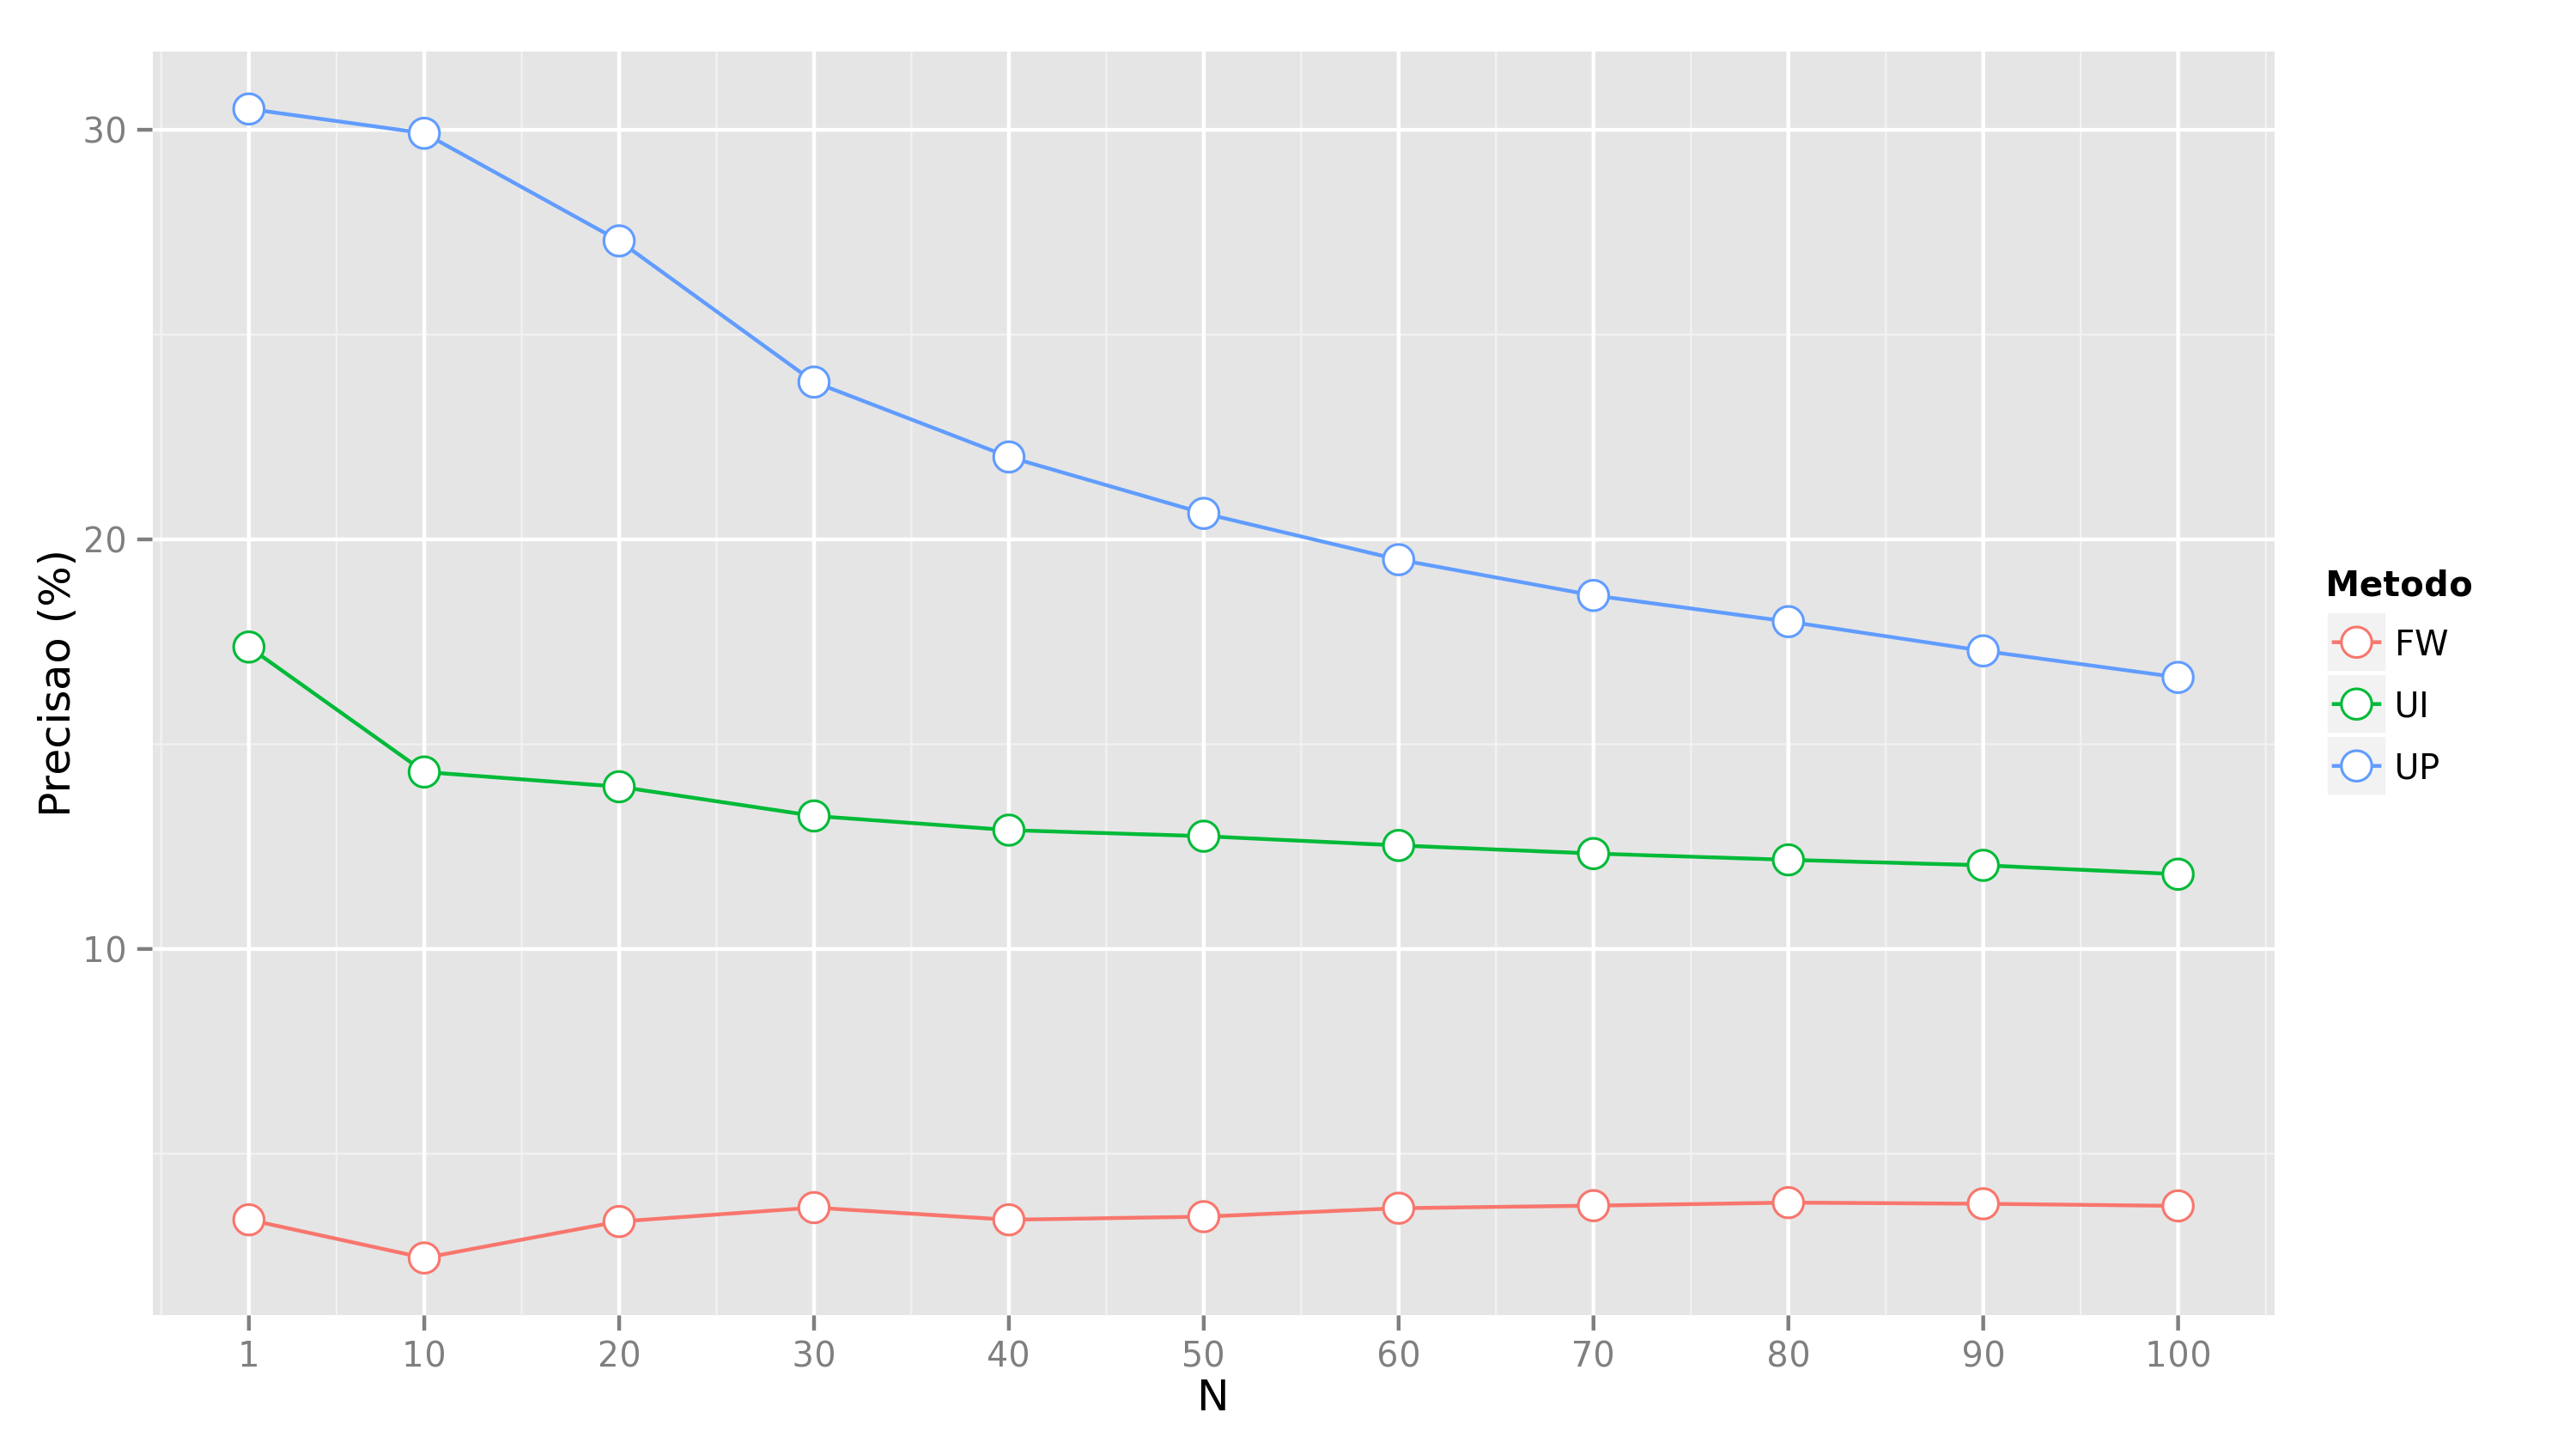
\includegraphics[width=1\textwidth]{img/precision_N}
    \end{center}
    \label{fig:precision_N}
    \caption{Precisão em função do tamanho da lista de recomendações $N$}
\end{figure}


\begin{figure}[htp]
    \begin{center}
    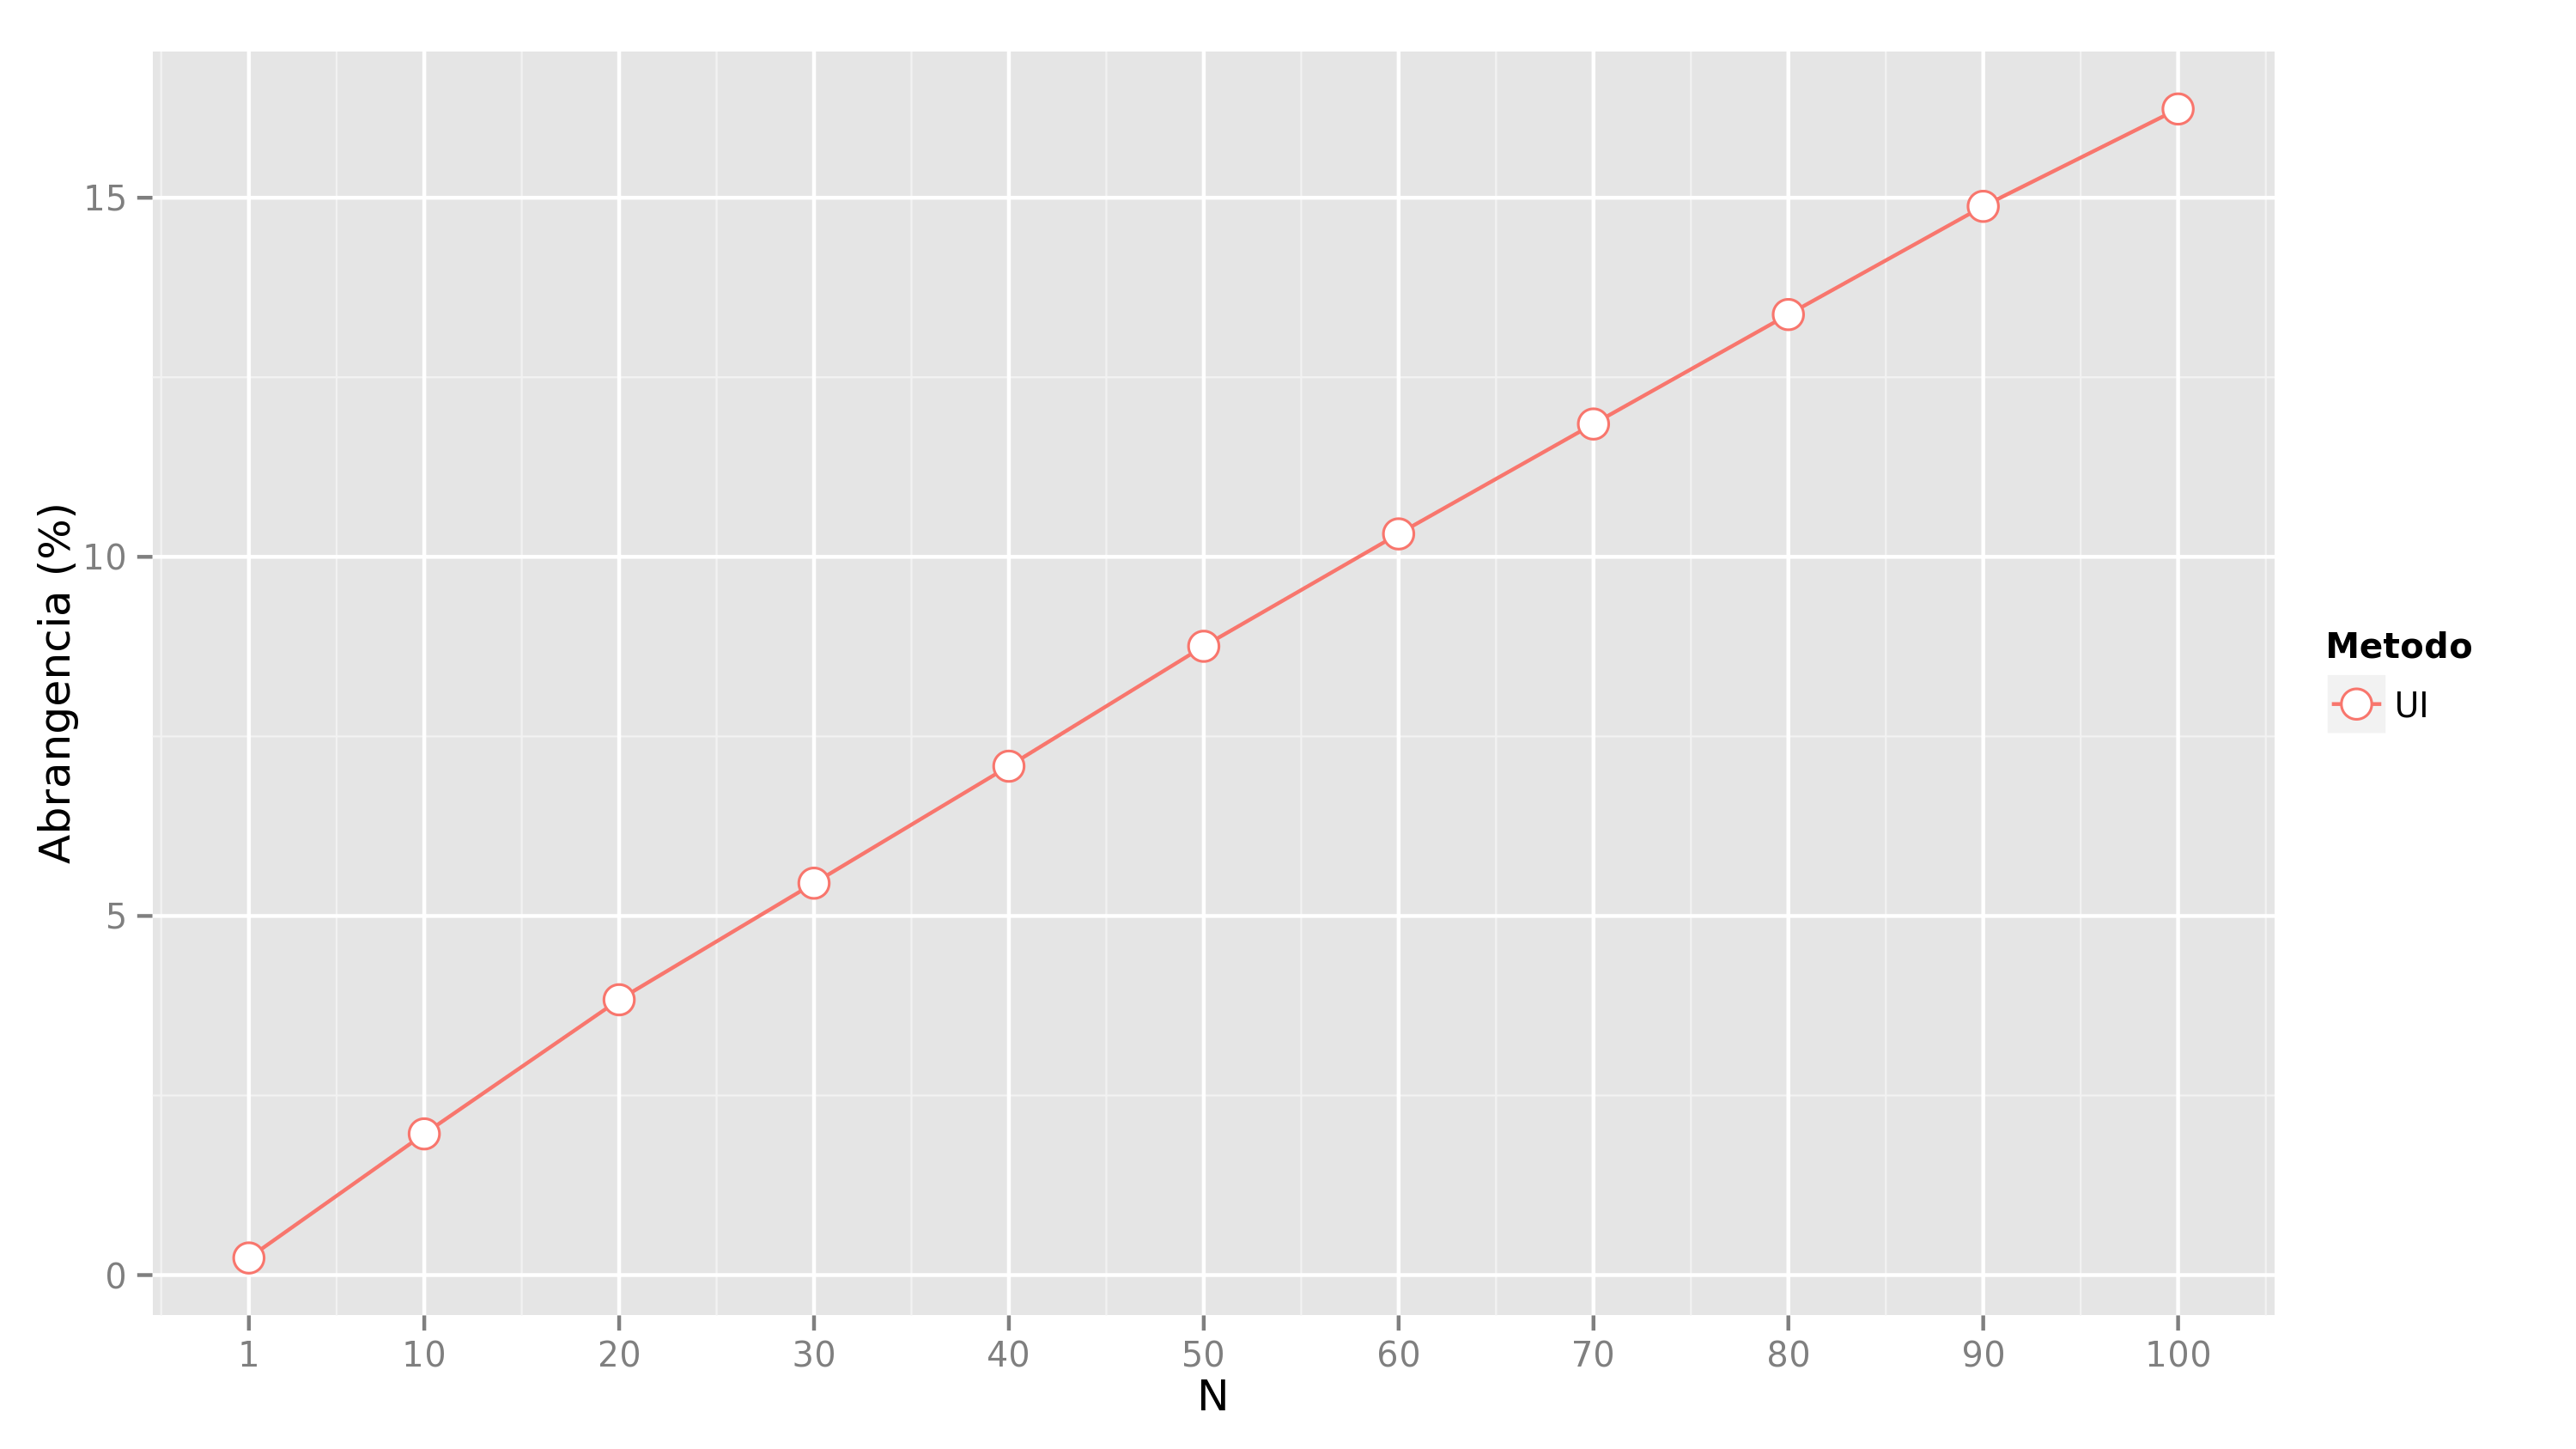
\includegraphics[width=1\textwidth]{img/recall_N}
    \end{center}
    \label{fig:recall_N}
    \caption{Abrangência em função do tamanho da lista de recomendações $N$}
\end{figure}

\begin{figure}[htp]
    \begin{center}
    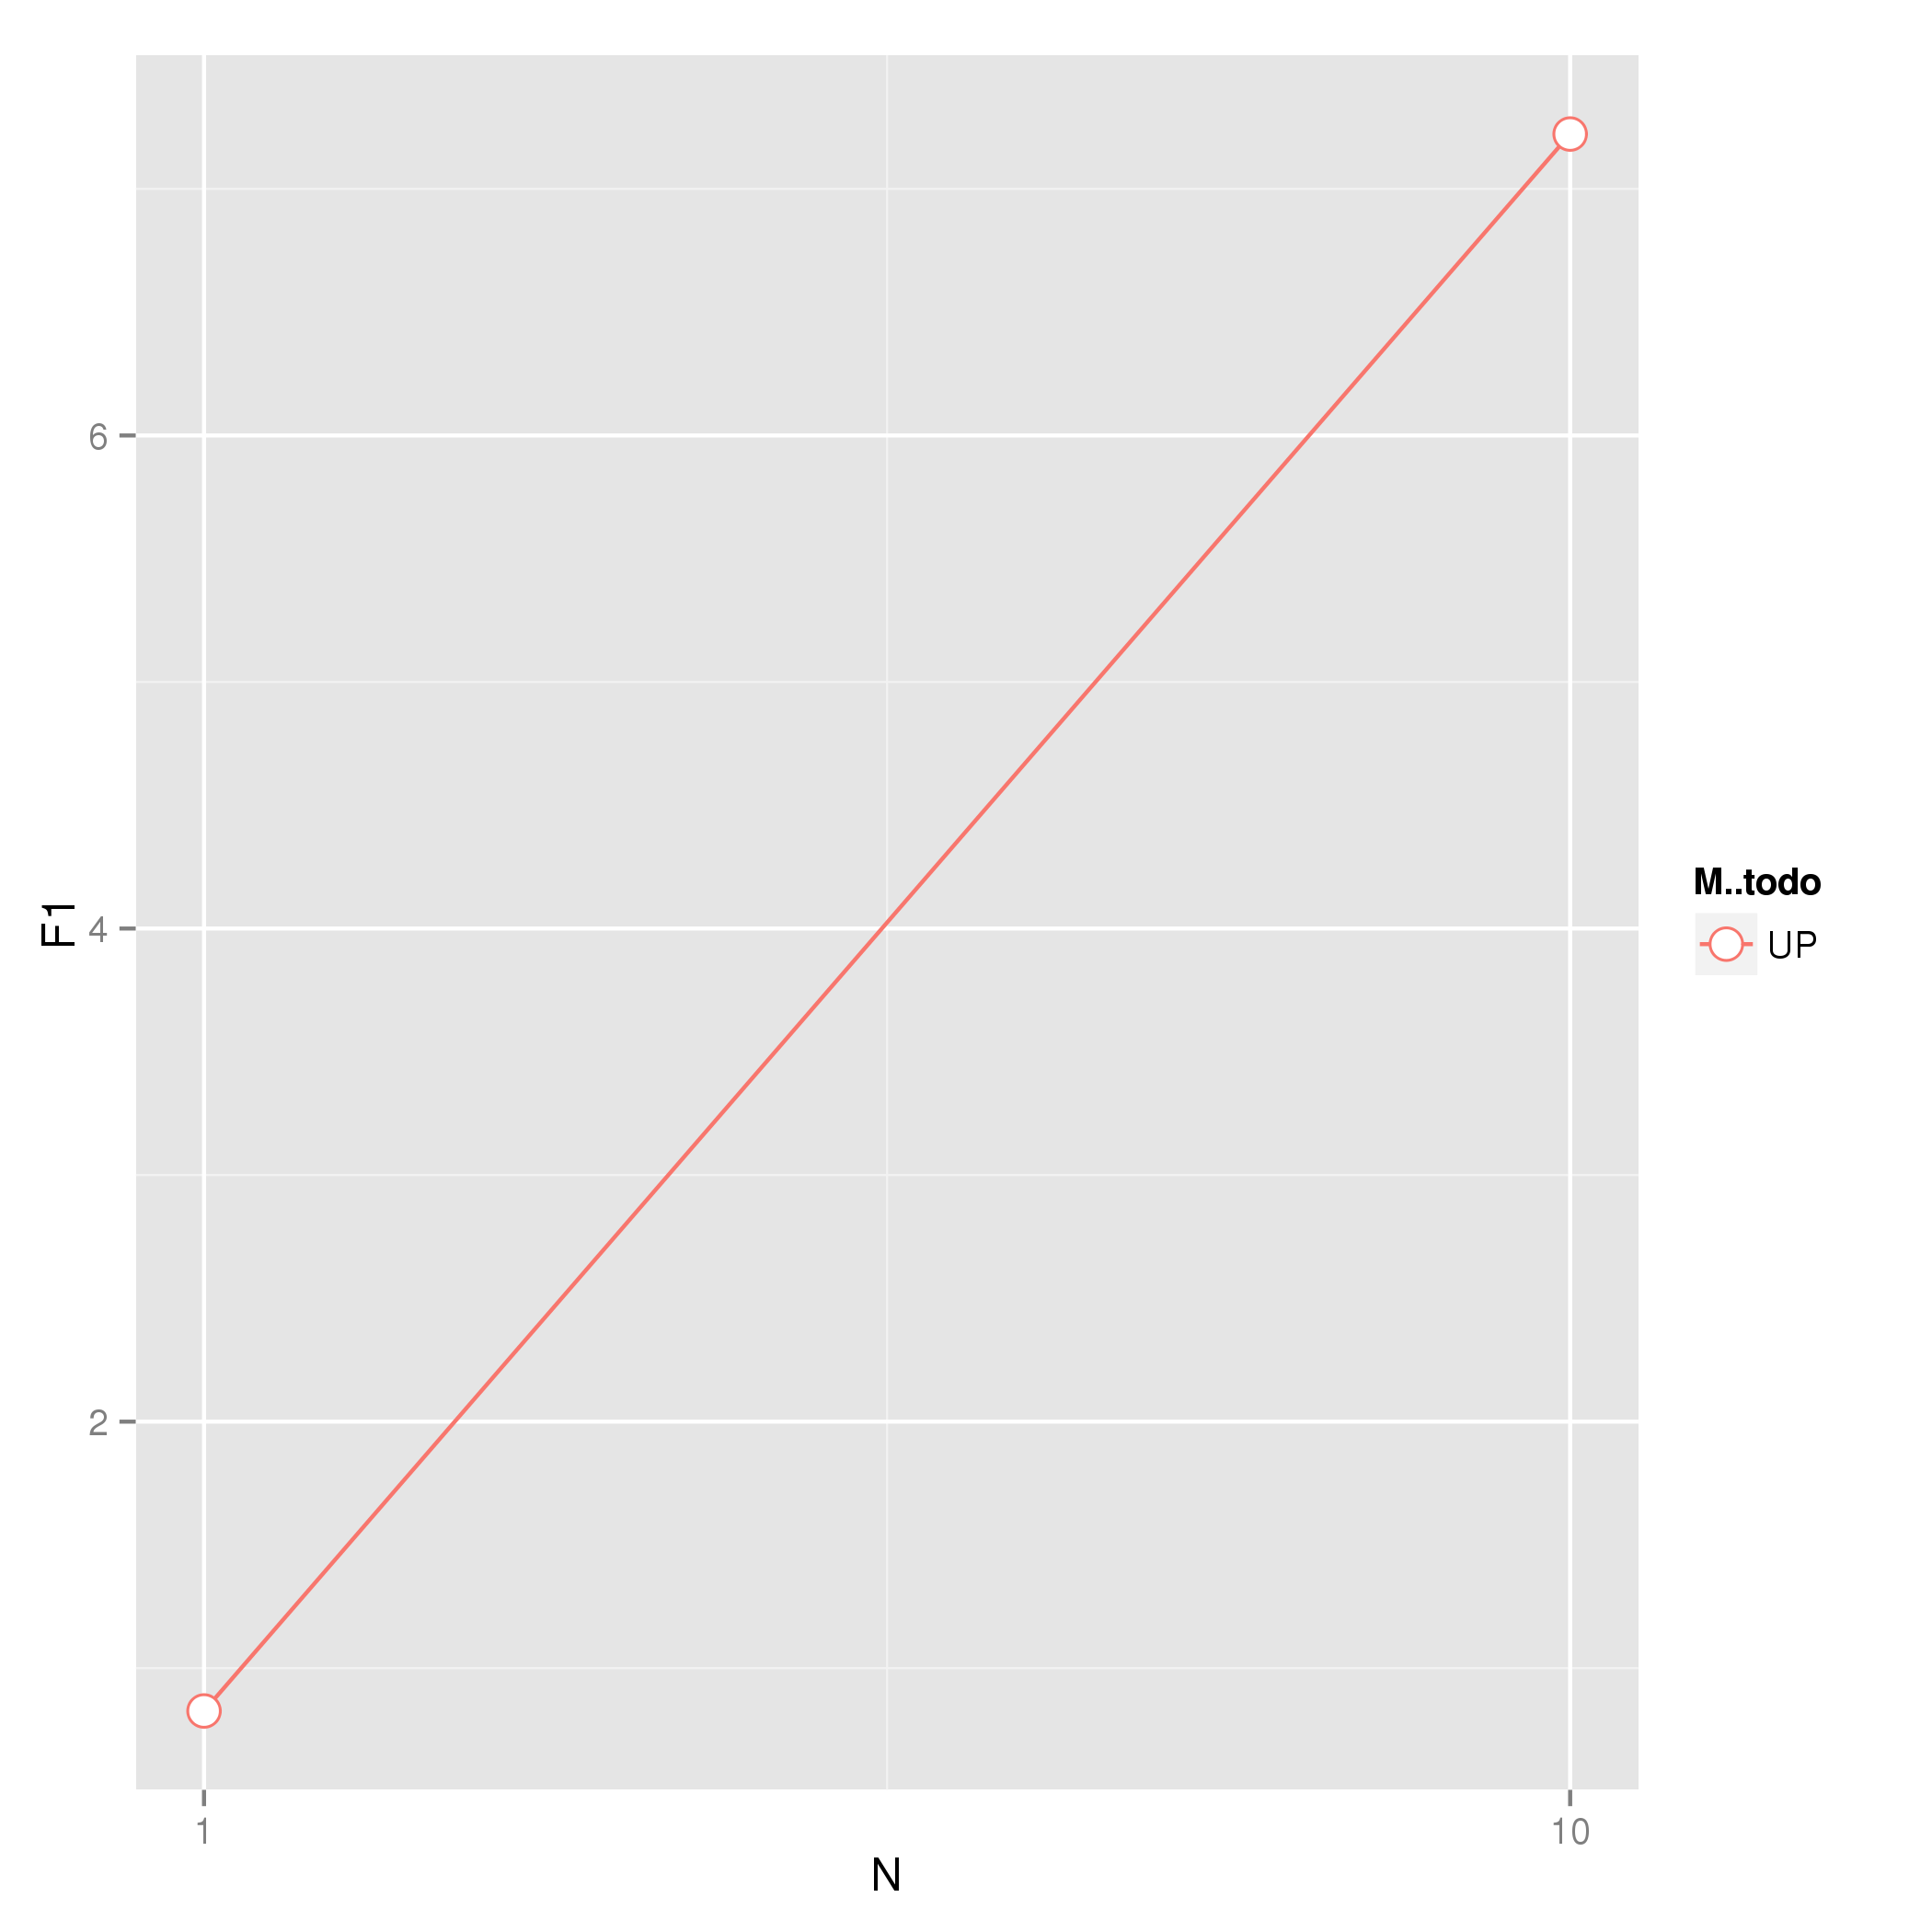
\includegraphics[width=1\textwidth]{img/F1_N}
    \end{center}
    \label{fig:F1_N}
    \caption{Medida $F_1$ em função do tamanho da lista de recomendações $N$}
\end{figure}

\begin{figure}[htp]
    \begin{center}
    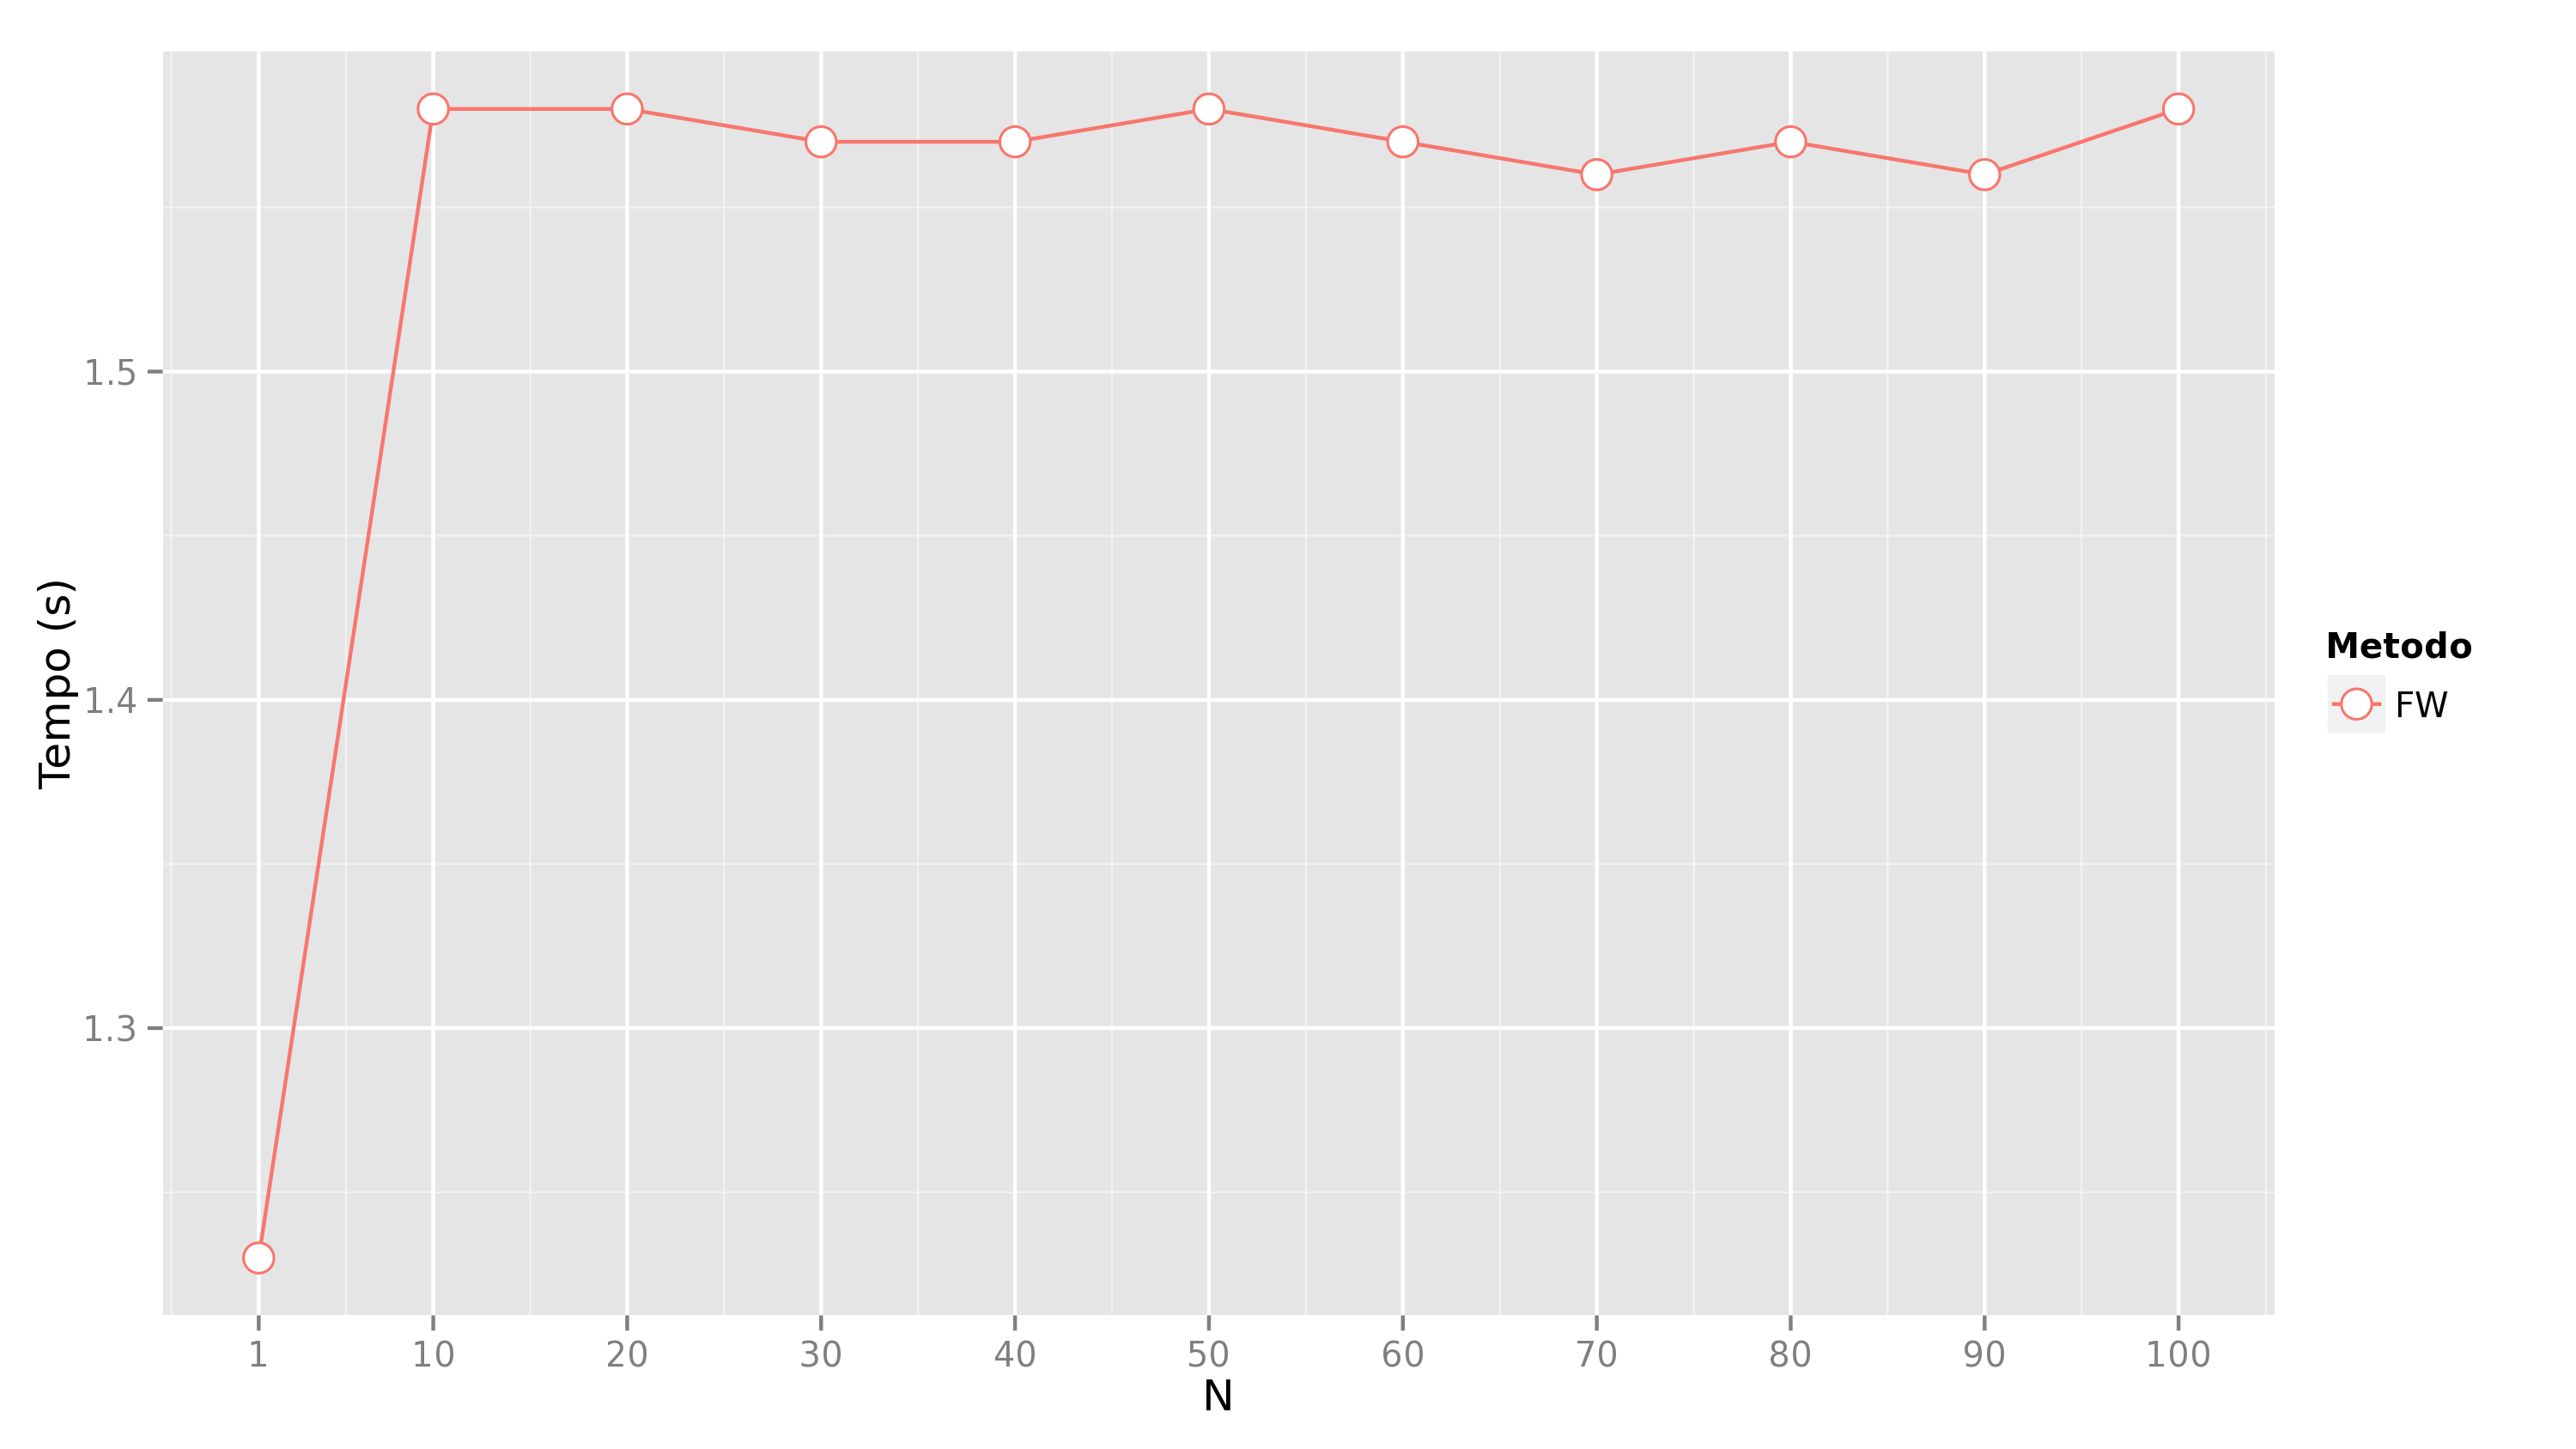
\includegraphics[width=1\textwidth]{img/time_N}
    \end{center}
    \label{fig:time_N}
    \caption{Tempo de execução em função do tamanho da lista de recomendações $N$}
\end{figure}

Contrariamente ao esperado, a qualidade de recomendação do algoritmo UI é sensivelmente inferior à do algoritmo UP. Isso se deve ao fato de a correlação usuário-item daquele método colocar ênfase no valor do atributo $a_{if}$, mesmo que esses atributos não sejam diretamente proporcionais à preferência do usuário. Esse cálculo é incoerente, por exemplo, para atributos $f=\mathrm{data}$: mesmo que o usuário tenha um elevado interesse $w_{uf}$ por filmes antigos, o valor de $a_{if}$ não leva em conta se sua preferência é por filmes da década de 1970 ou 1990. Nesse caso, o algoritmo indicaria incorretamente que filmes mais recentes são mais adequados para aquele usuário, porque possuem maior $a_{if}$.

A fim de corrigir essa falha no algoritmo UI, seria necessário, por exemplo, aplicar nos atributos $a_{if}$ uma função $g_f$ que crescesse no mesmo sentido do interesse do usuário por aquela \textit{feature}. Dessa forma, o cálculo $\sum_f w_{uf}~g_f\left(a_{if}\right)$ significaria de fato a similaridade entre o usuário $u$ e o item $i$ medida através de seu interesse $g\left(a_{if}\right)$ pelas \textit{features} $f$.

Apesar de alta qualidade das recomendações do método UP, este possui também a maior complexidade computacional. Seu tempo de execução é 2 vezes maior que o do método FW e 4 vezes maior que o do método UI. Todavia, nenhum desses tempos de execução é crítico, tendo em vista que o sistema não seria colocado diretamente à disposição dos clientes, mas que as recomendações seriam enviadas via email, por exemplo. 

Apenas o método UI atende ao requisito de \textit{throughput} mínimo de 28 recomendações para cada usuário por segundo. Dado que a base de testes possui $25\%$ do total de usuários, correspondente a 236 clientes para o banco 100k, o tempo de execução máximo dos métodos deveria ser de $0.15$ min. A fim de melhorar a velocidade das recomendações, a solução mais eficiente é a mudança da linguagem de programação. O uso de linguagens C, C++ ou Python pode melhorar o desempenho computacional em até 500 vezes \cite{benchmarkingR}. 

\section{Percentual da base de aprendizado $T$} % (fold)
\label{sec:percentual_da_base_de_aprendizado_}

A medida que o percentual da base de aprendizados aumenta, a precisão de todos os métodos cresce ligeiramente. Isso é consequência do caráter colaborativo dos algoritmos, já que a qualidade da recomendação depende da quantidade total de dados. Entretanto, pode-se observar que a abrangência e a medida $F_1$ são praticamente constantes para valores crescentes de $T$ de modo que esse parâmetro não tem grande relevância para o sucesso do sistema de recomendação.

O parâmetro $T$ não exerce nenhuma influência sobre o tempo de execução dos métodos UP e UI, mas apenas sobre o método FW. Isso ocorre porque a etapa de maior custo computacional (Equação \ref{eq:determinacao-wf}) é linearmente dependente da quantidade de usuários $\left|\mathcal{U}\right|$. Quanto menos usuários-teste, mais veloz é o algoritmo.

\begin{figure}[htp]
    \begin{center}
    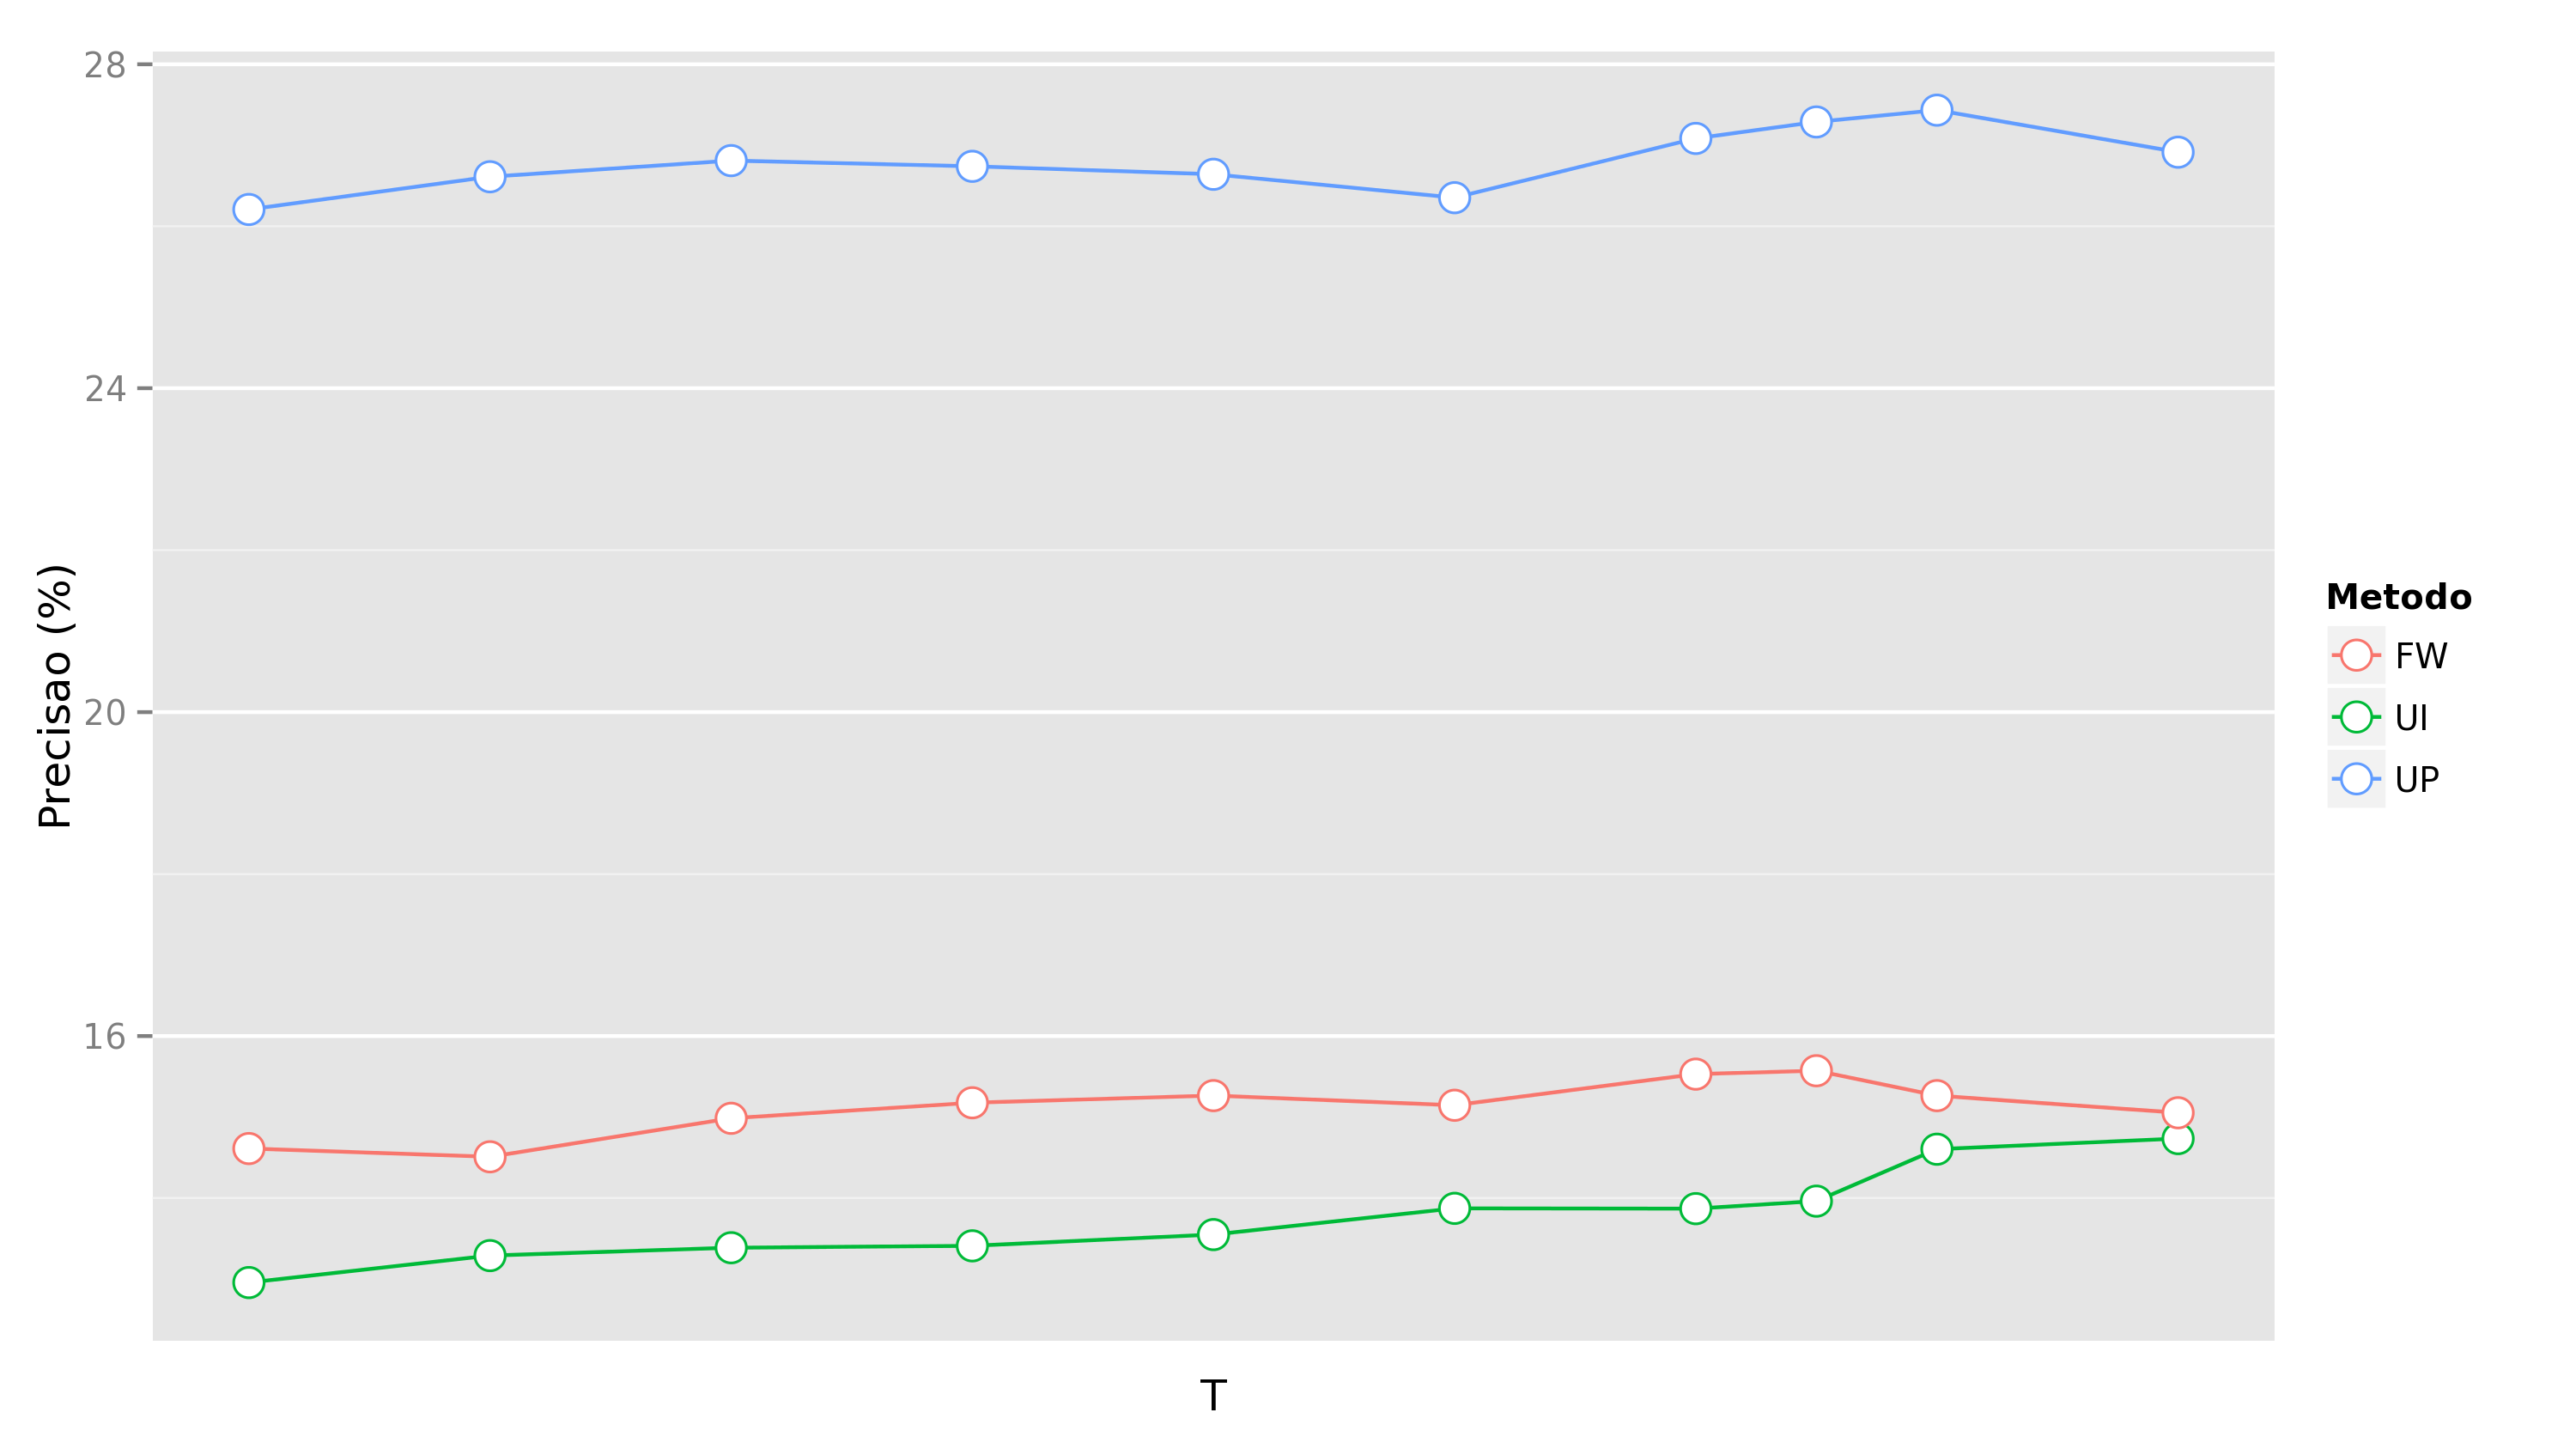
\includegraphics[width=1\textwidth]{img/precision_T}
    \end{center}
    \label{fig:precision_T}
    \caption{Precisão em função do percentual da base de aprendizado $T$}
\end{figure}


\begin{figure}[htp]
    \begin{center}
    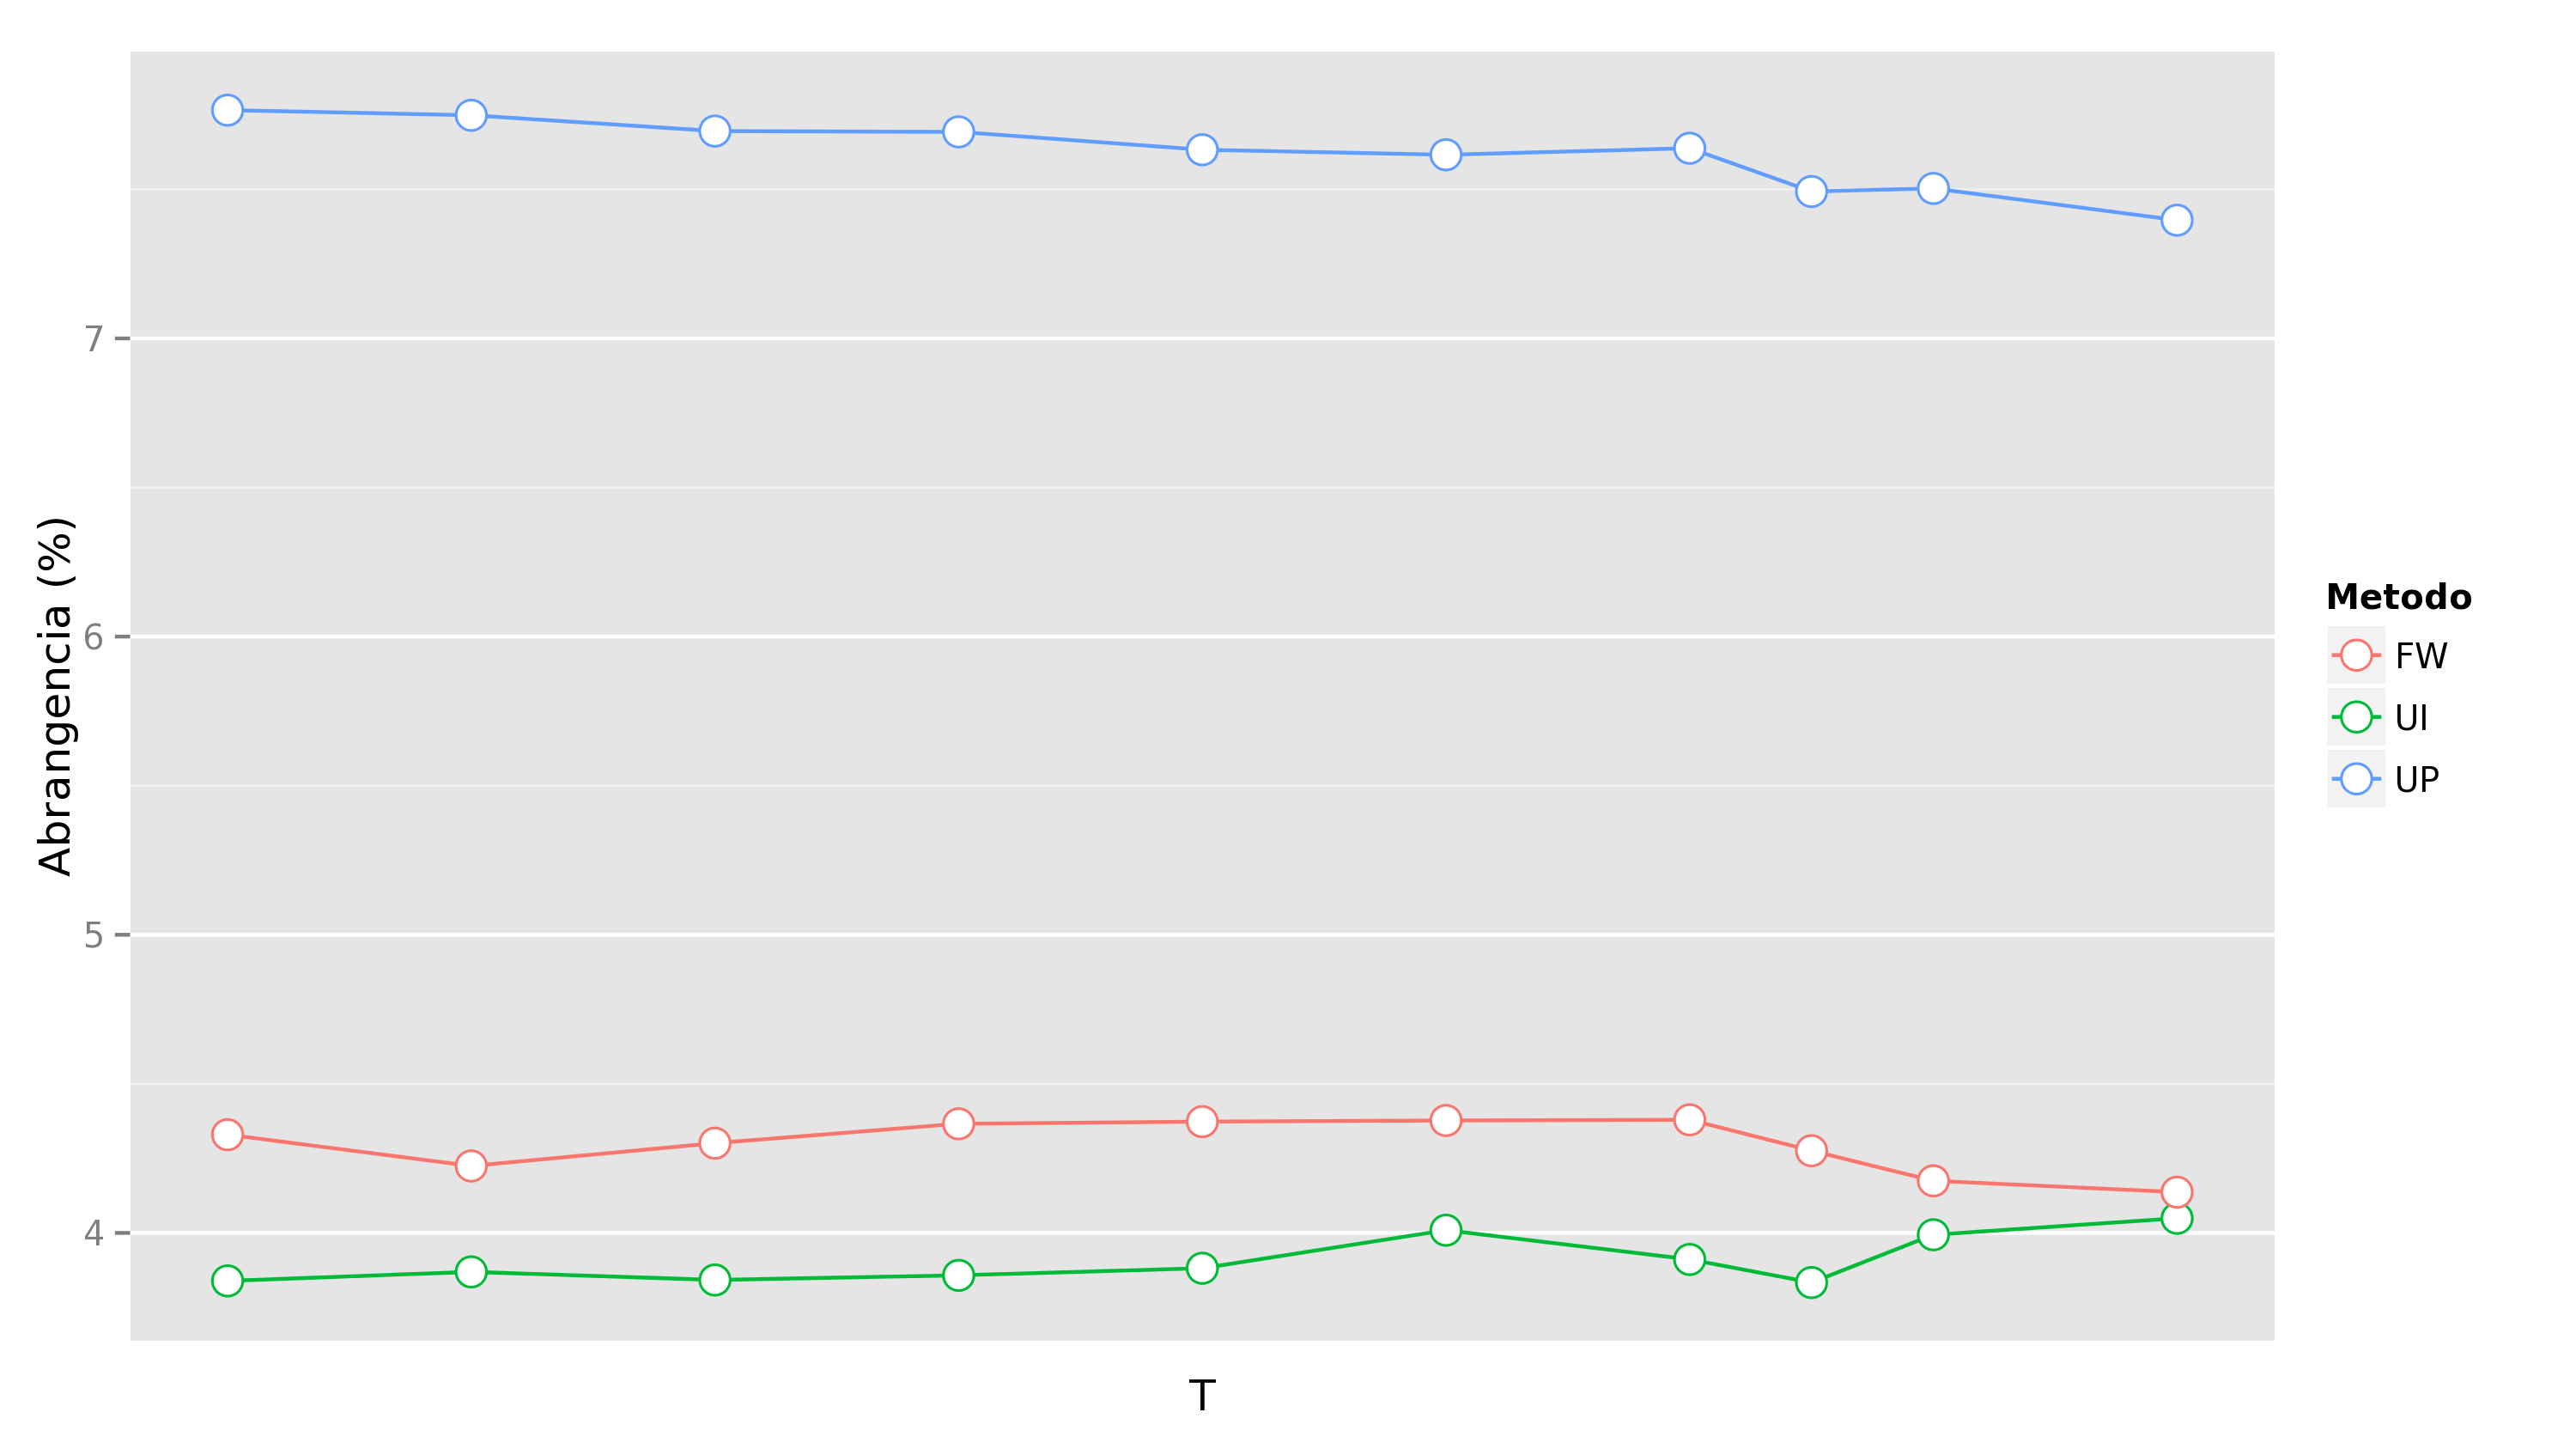
\includegraphics[width=1\textwidth]{img/recall_T}
    \end{center}
    \label{fig:recall_T}
    \caption{Abrangência em função do percentual da base de aprendizado $T$}
\end{figure}

\begin{figure}[htp]
    \begin{center}
    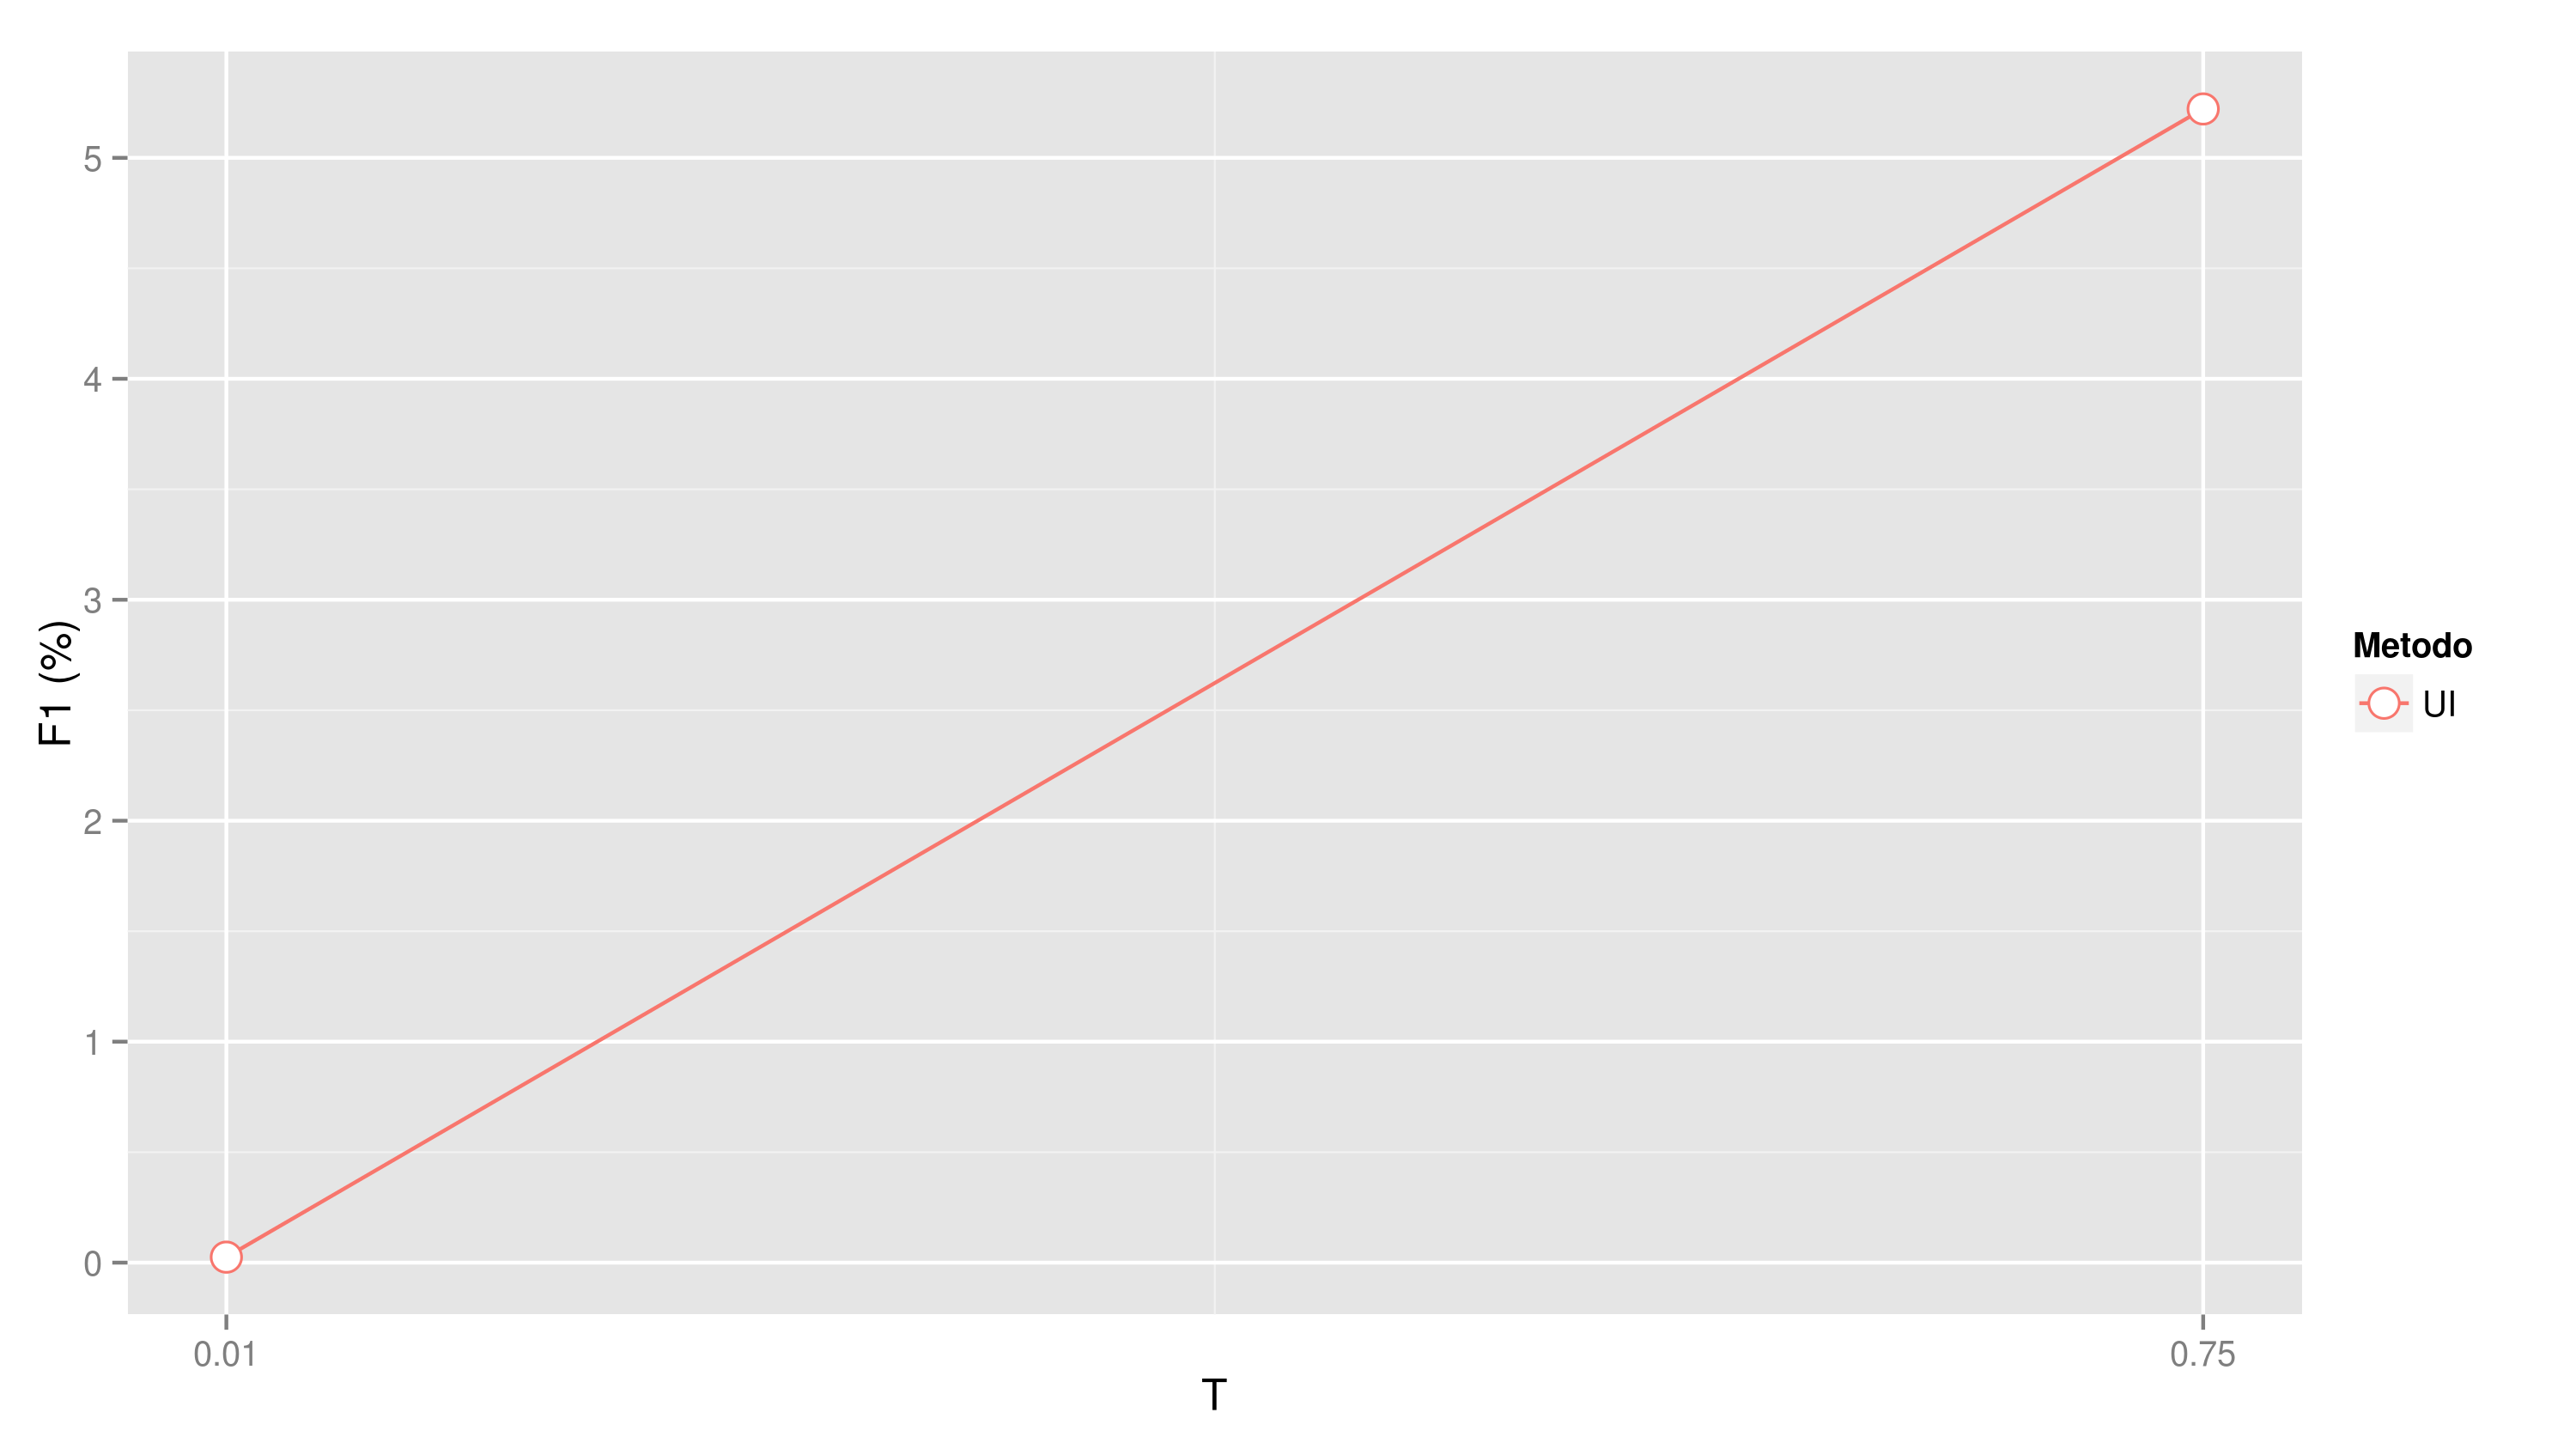
\includegraphics[width=1\textwidth]{img/F1_T}
    \end{center}
    \label{fig:F1_T}
    \caption{Medida $F_1$ em função do percentual da base de aprendizado $T$}
\end{figure}

\begin{figure}[htp]
    \begin{center}
    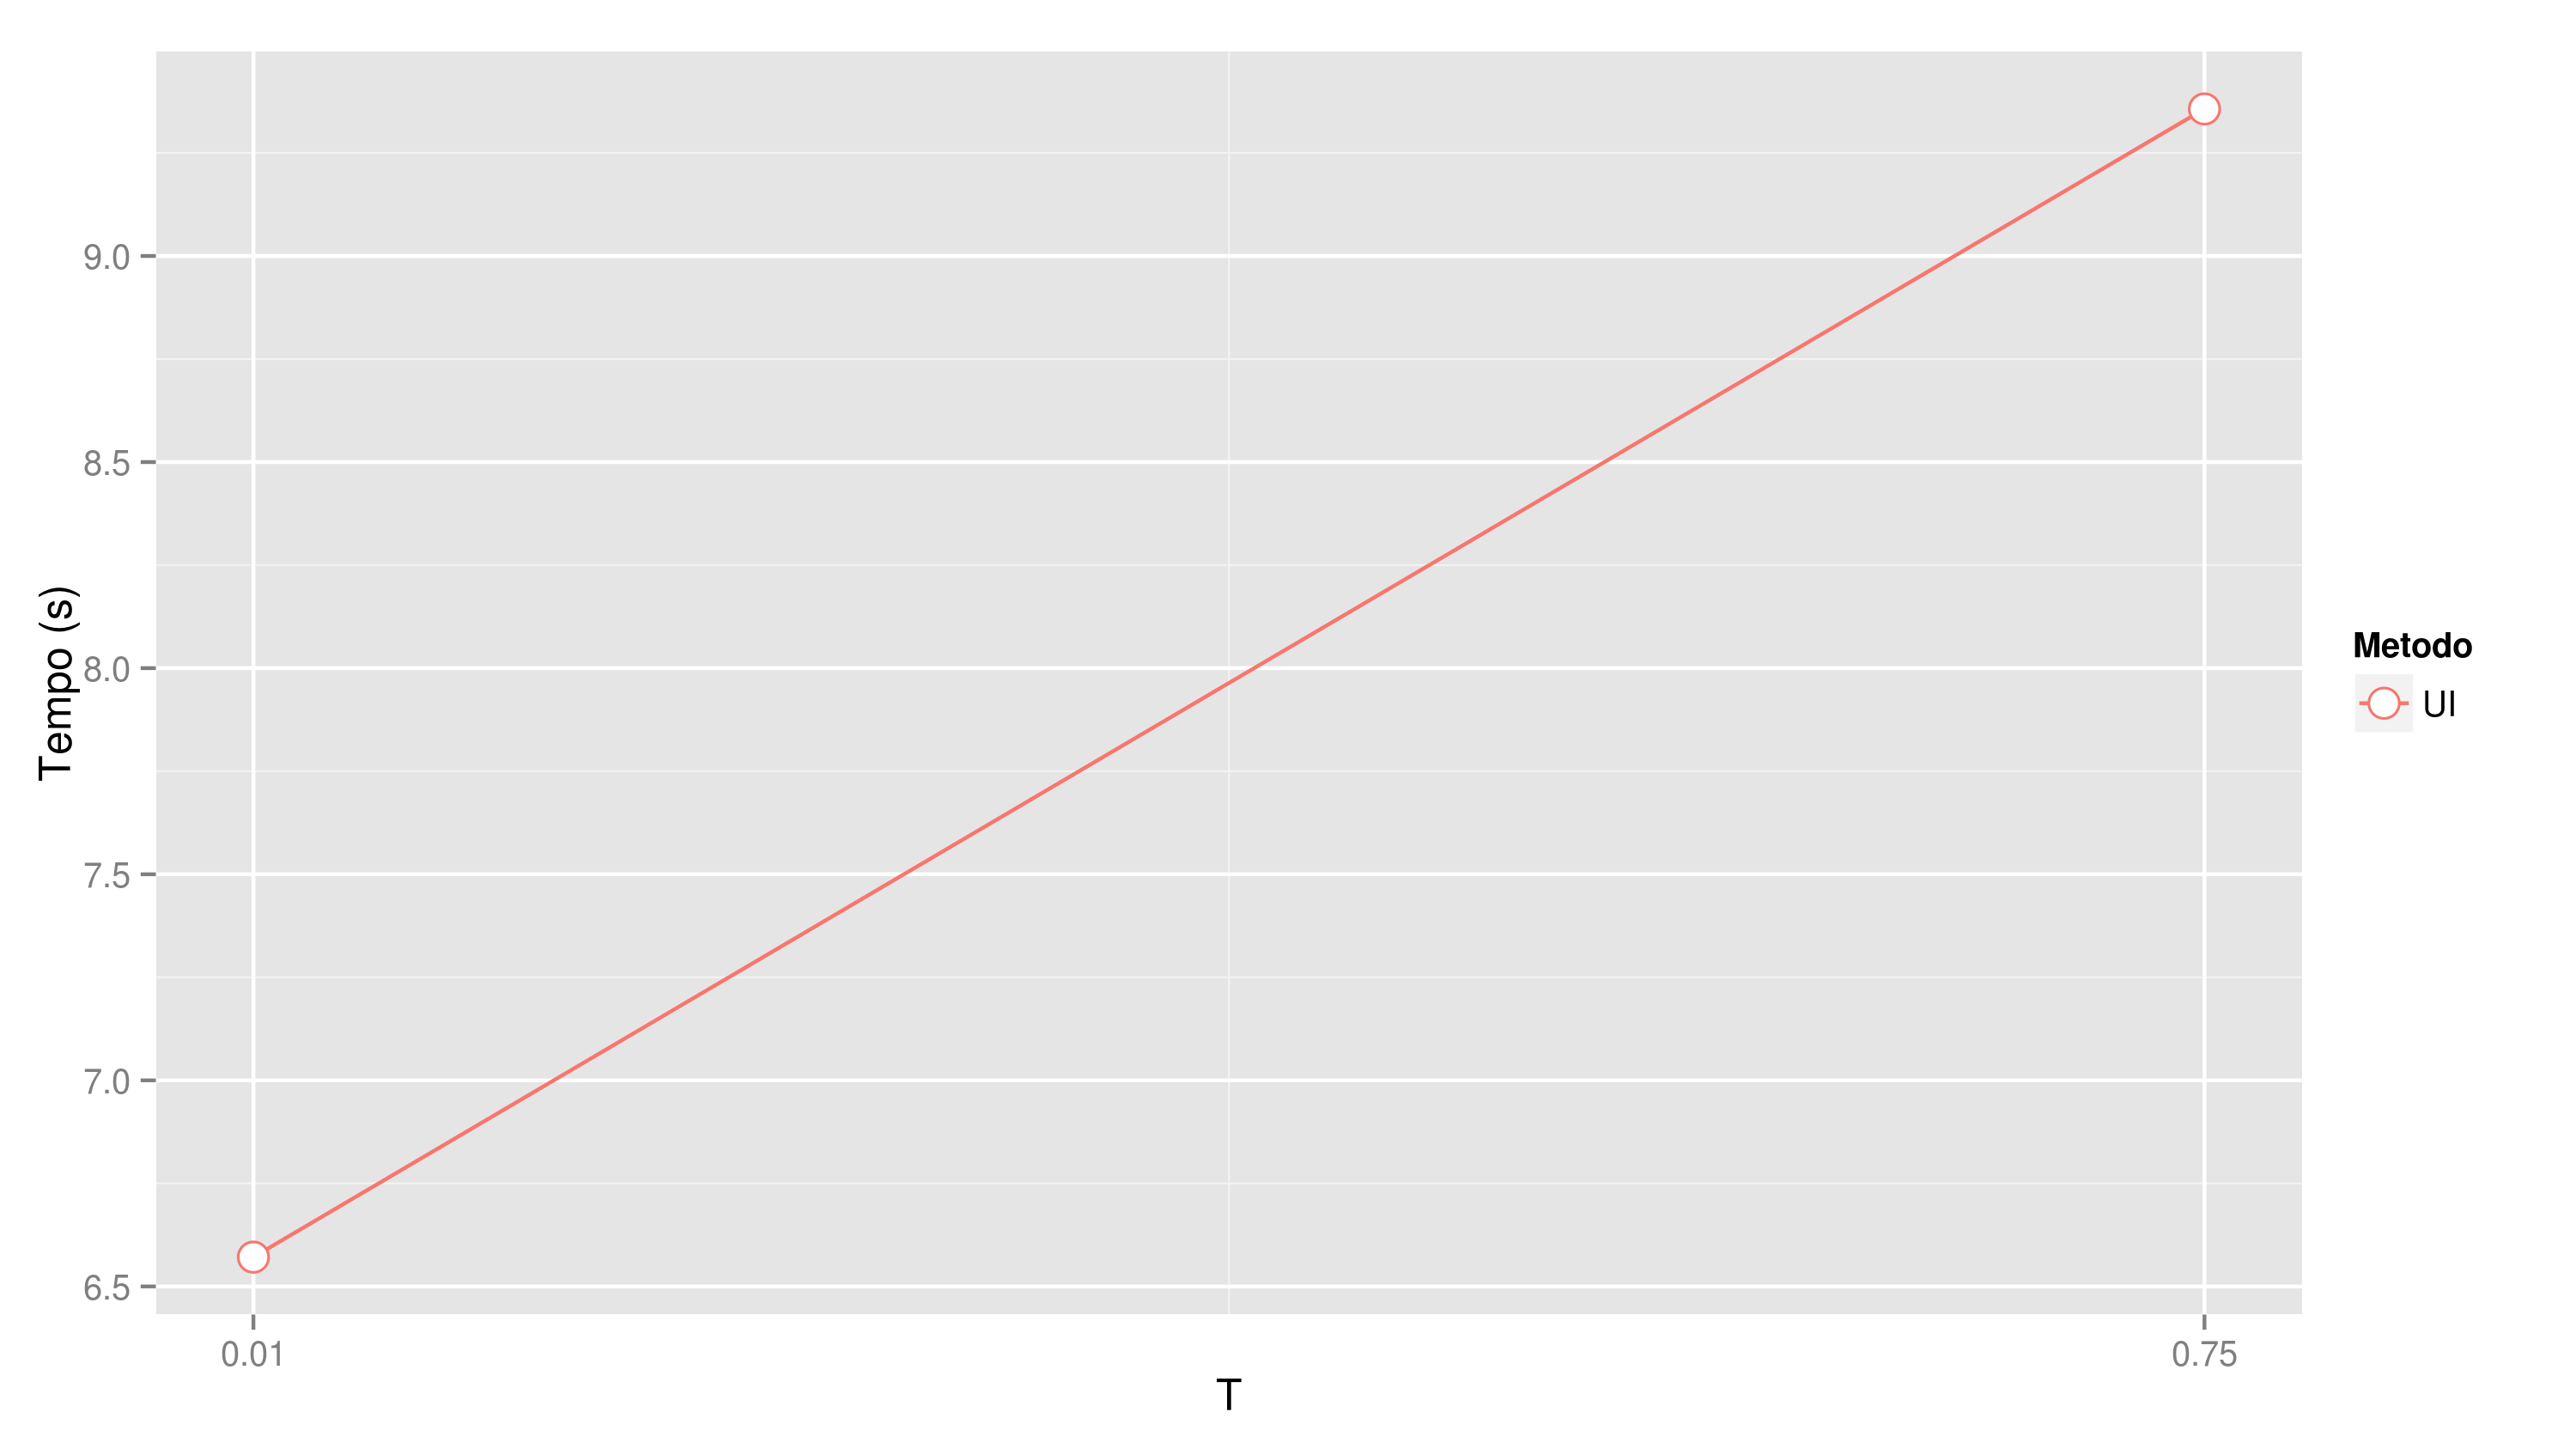
\includegraphics[width=1\textwidth]{img/time_T}
    \end{center}
    \label{fig:time_T}
    \caption{Tempo de execução em função do percentual da base de aprendizado $T$}
\end{figure}


\section{Percentual de avaliações ``escondidas'' dos usuários-teste na validação cruzada $H$} % (fold)
\label{sec:percentual_de_avalia_es_dos_usu_rios_teste_na_valida_o_cruzada}

Quanto maior o número de avaliações ``escondidas'', mais fácil é acertar os itens dos usuários-teste, pois a lista de recomendação é pequena em relação ao total de itens positivamente avaliados pelo usuário. Por esse motivo, a precisão cresce com $H$ para todos os métodos. 

Para o algoritmo FW, a precisão atinge seu máximo em $H=75\%$ e depois decresce ligeiramente. Isso ocorre porque o cálculo dos pesos $w_f$ depende da quantidade de avaliações $r_{ui}$. Existe, pois, um compromisso (\textit{tradeoff}) entre facilidade de se acertar itens avaliados quando há muitas avaliações escondidas e a dificuldade de se estimar $w_f$ quando não há muitos dados de avaliações.  

Ao passo que a precisão dos métodos aumenta com $H$, a abrangência diminui. Visto que a quantidade de itens da lista \textit{top-}$N$ é fixa, quanto maior o número de itens ``escondidos'', mais difícil é de se retornar todos os itens relevantes.

O resultado de uma precisão crescente em função de $H$ e uma acurácia decrescente é que a medida $F_1$ possui um ponto de máximo. Para todos os métodos, o valor máximo é tal que $H=50\%$.

Quanto ao tempo de execução, a influência é a mesma do parâmetro $T$: 
para o método FW, a etapa de maior custo computacional (Equação \ref{eq:determinacao-wf}) é linearmente dependente da quantidade de itens $\left|\mathcal{I}\right|$. Quanto menos avaliações de itens dos usuários-teste, mais veloz é o algoritmo.


\begin{figure}[htp]
    \begin{center}
    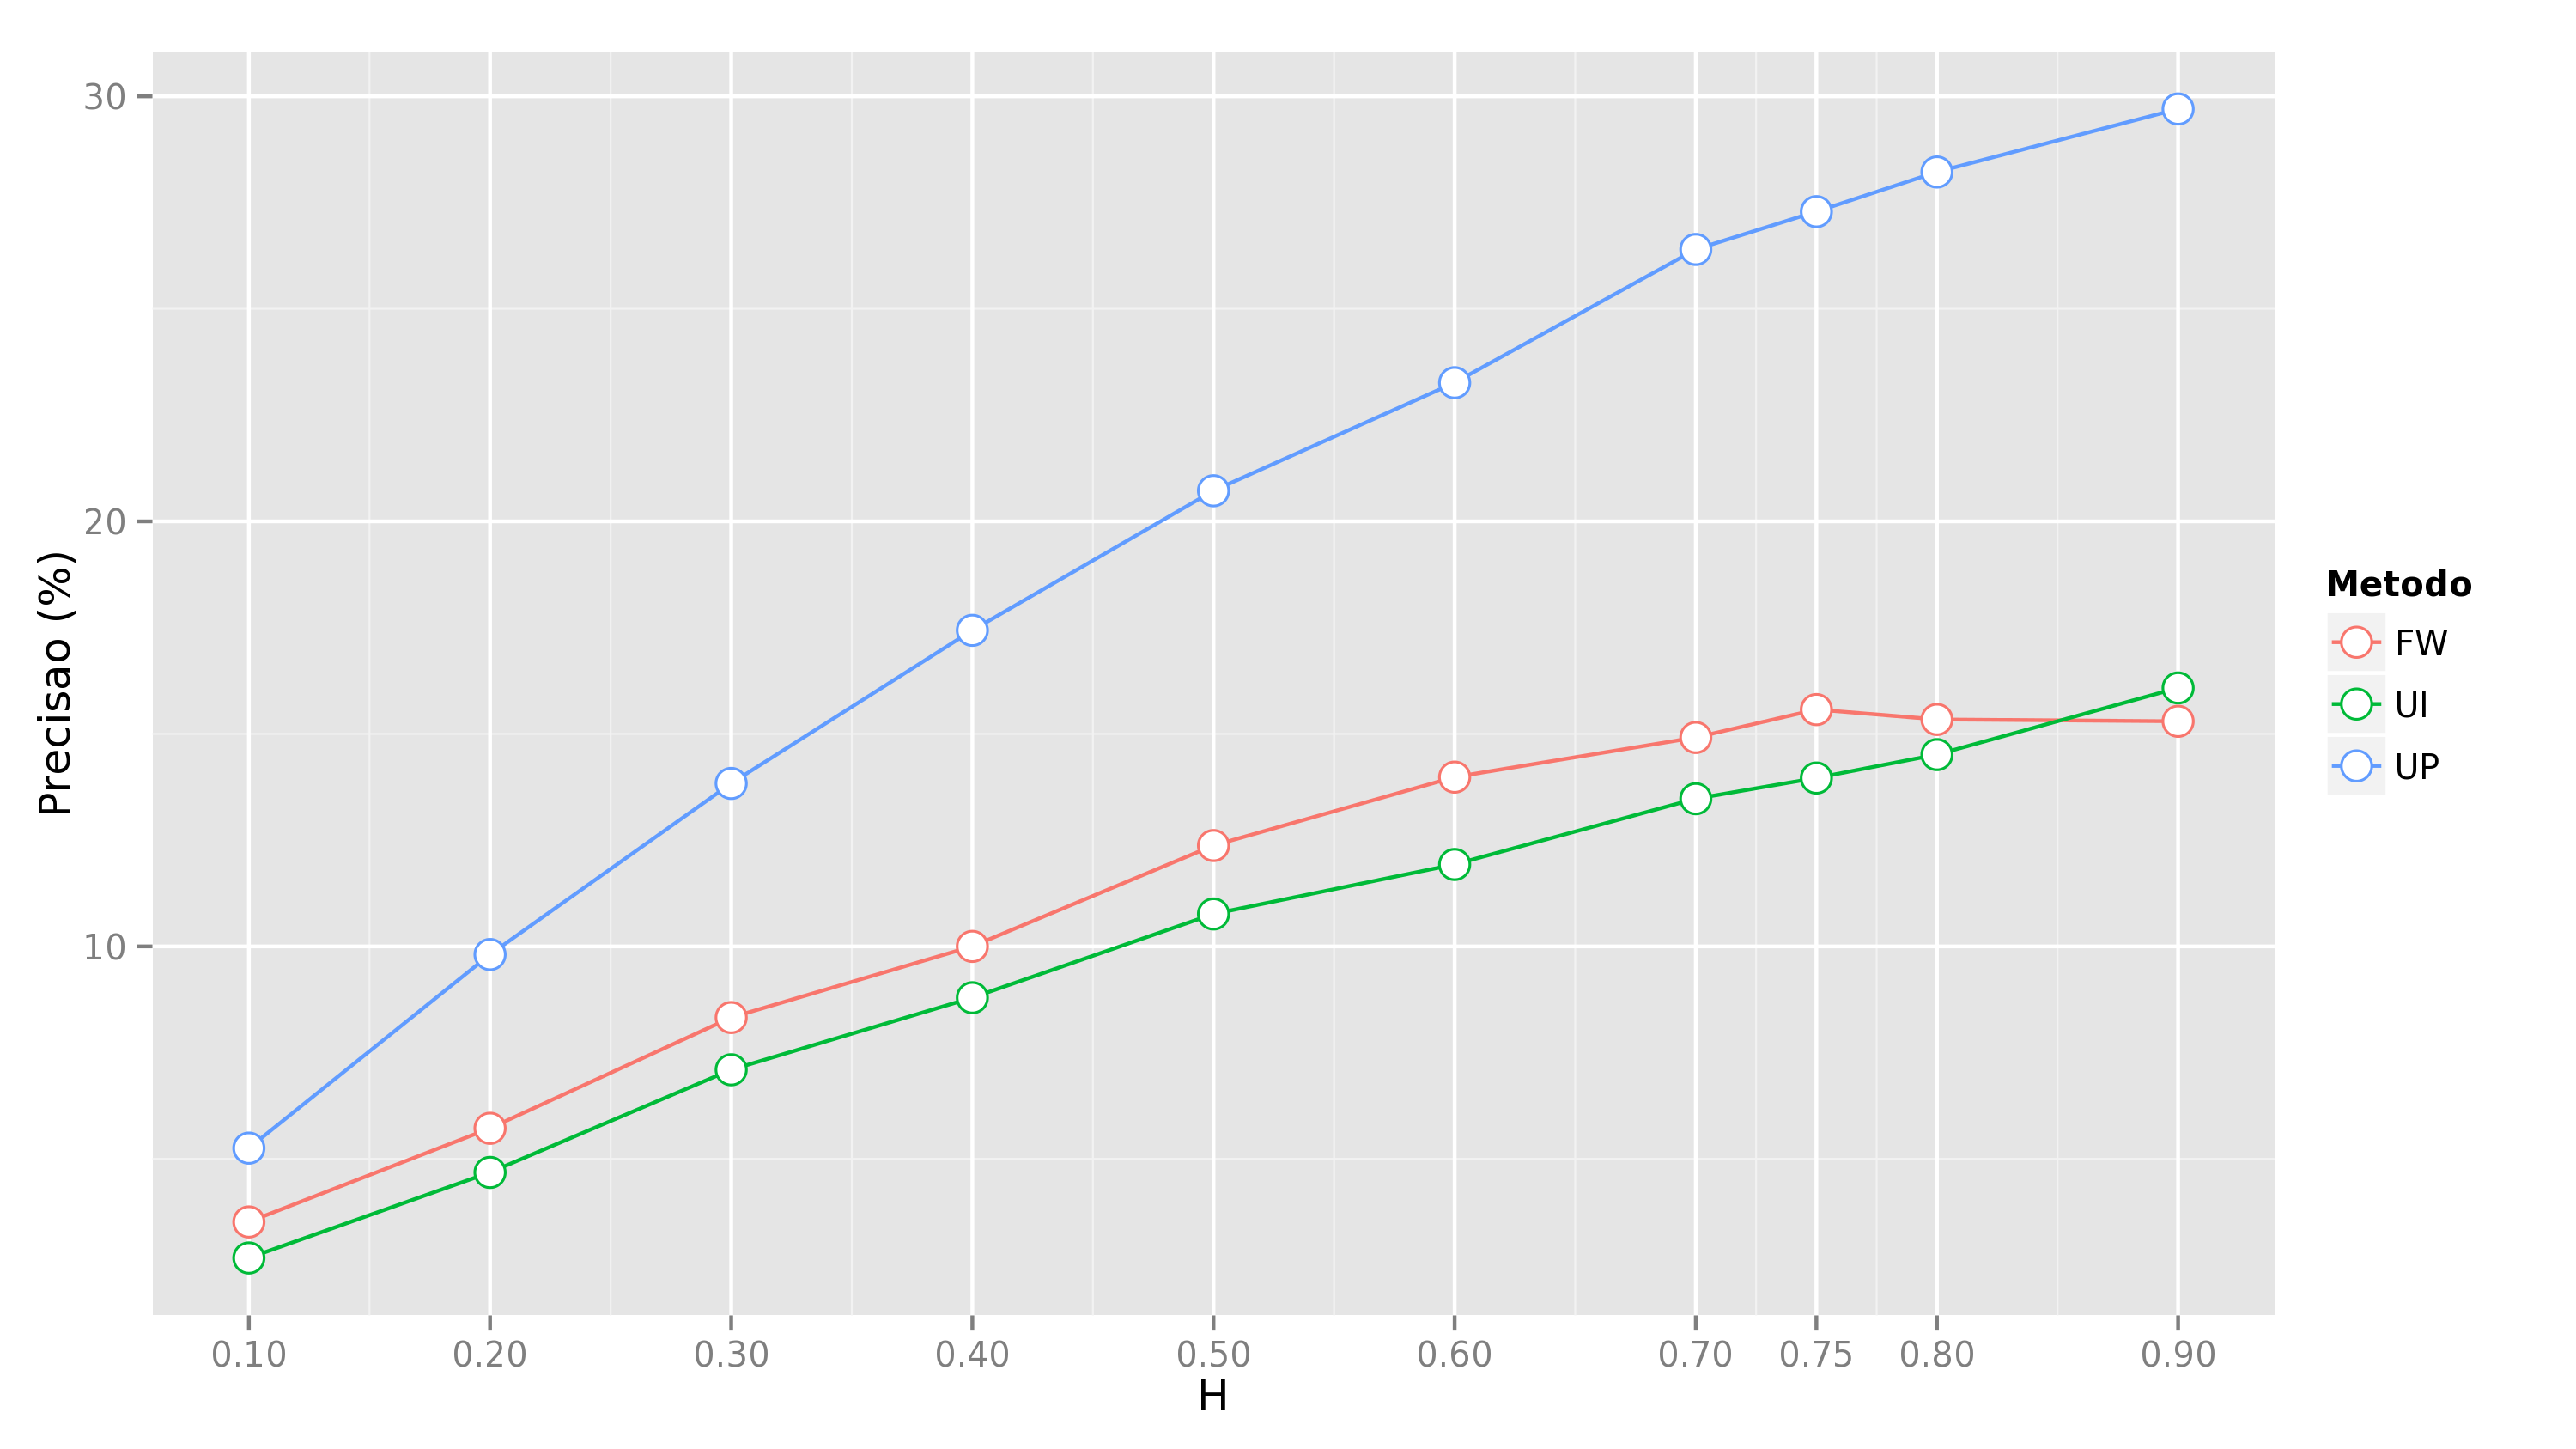
\includegraphics[width=1\textwidth]{img/precision_H}
    \end{center}
    \label{fig:precision_H}
    \caption{Precisão em função do percentual de avaliações ``escondidas'' $H$}
\end{figure}


\begin{figure}[htp]
    \begin{center}
    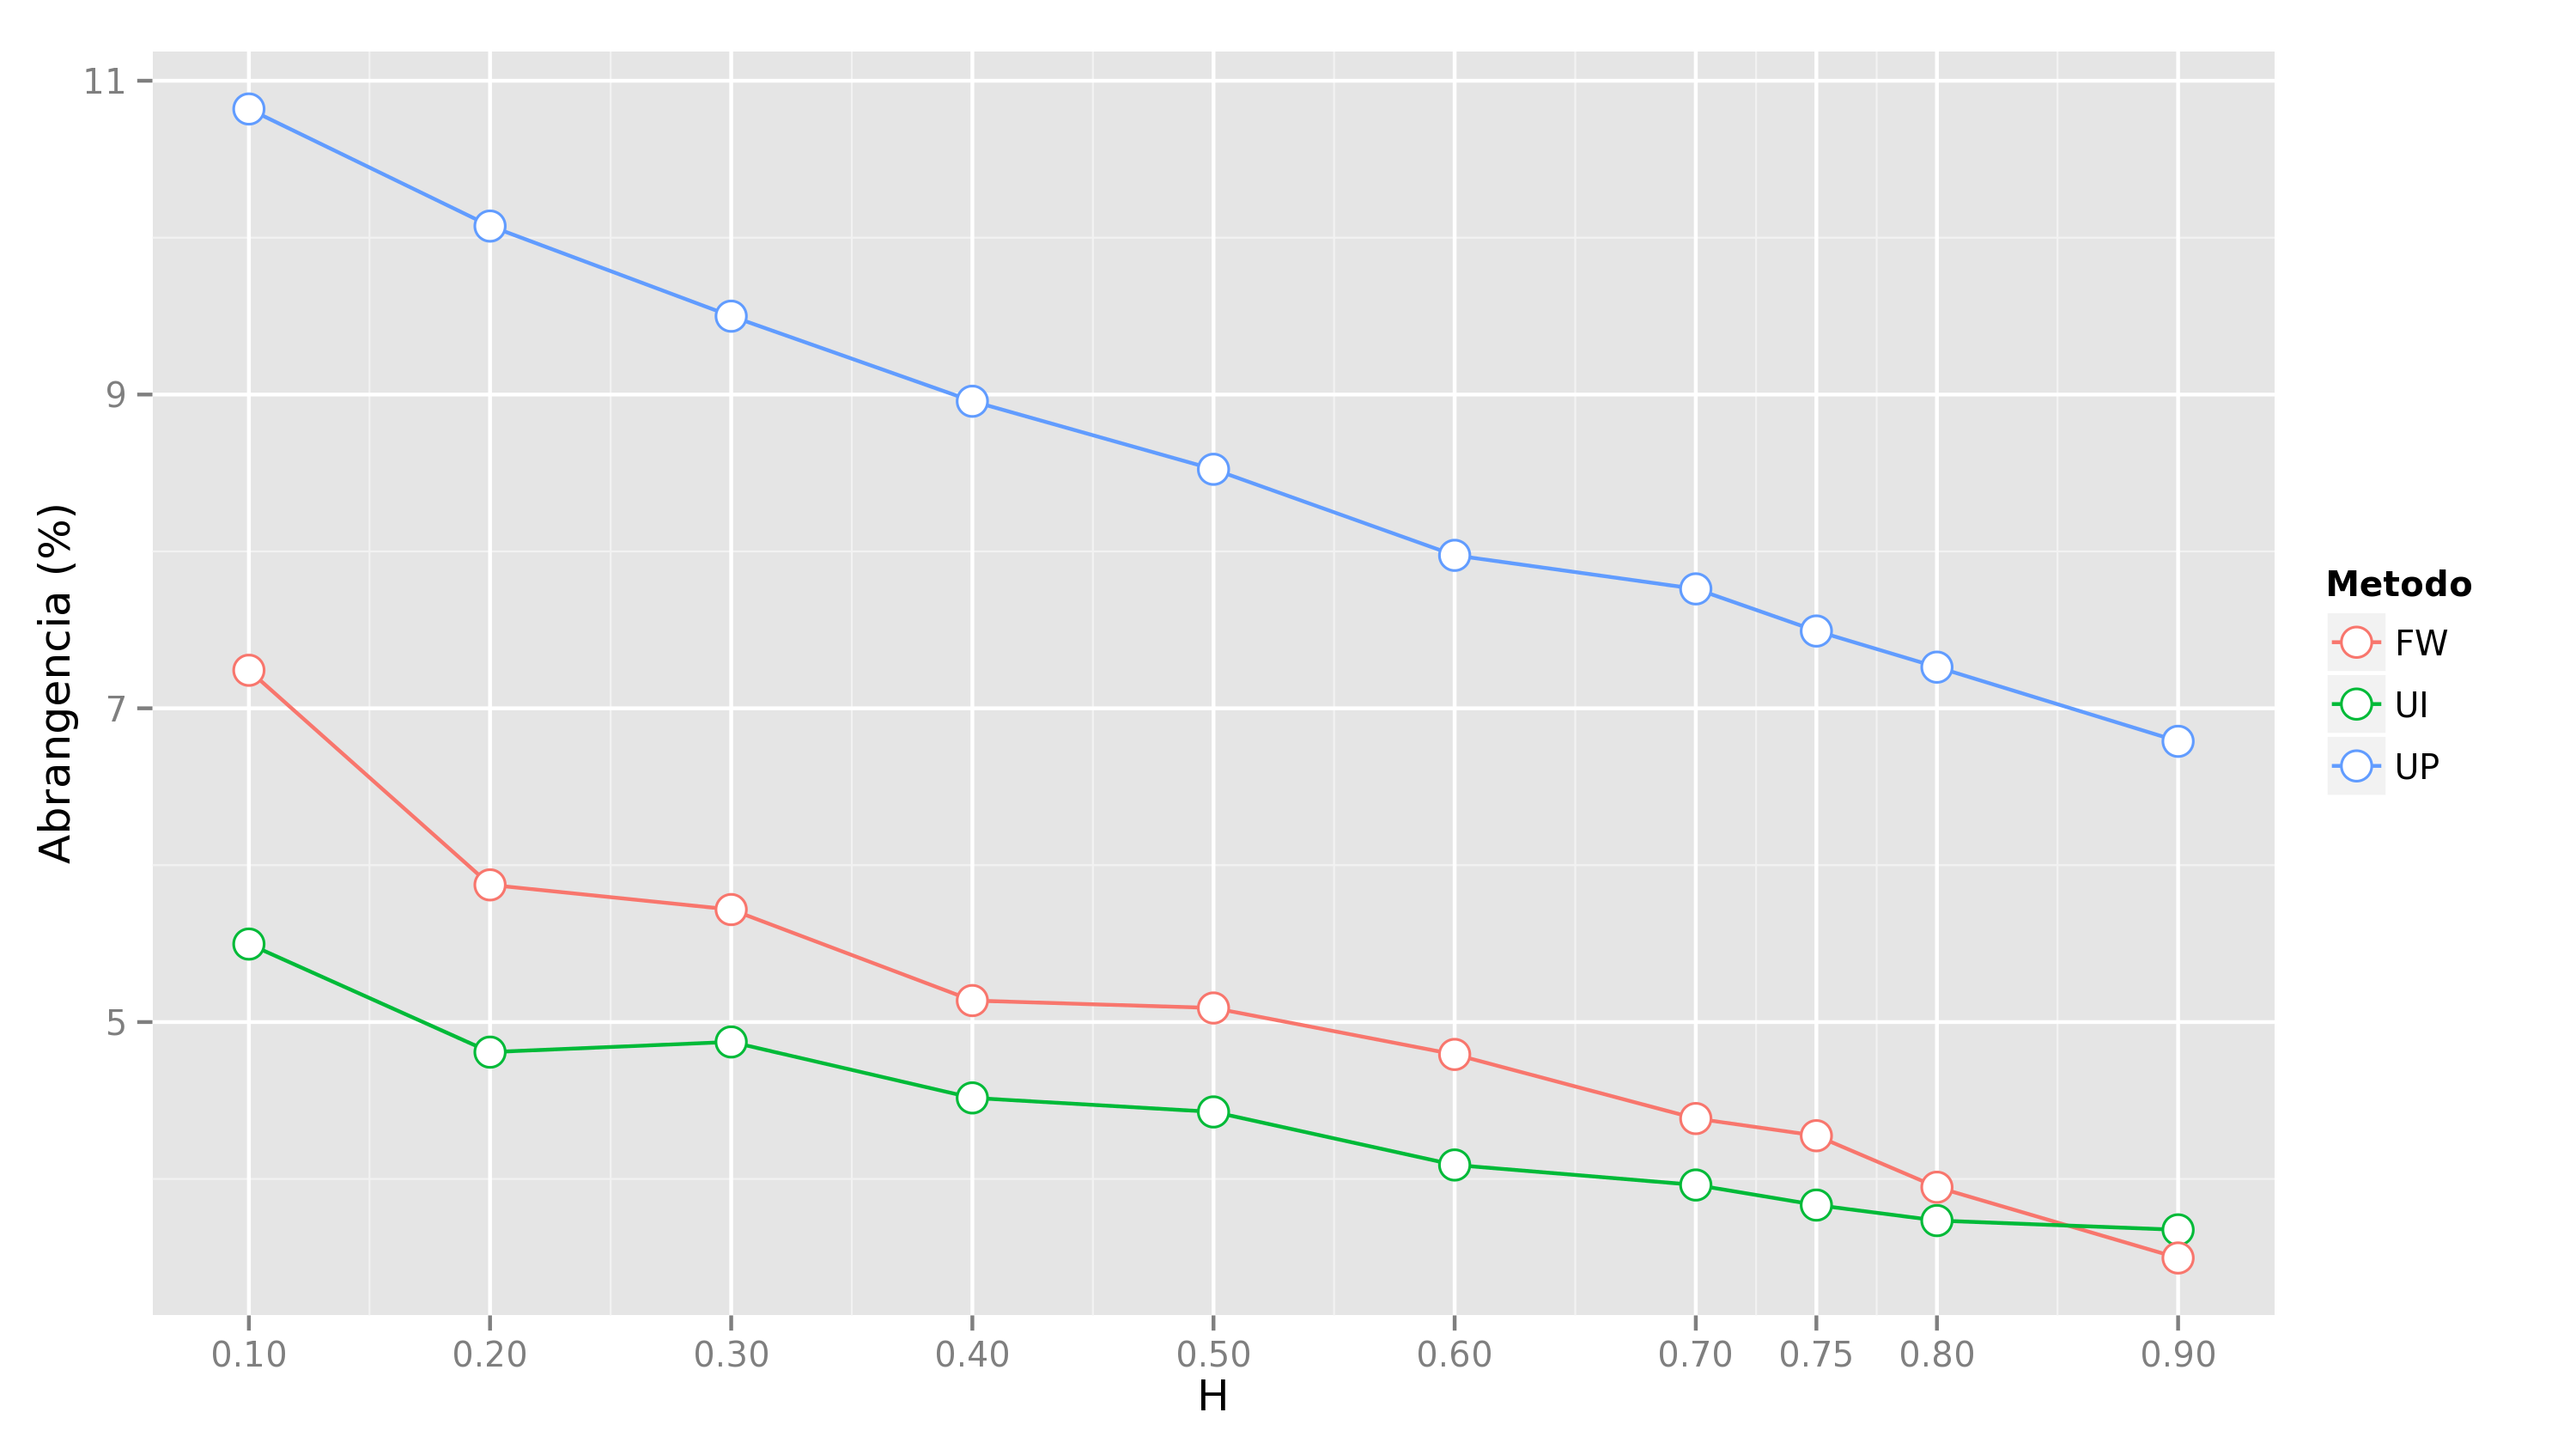
\includegraphics[width=1\textwidth]{img/recall_H}
    \end{center}
    \label{fig:recall_H}
    \caption{Abrangência em função do percentual de avaliações ``escondidas'' $H$}
\end{figure}

\begin{figure}[htp]
    \begin{center}
    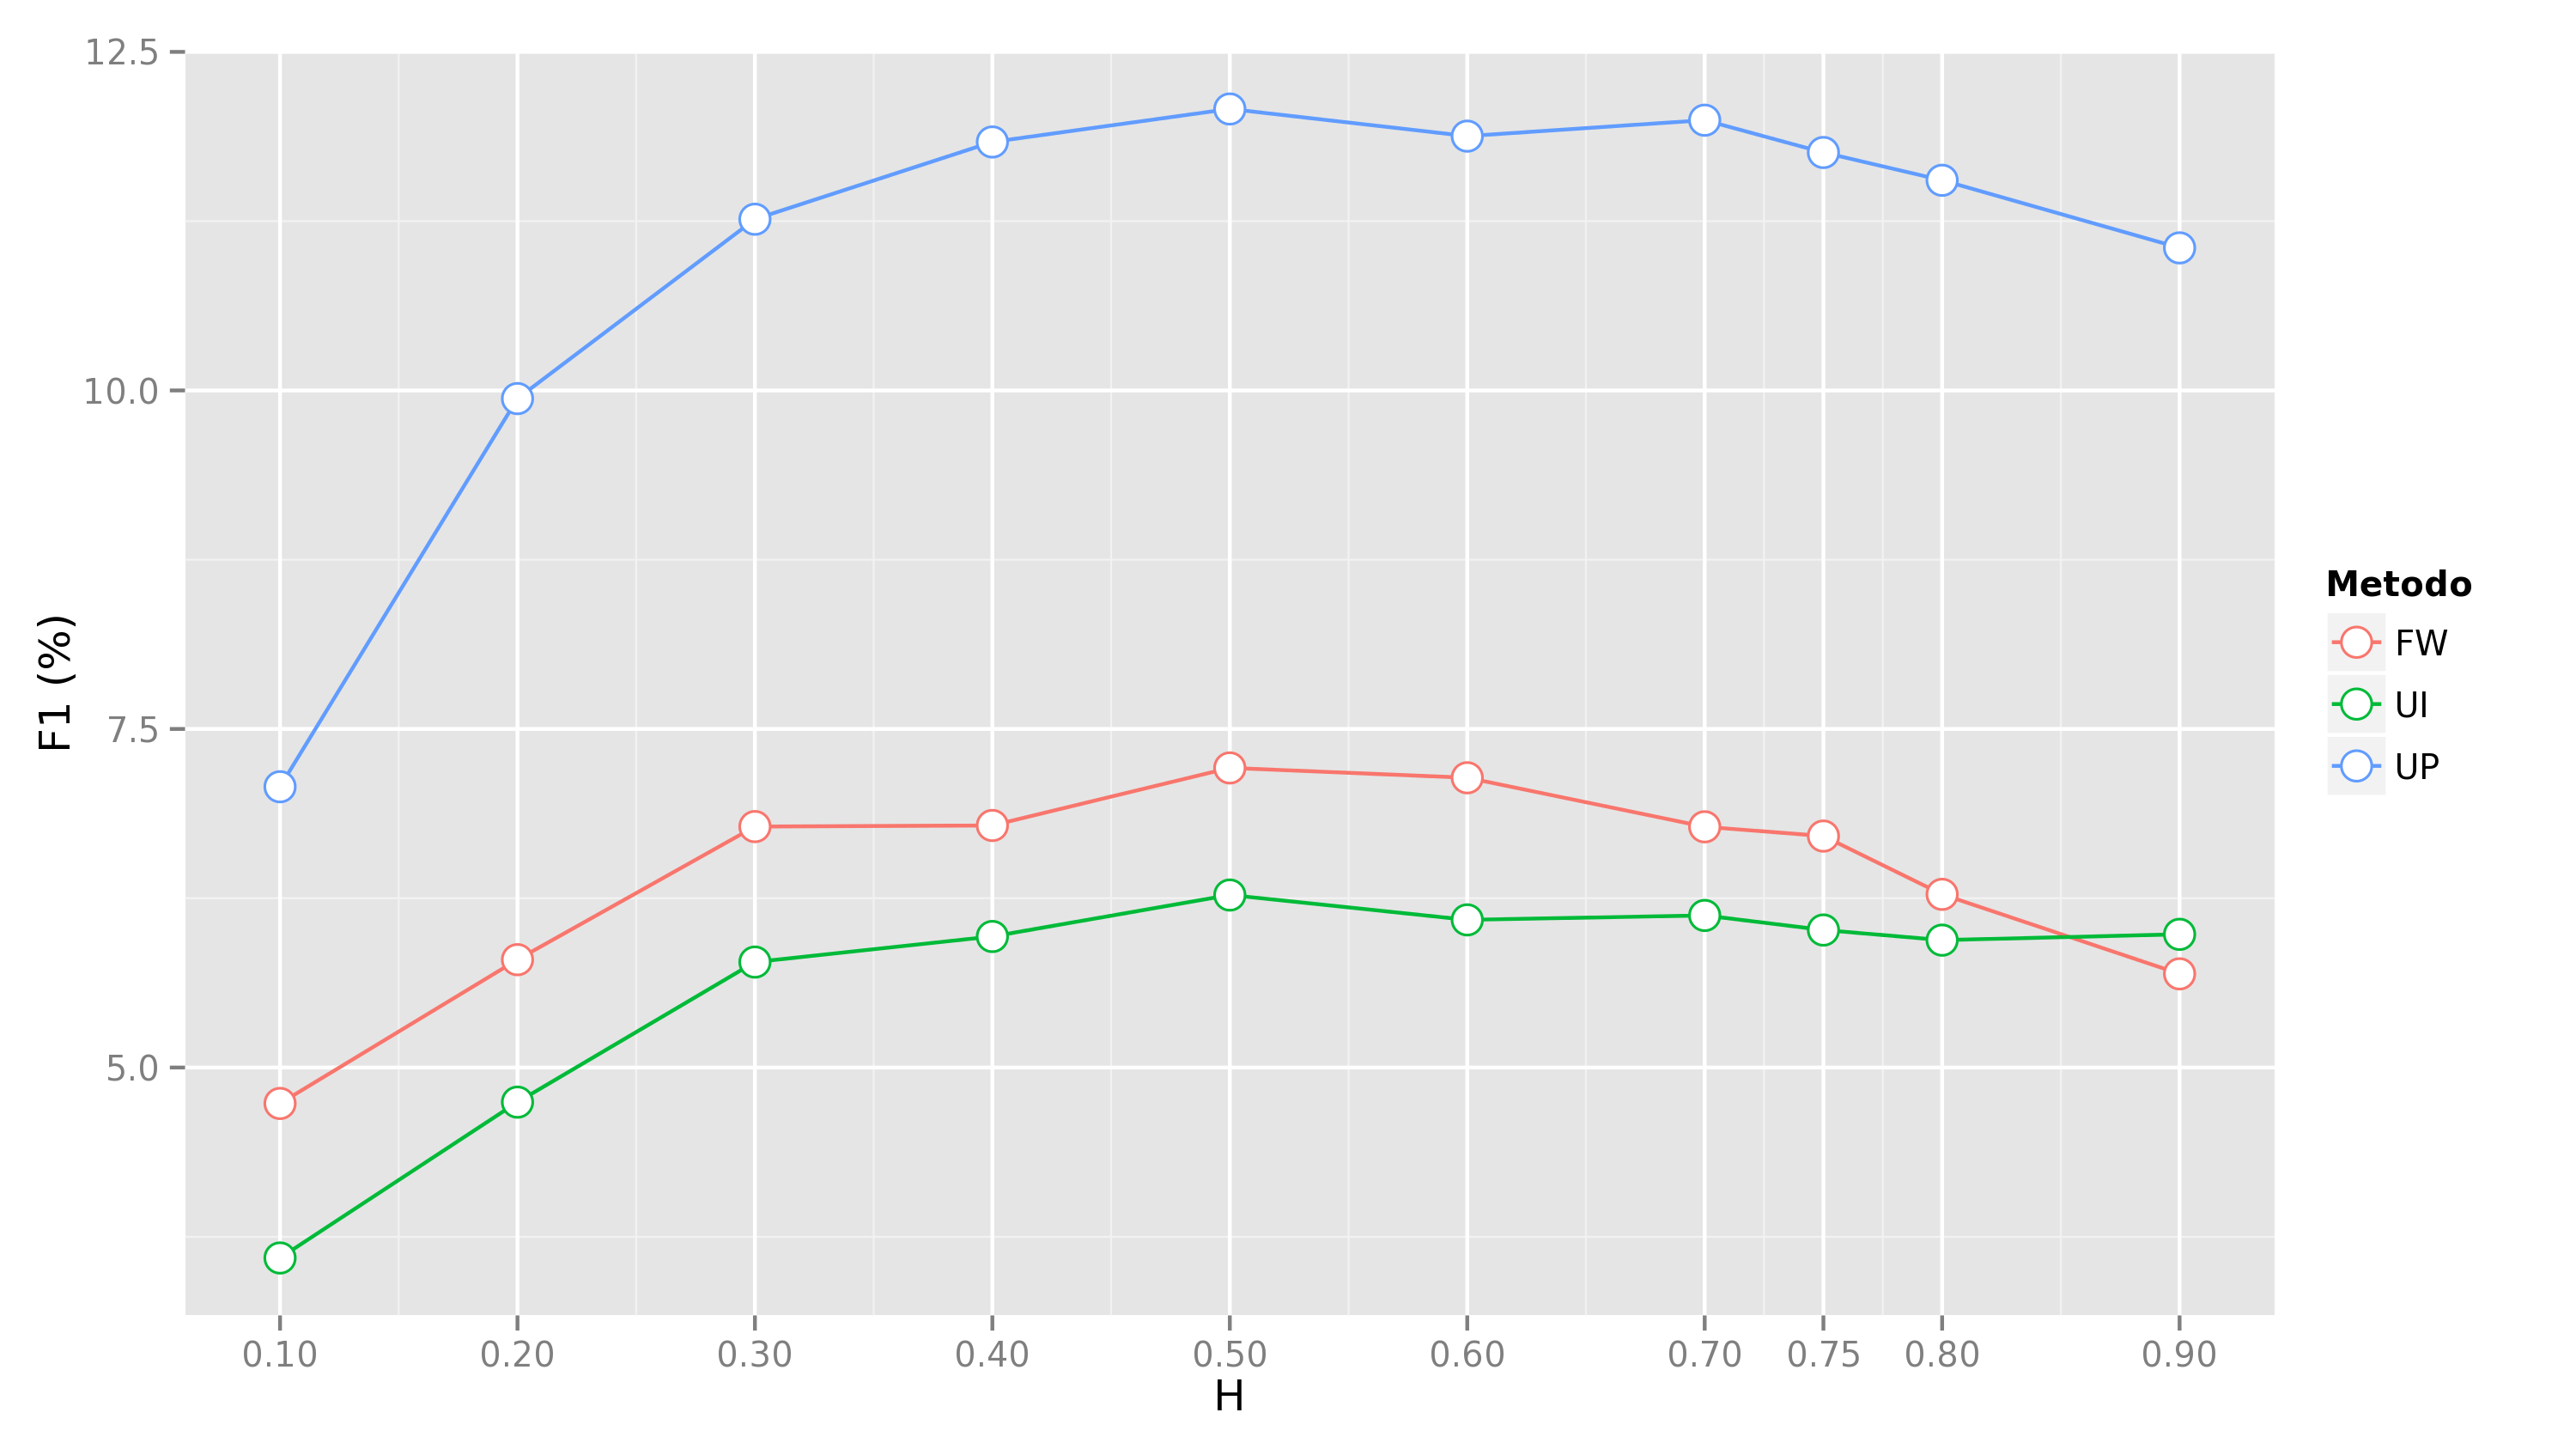
\includegraphics[width=1\textwidth]{img/F1_H}
    \end{center}
    \label{fig:F1_H}
    \caption{Medida $F_1$ em função do percentual de avaliações ``escondidas'' $H$}
\end{figure}

\begin{figure}[htp]
    \begin{center}
    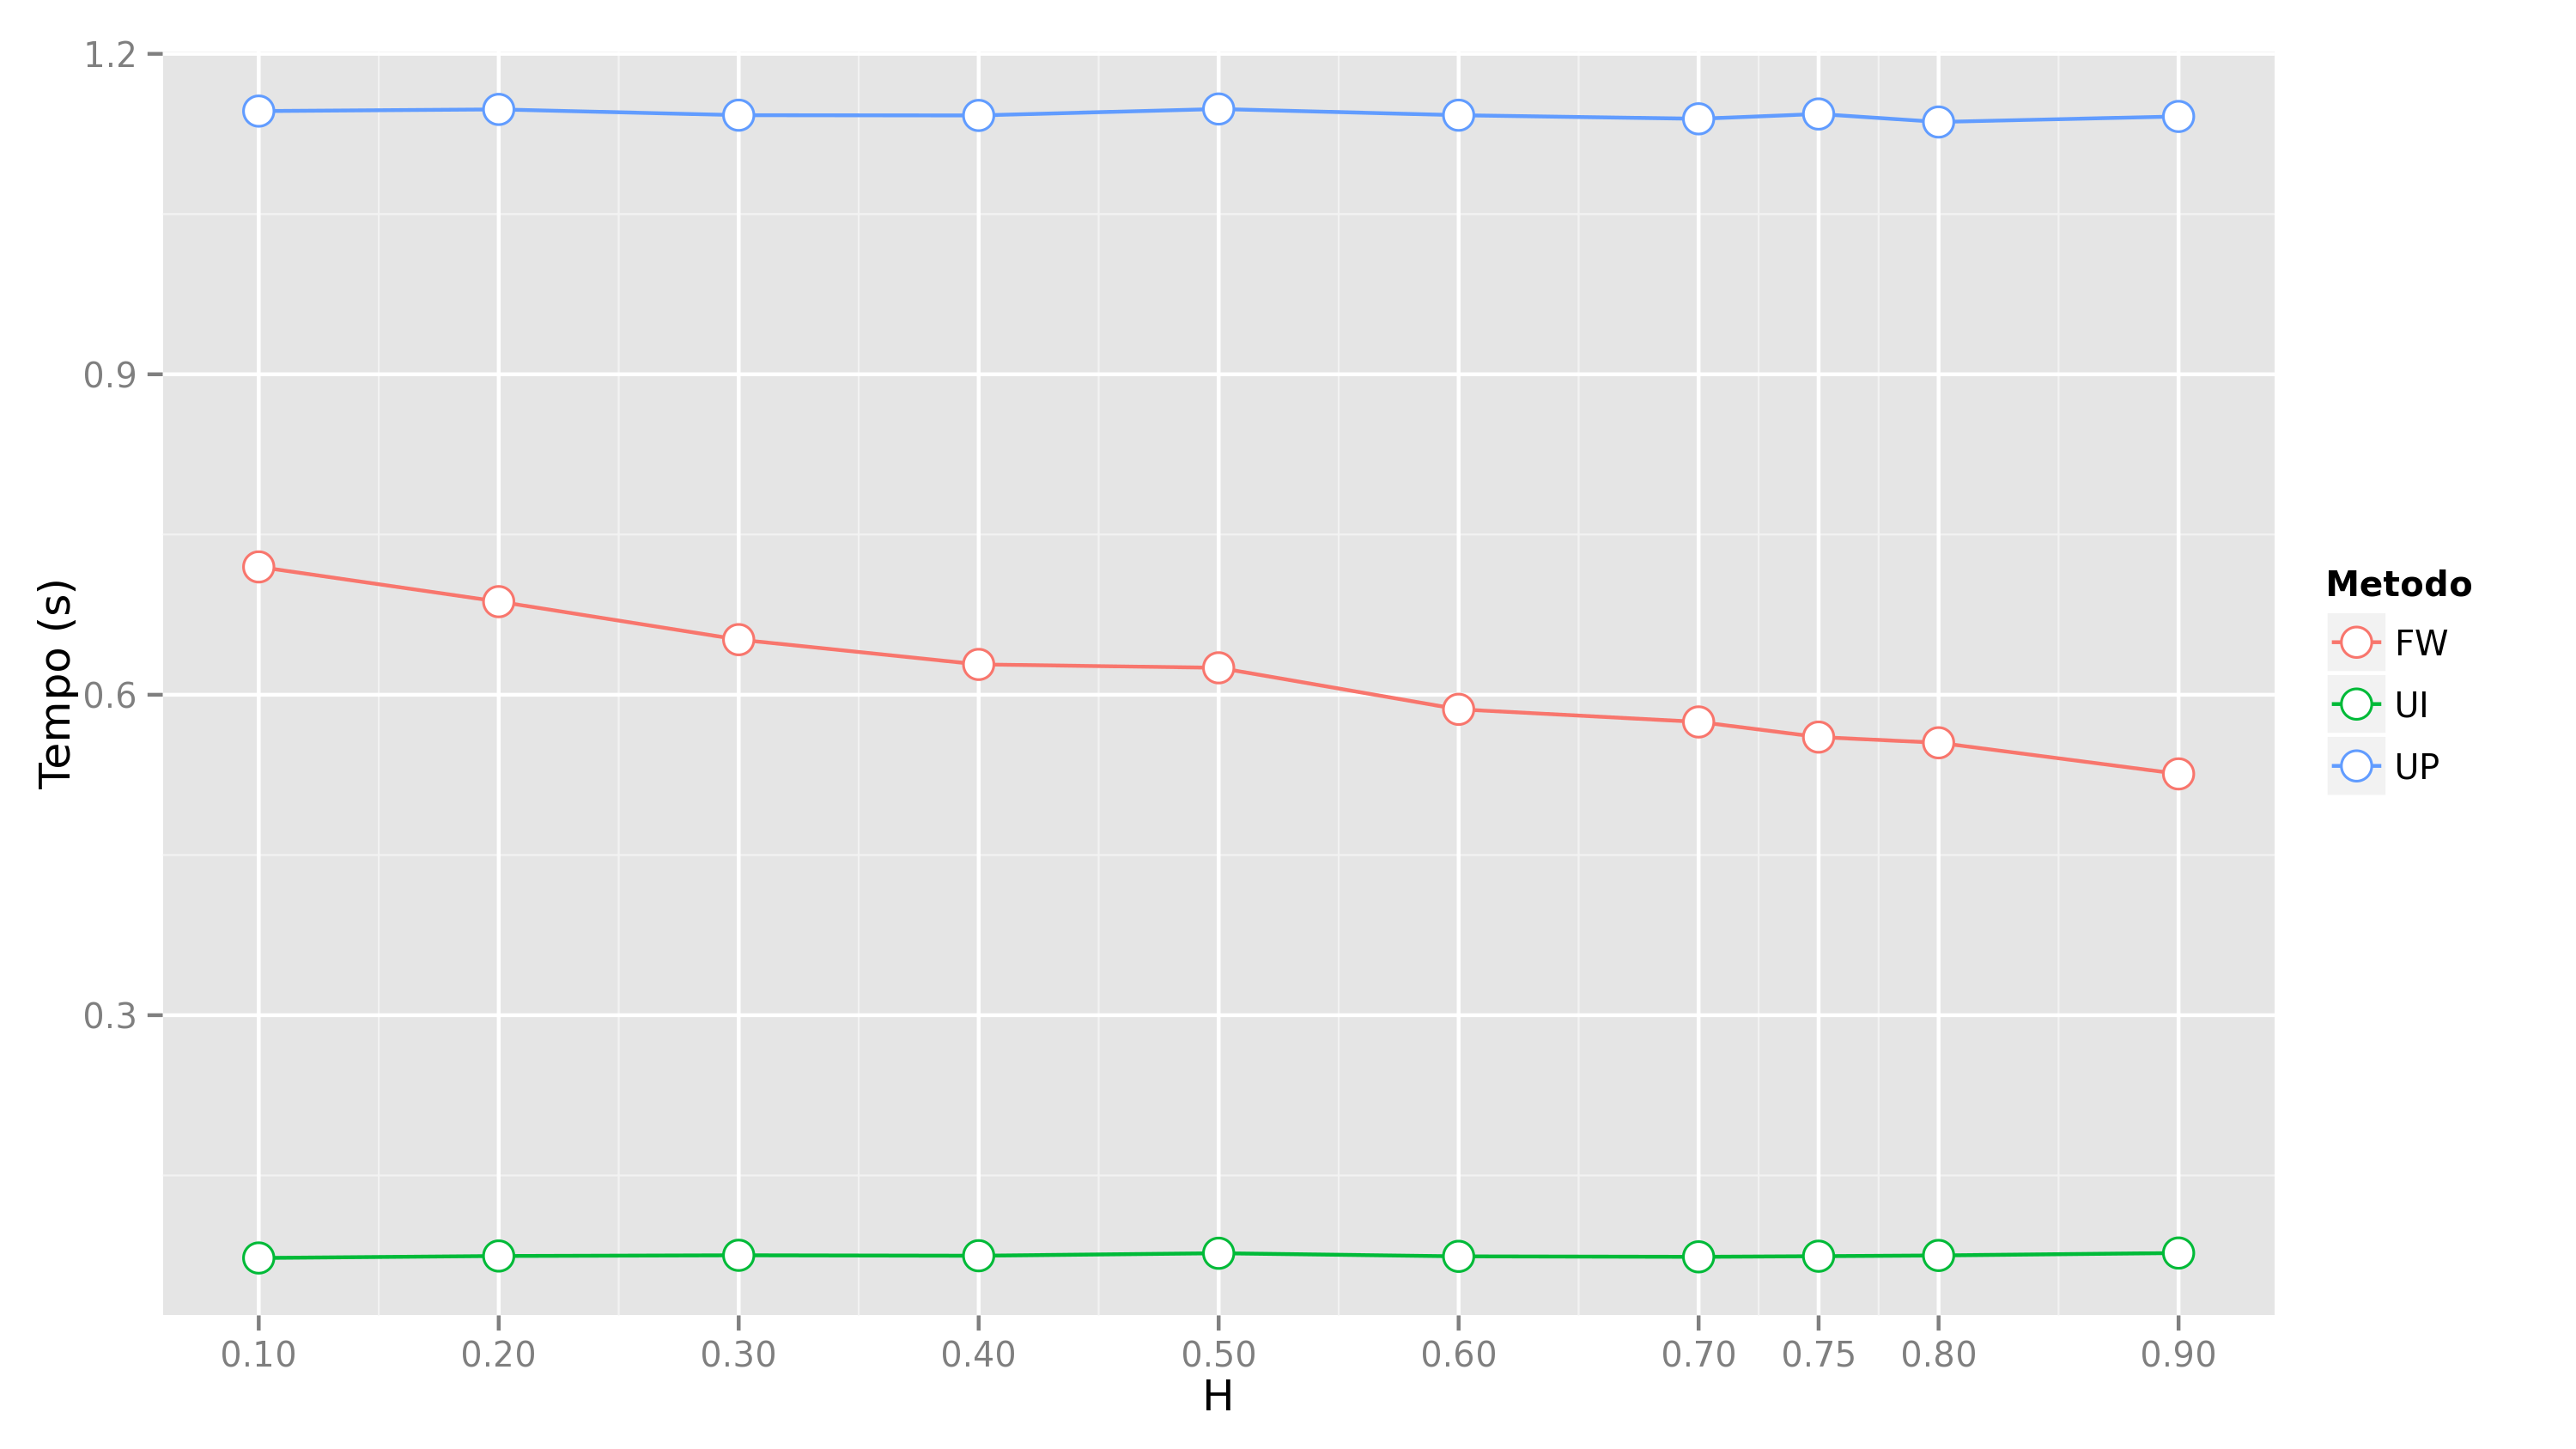
\includegraphics[width=1\textwidth]{img/time_H}
    \end{center}
    \label{fig:time_H}
    \caption{Tempo de execução em função do percentual de avaliações ``escondidas'' $H$}
\end{figure}


\section{Valor mínimo para avaliações positivas $M$} % (fold)
\label{sec:valor_m_nimo_para_avalia_es_positivas_}

Contrariamente ao que esperávamos, tornar o algoritmo mais ``seletivo'' não melhora sua precisão. Apesar de o valor mínimo $M$ estar intimamente ligado com a noção de ``avaliação positiva'' e de entrar no cálculo de parâmetros importantes dos métodos (Equações \ref{eq:determinacao-eij} e \ref{eq:tf}), esse parâmetro pouco influencia a precisão para $0 \leq M \leq 2$. 

Esse resultado pode ser explicado pelo fato de que a maioria das avaliações são positivas (Figura \ref{fig:percentual_M}), e portanto $\mathrm{b}_M$ tem quase o mesmo efeito de $\mathrm{b}_0$. Isso não ocorre somente pelo fato de os clientes comprarem itens similares a seus gostos, e portanto de raramente se decepcionarem, mas também pelo fato de que os usuários tem menos disposição para darem avaliações negativas. Esse fenômeno se chama \textit{hidden feedback}, e se caracteriza pelo fato de que os itens avaliados não são escolhidos ao acaso, mas sim por despertarem aspectos de interesse das preferências do usuário, indo além dos valores numéricos das avaliações \cite{lops2011content-chap5}.

Ao se analisar a abrangência dos métodos, a seletividade influencia na recomendação. Quanto maior $M$, menor é a quantidade de itens muito bem avaliados. Estes possuem elevada similaridade-correlação e são facilmente escolhidos pelos algoritmos. Por esse motivo, melhor é o desempenho do sistema.

A complexidade computacional dos algoritmos também depende de $M$, já que mais ou menos parâmetros são analisados no cálculo da TF-IDF (métodos UI e UP) e dos pesos dos atributos (método FW).

Um detalhe a se observar é que a precisão é nula e a abrangência é inexistente para $M=5$, já que todas as avaliações $r_{ui}$ pertencem ao conjunto $\left\{1,2,3,4,5\right\}$. 
Para o algoritmo UI, tanto a precisão quanto a abrangência são nulas para $M=4$.

\begin{figure}[htp]
    \begin{center}
    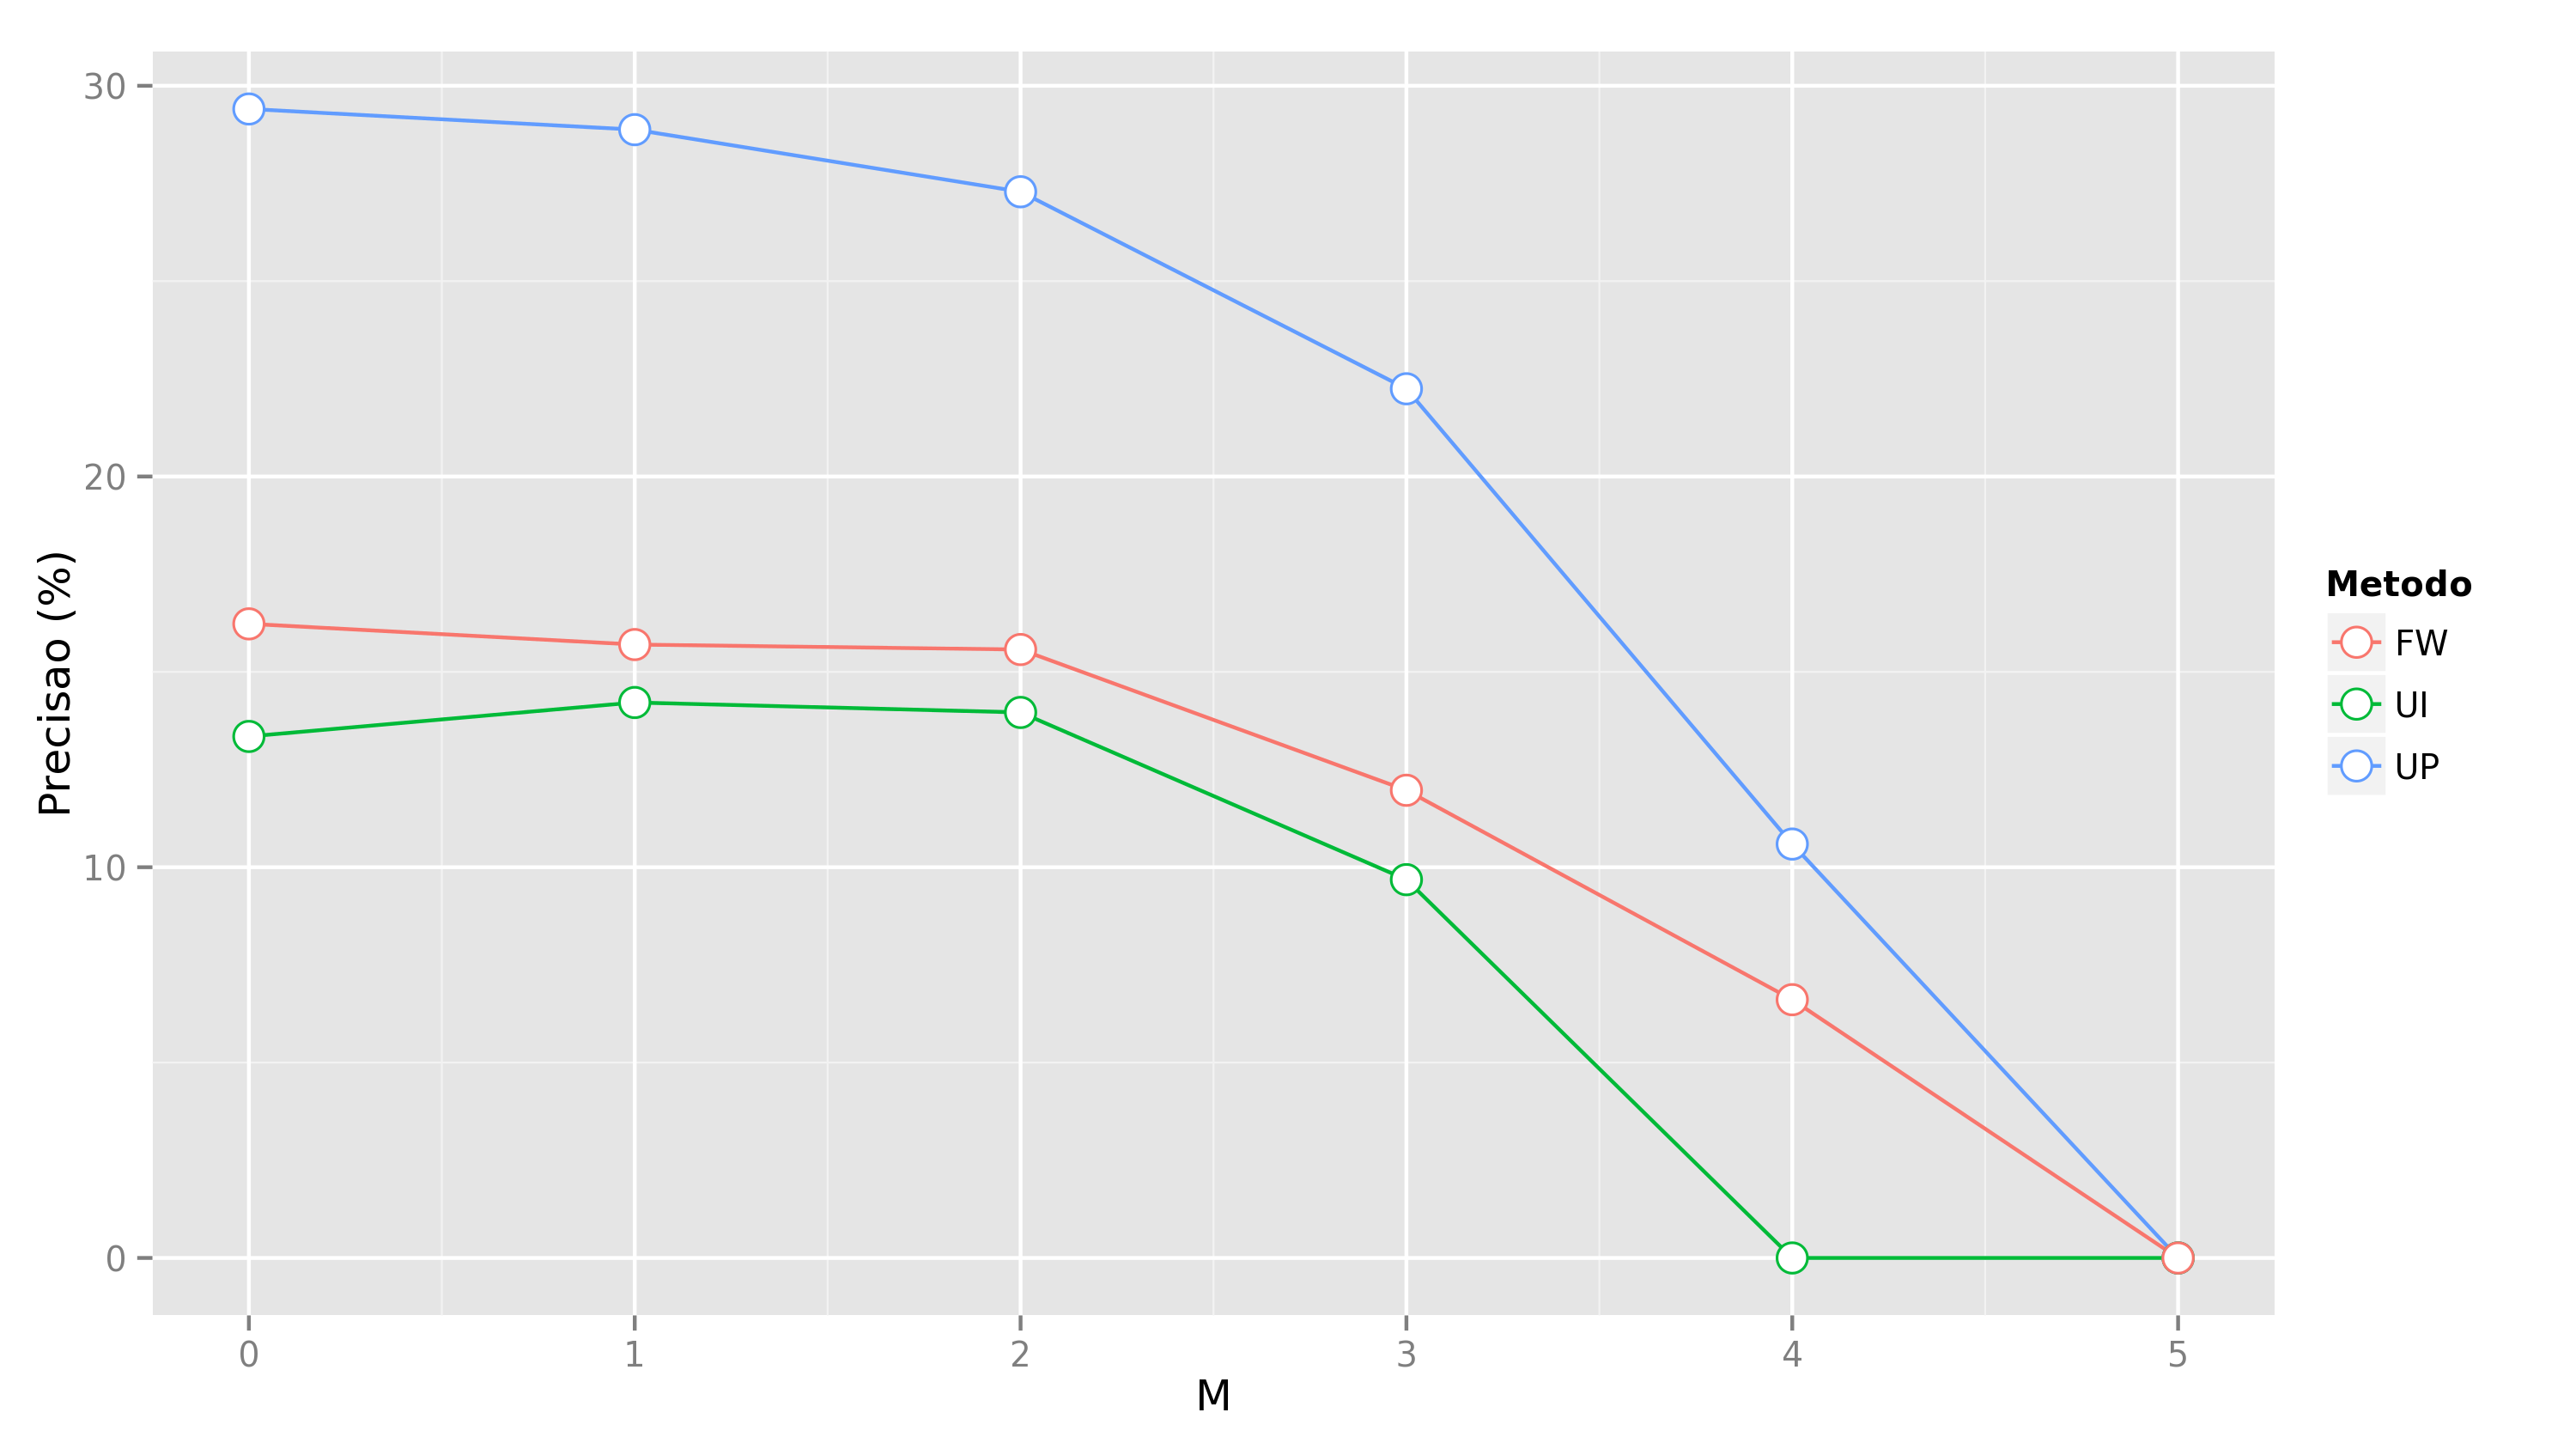
\includegraphics[width=1\textwidth]{img/precision_M}
    \end{center}
    \label{fig:precision_M}
    \caption{Precisão em função do valor mínimo para avaliações positivas $M$}
\end{figure}

\begin{figure}[htp]
    \begin{center}
    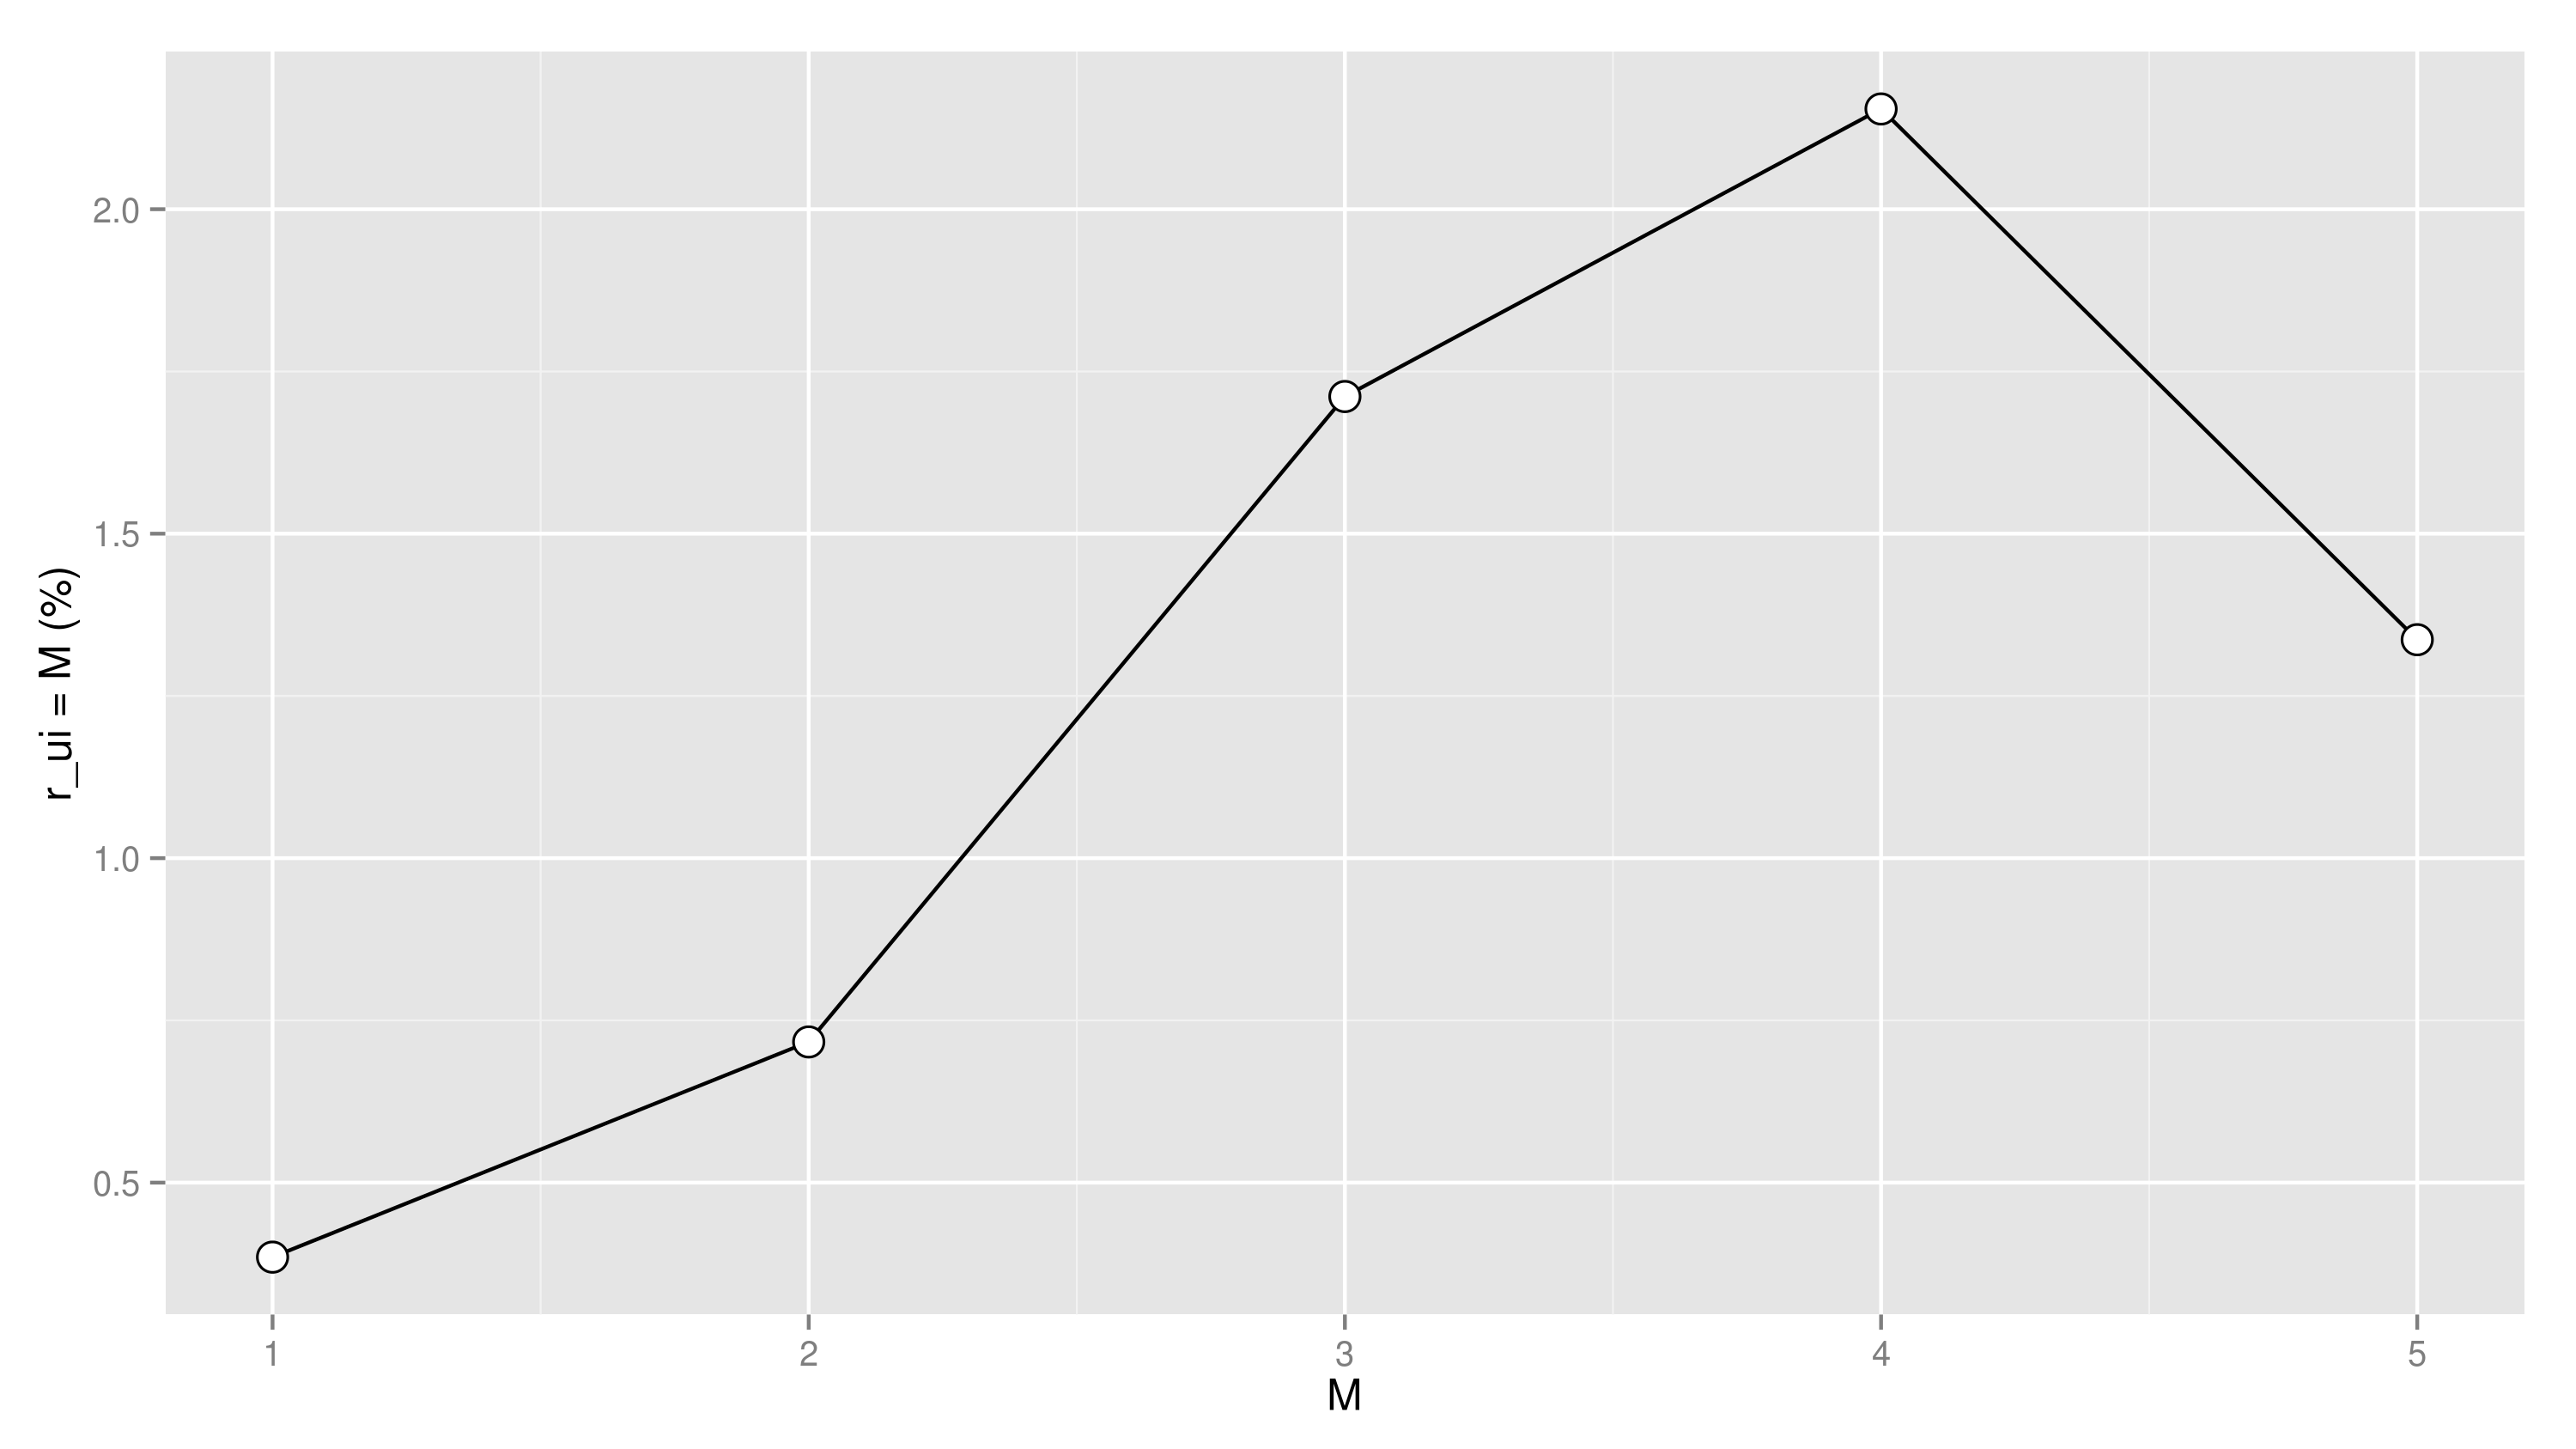
\includegraphics[width=1\textwidth]{img/percentual_M}
    \end{center}
    \label{fig:percentual_M}
    \caption{Percentual de avaliações por valor de $M$}
\end{figure}

\begin{figure}[htp]
    \begin{center}
    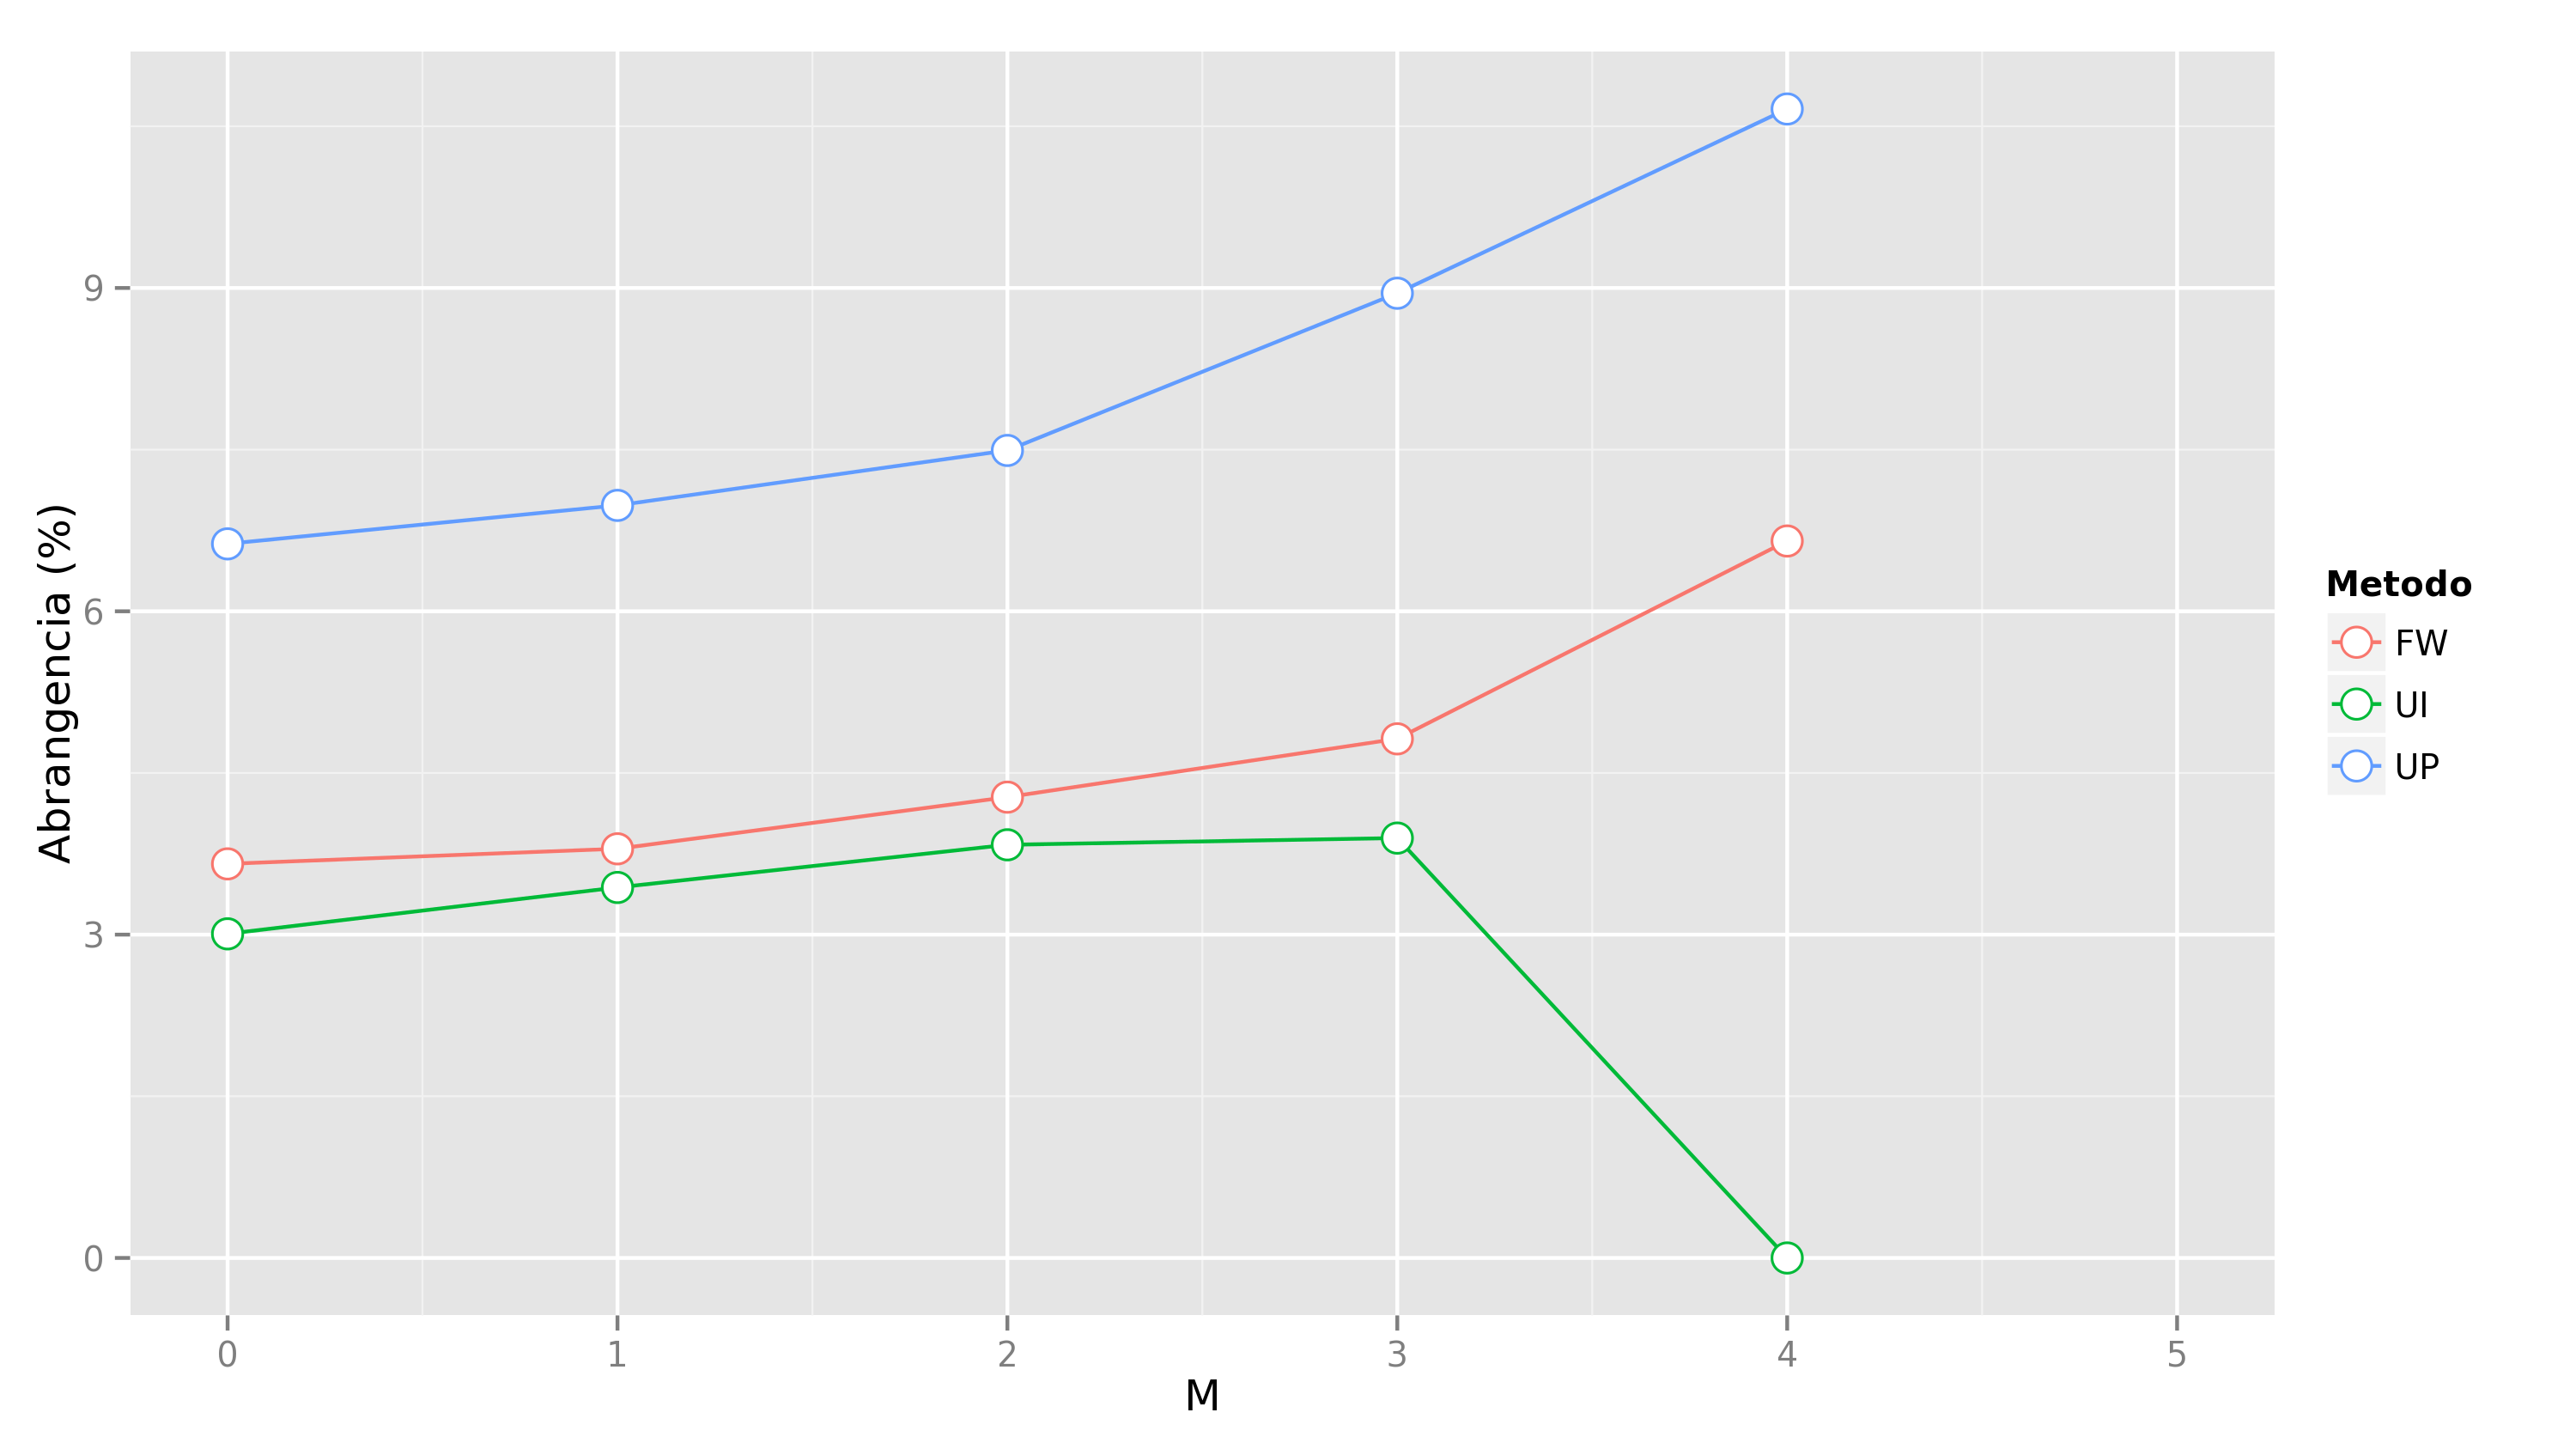
\includegraphics[width=1\textwidth]{img/recall_M}
    \end{center}
    \label{fig:recall_M}
    \caption{Abrangência em função do valor mínimo para avaliações positivas $M$}
\end{figure}

\begin{figure}[htp]
    \begin{center}
    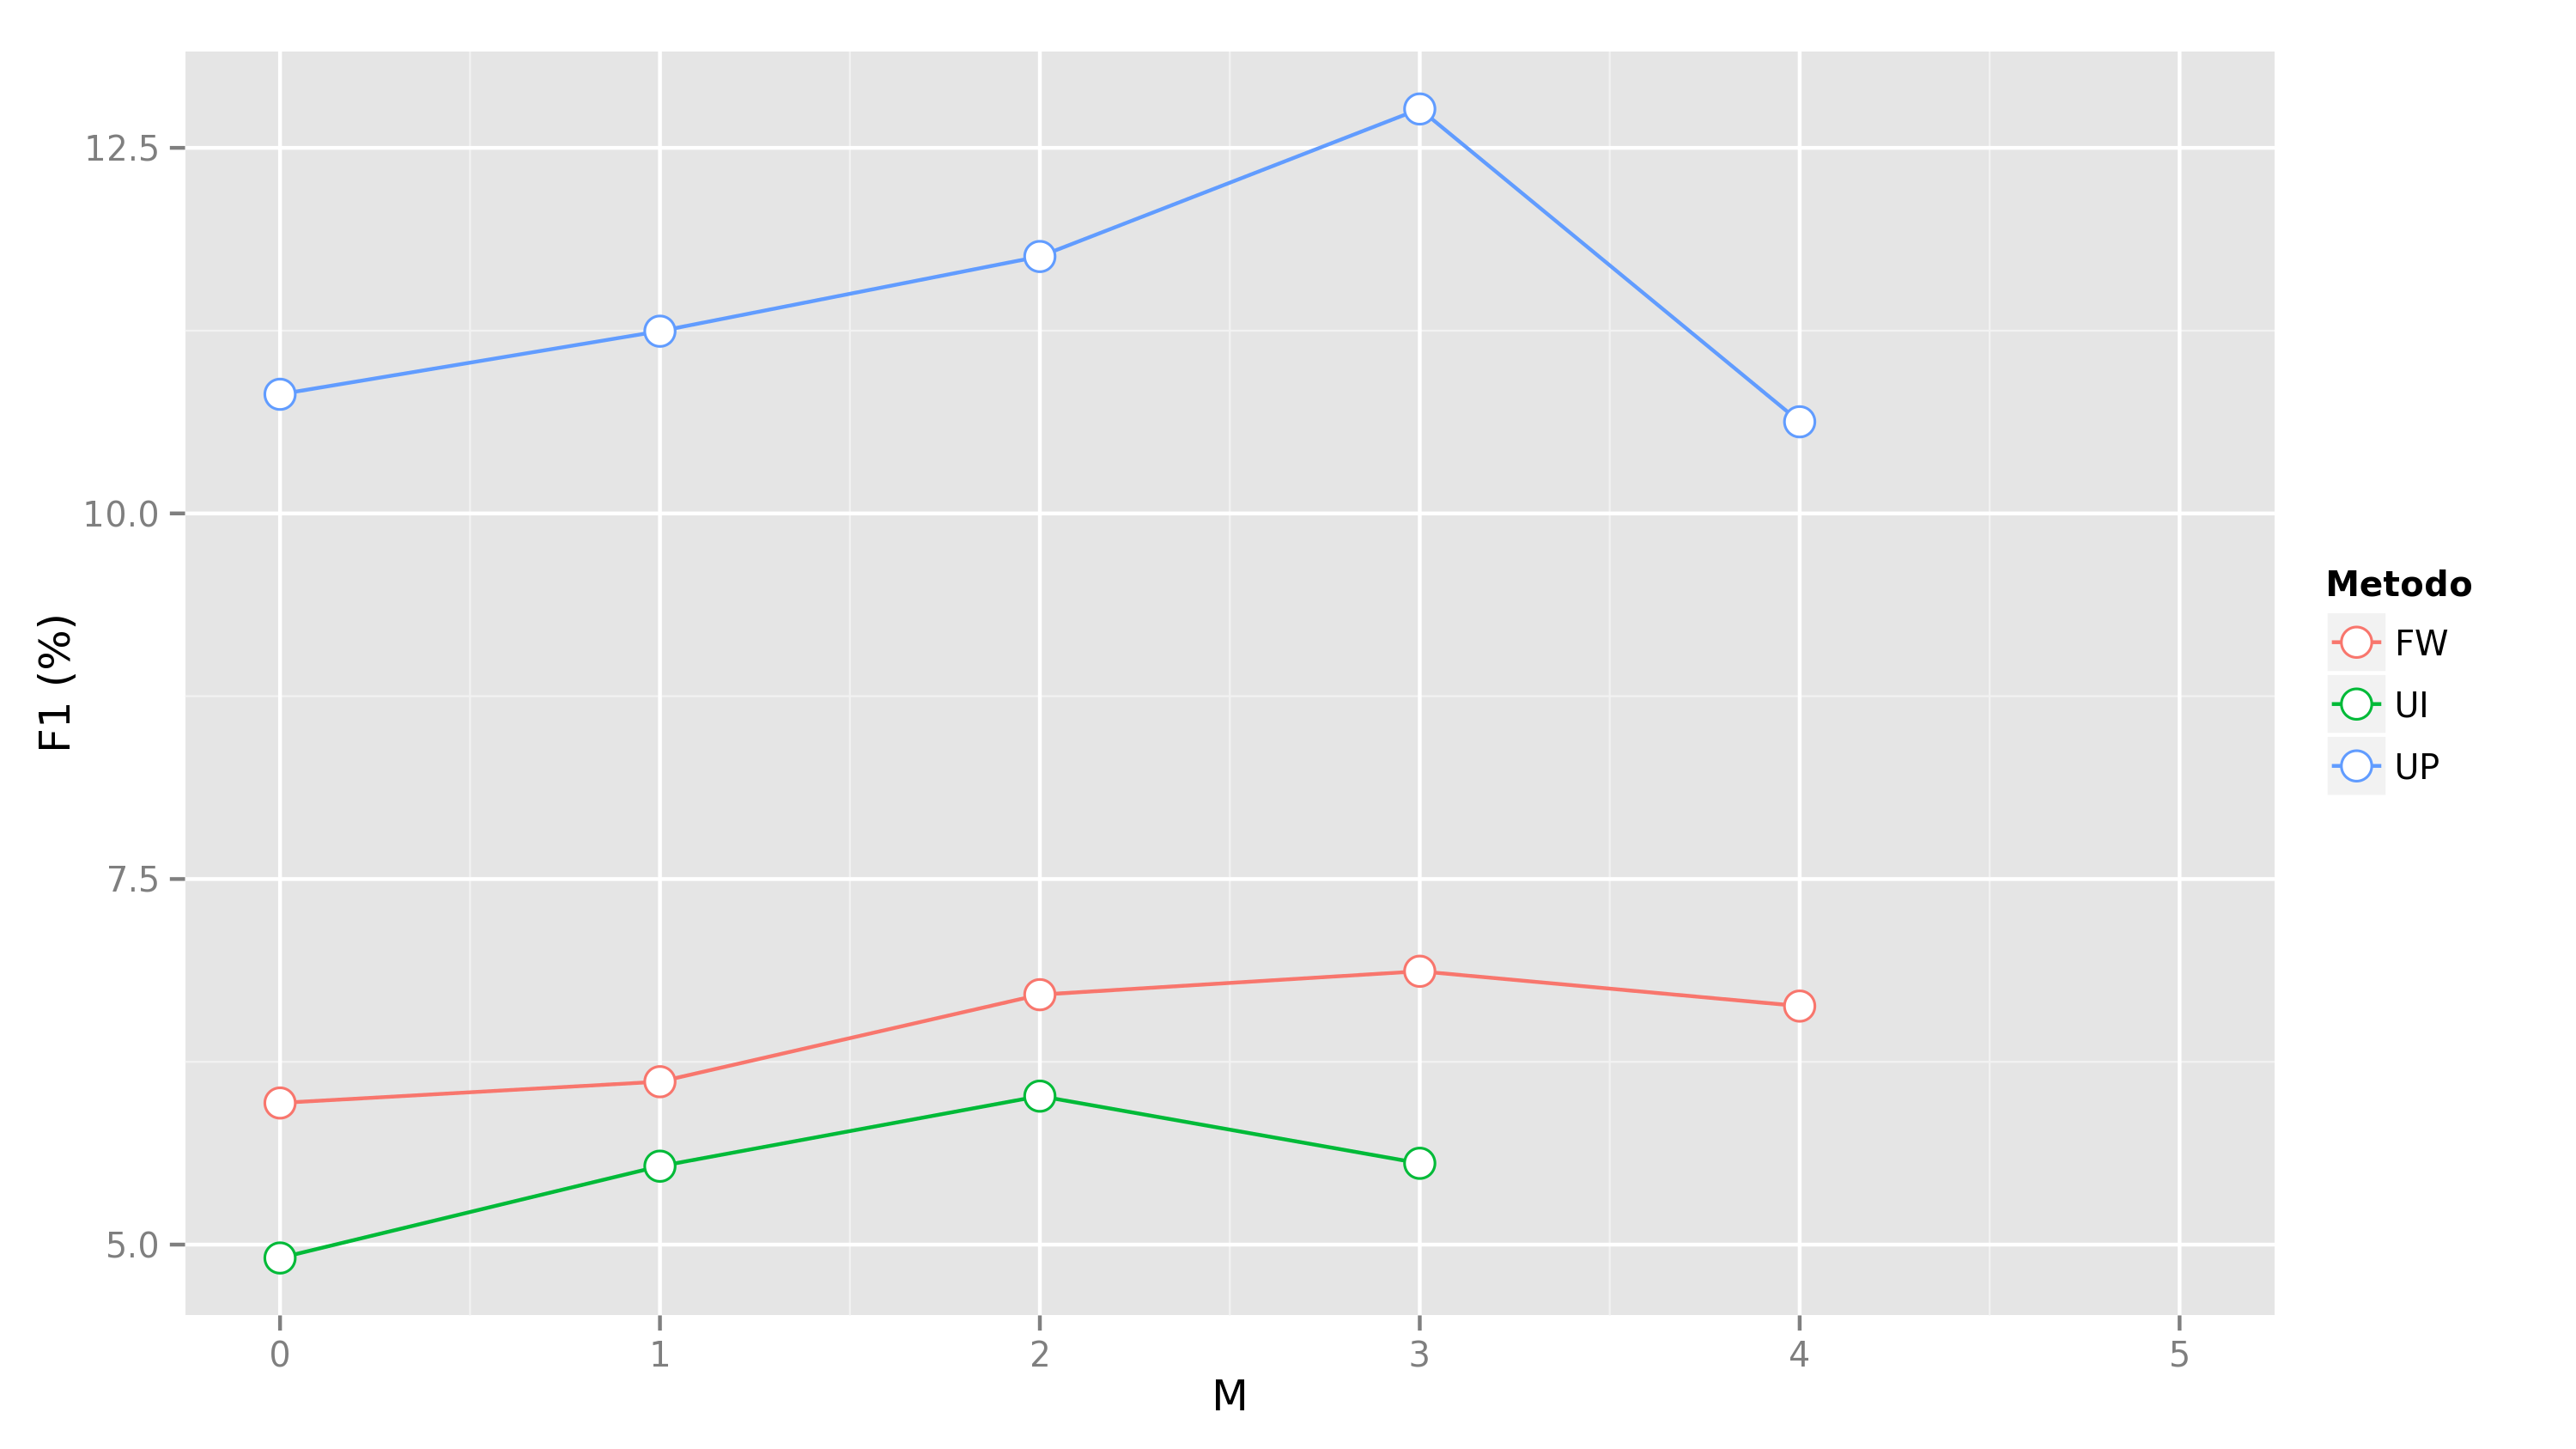
\includegraphics[width=1\textwidth]{img/F1_M}
    \end{center}
    \label{fig:F1_M}
    \caption{Medida $F_1$ em função do valor mínimo para avaliações positivas $M$}
\end{figure}

\begin{figure}[htp]
    \begin{center}
    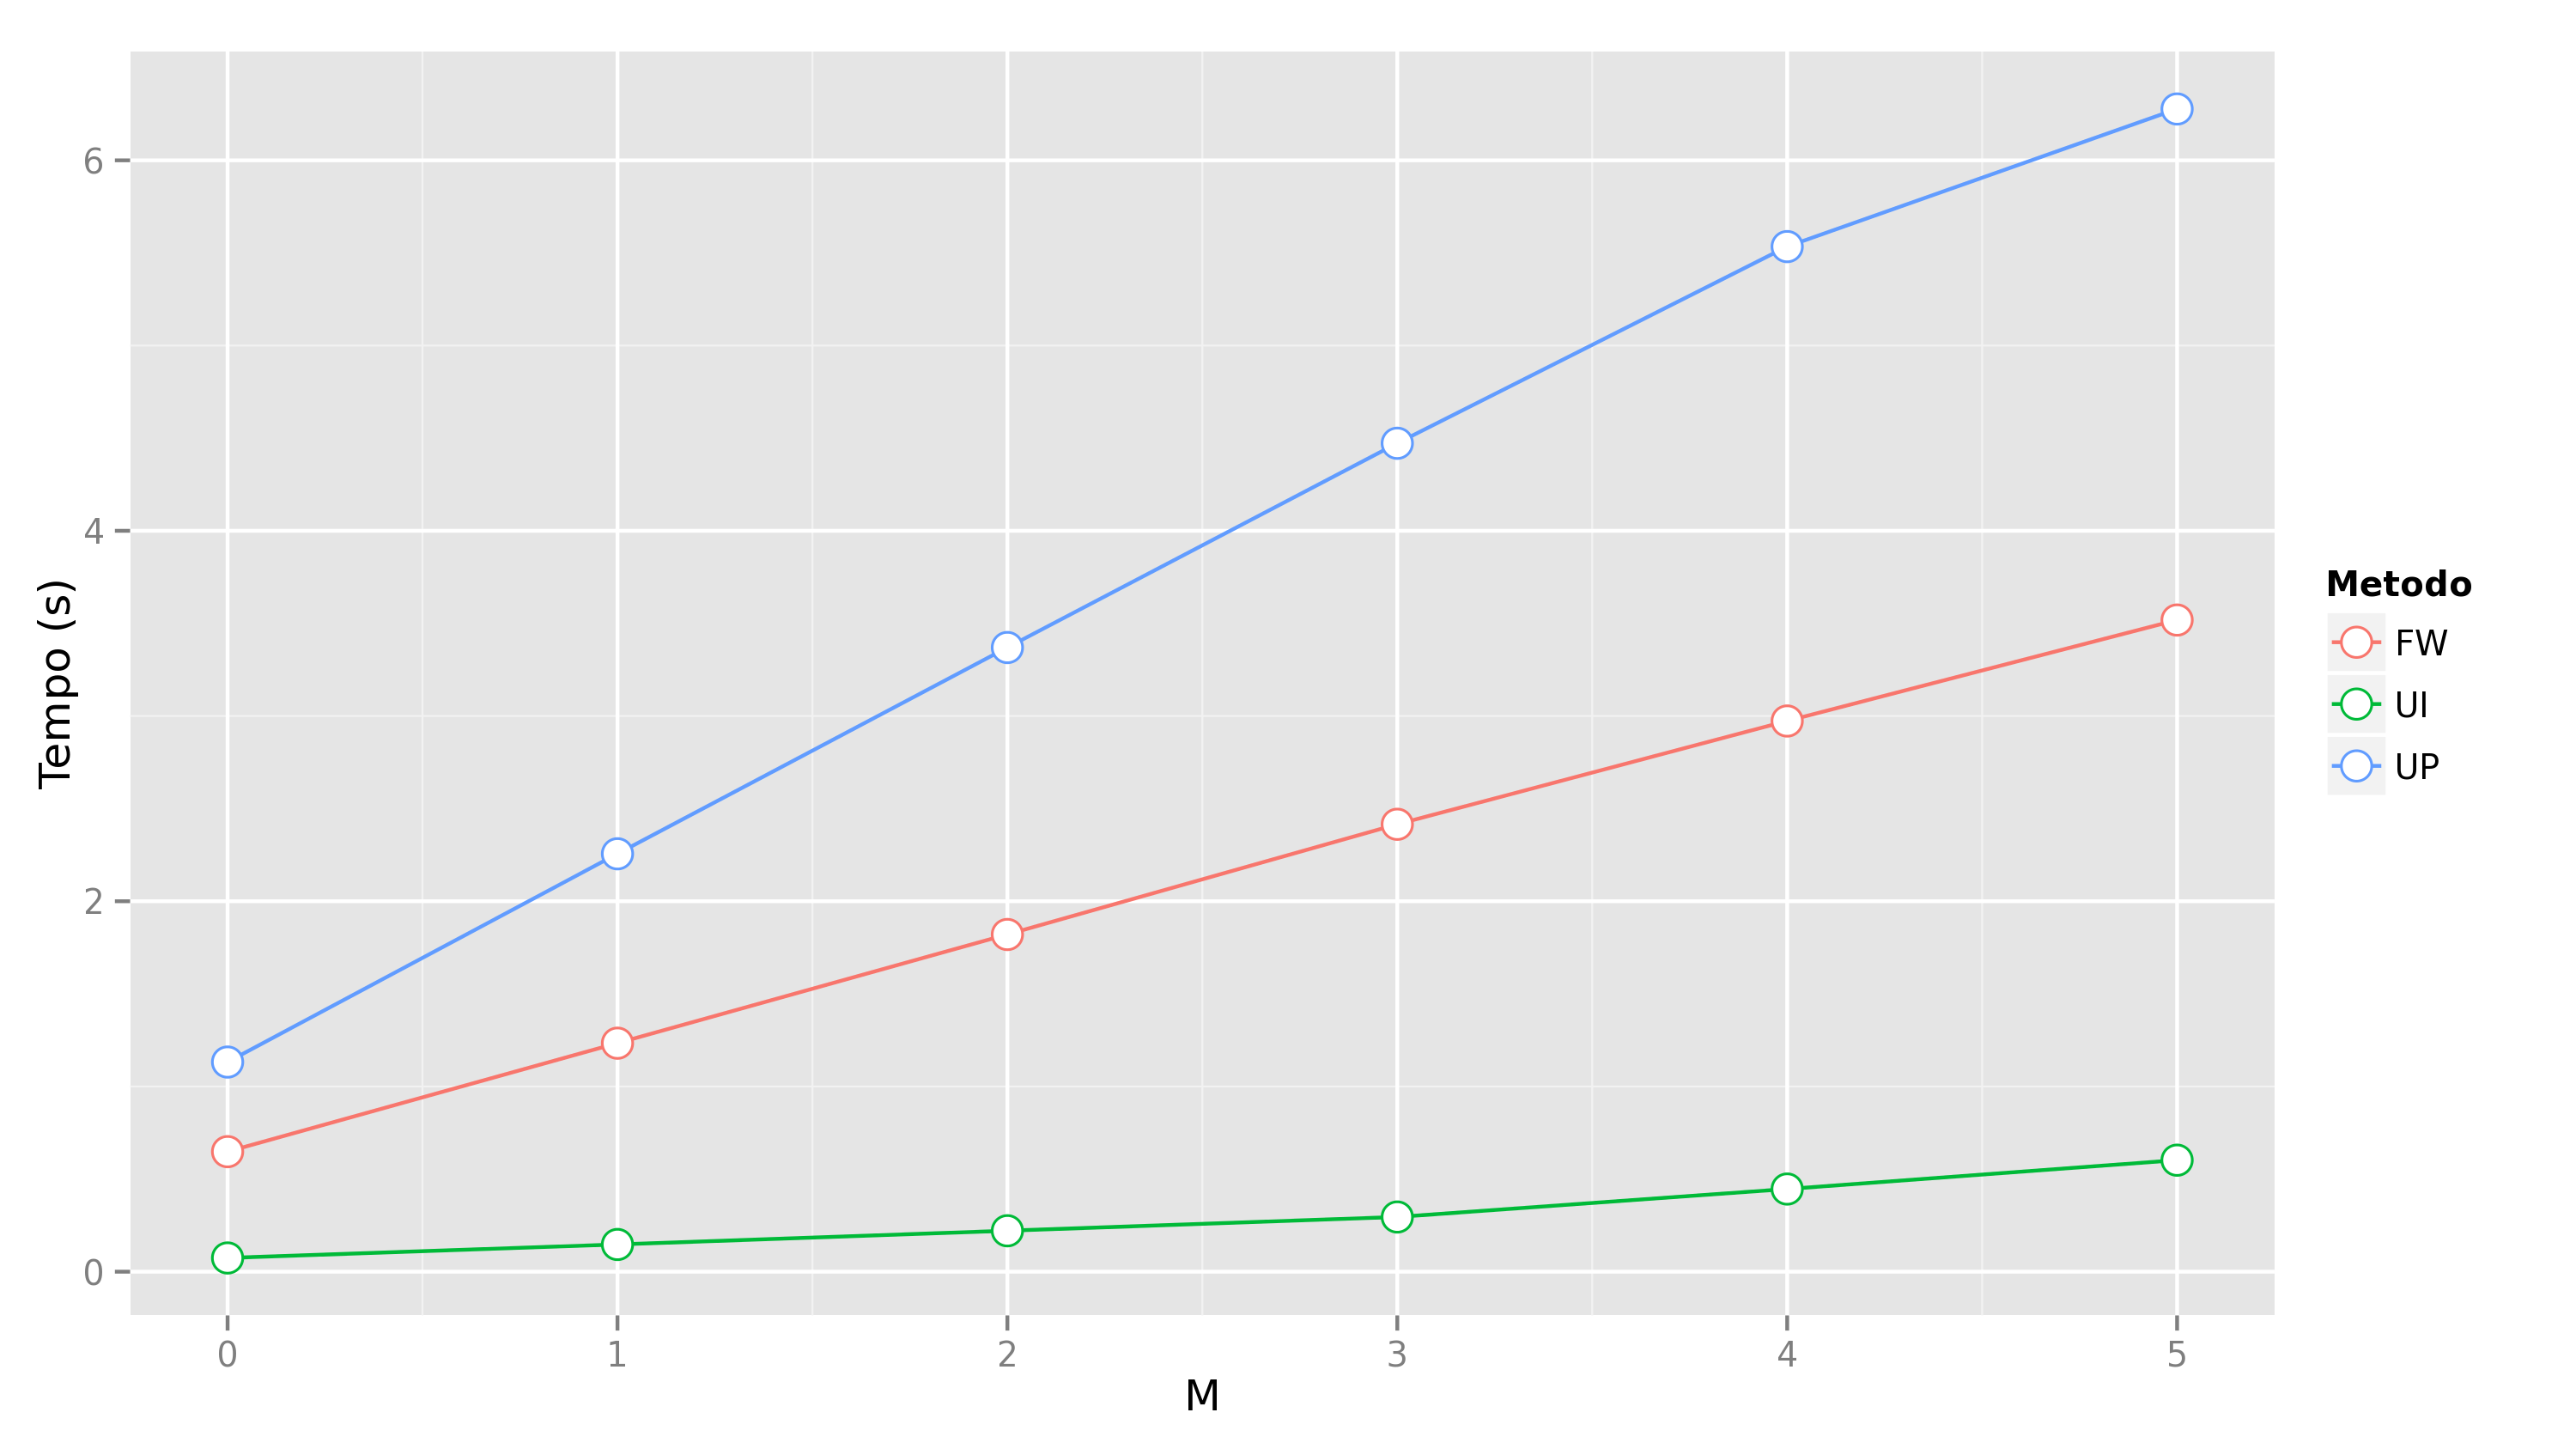
\includegraphics[width=1\textwidth]{img/time_M}
    \end{center}
    \label{fig:time_M}
    \caption{Tempo de execução em função do valor mínimo para avaliações positivas $M$}
\end{figure}

\section{Número de vizinhos mais próximos $k$} % (fold)
\label{sec:n_mero_de_vizinhos_mais_pr_ximos_}

O único método que recomenda itens com base nos vizinhos mais próximos é o UP. Percebe-se que com o aumento de $k$, a precisão e a abrangência caem, pois a vizinhança se torna excessivamente grande e repleta de usuários sem muita similaridade com o usuário-teste. Pode-se observar que o valor máximo de precisão e acurácia ocorre para $k=20$ (Figura \ref{fig:F1_k}).

\begin{figure}[htp]
    \begin{center}
    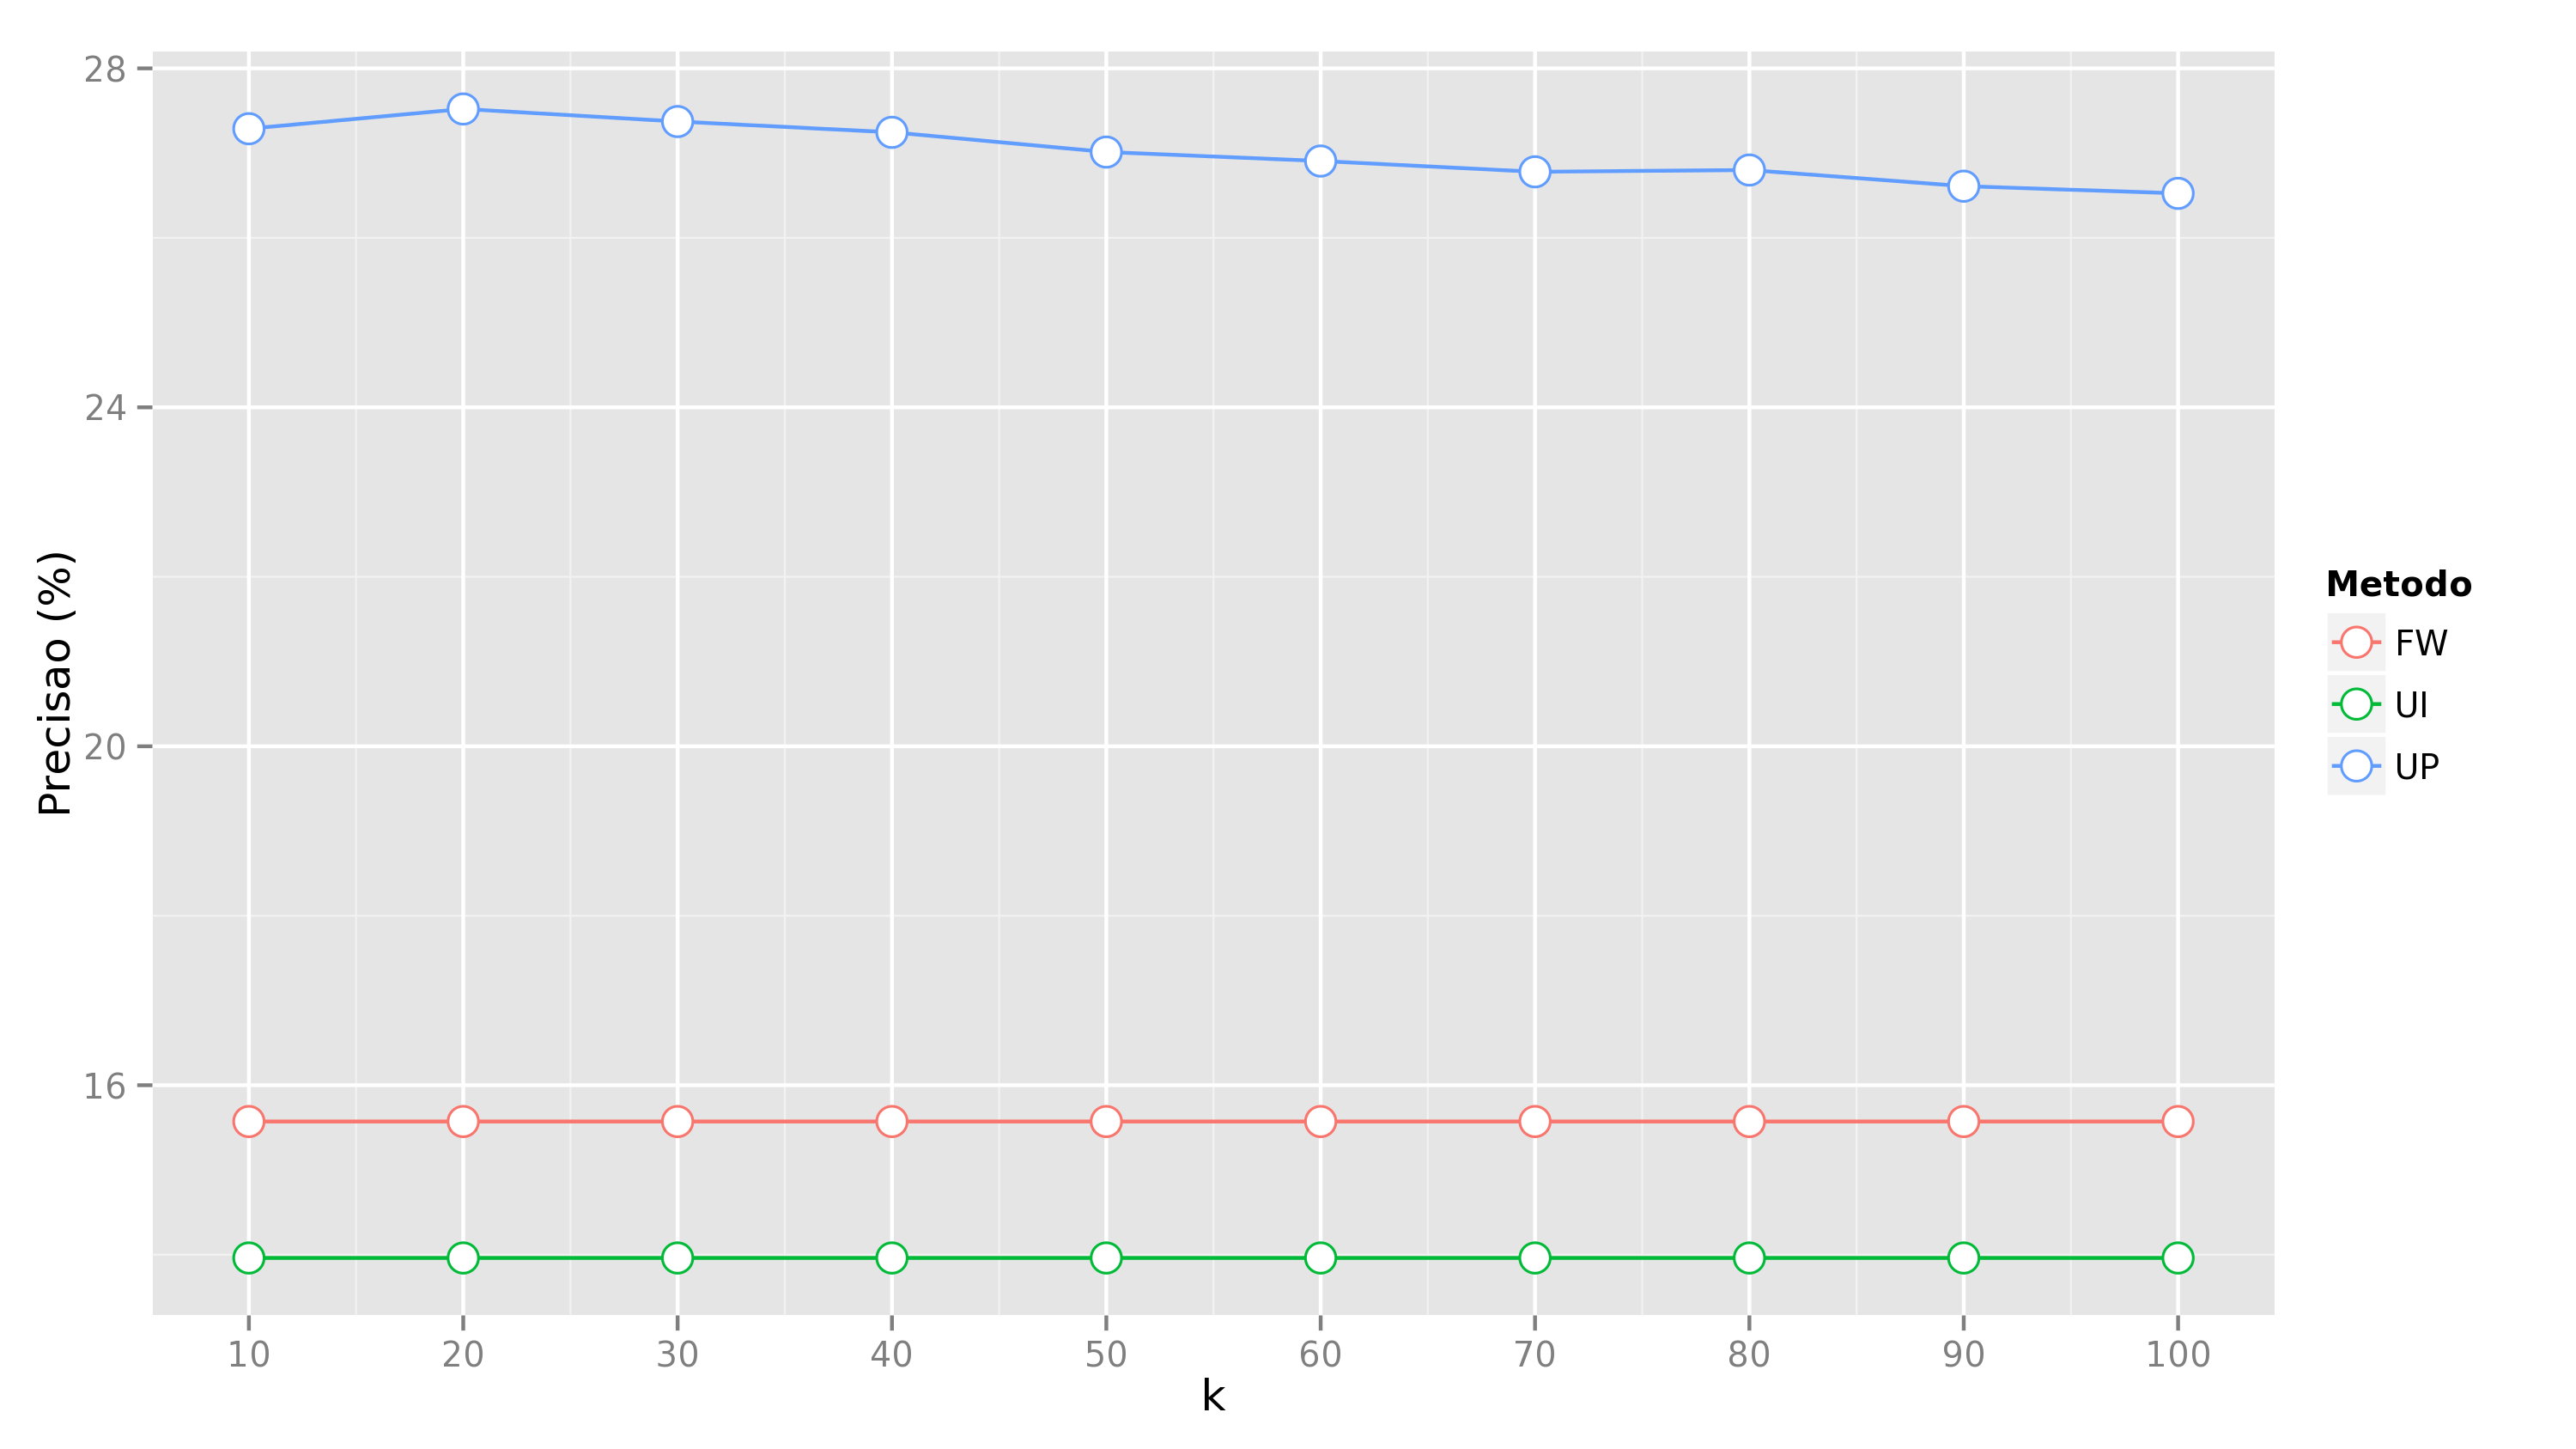
\includegraphics[width=1\textwidth]{img/precision_k}
    \end{center}
    \label{fig:precision_k}
    \caption{Precisão em função do número de vizinhos mais próximos $k$}
\end{figure}


\begin{figure}[htp]
    \begin{center}
    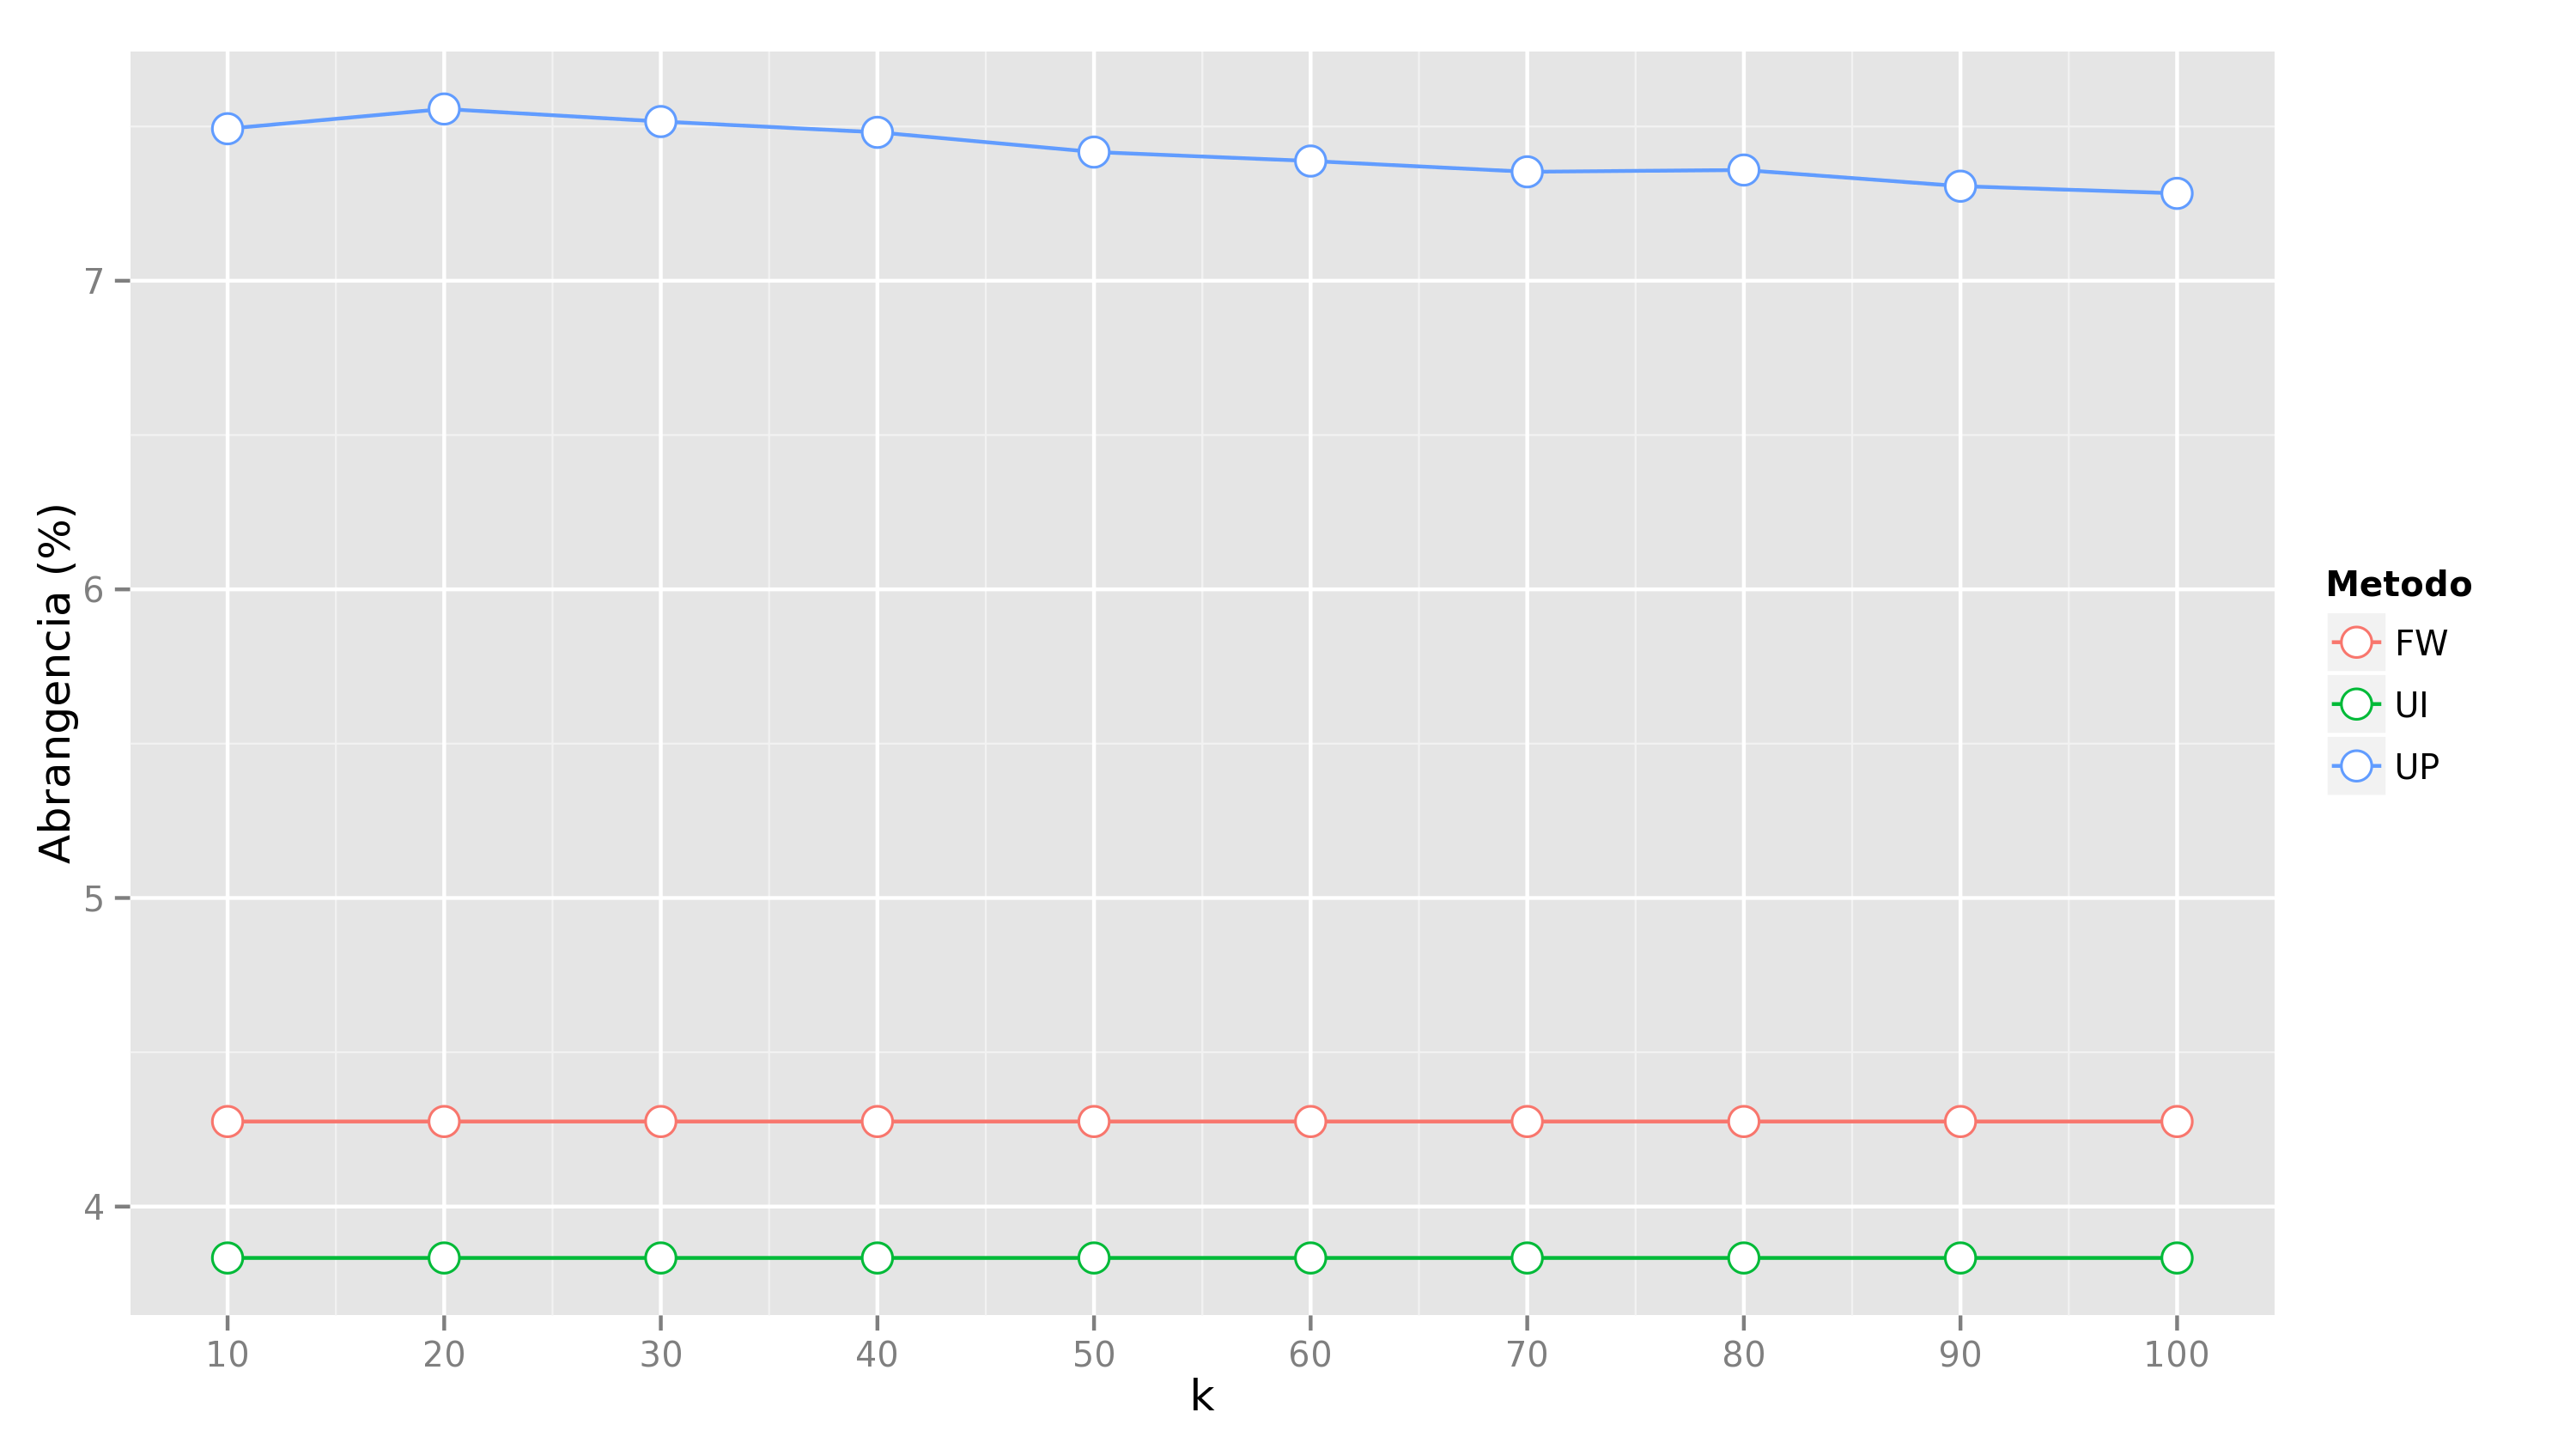
\includegraphics[width=1\textwidth]{img/recall_k}
    \end{center}
    \label{fig:recall_k}
    \caption{Abrangência em função do número de vizinhos mais próximos $k$}
\end{figure}

\begin{figure}[htp]
    \begin{center}
    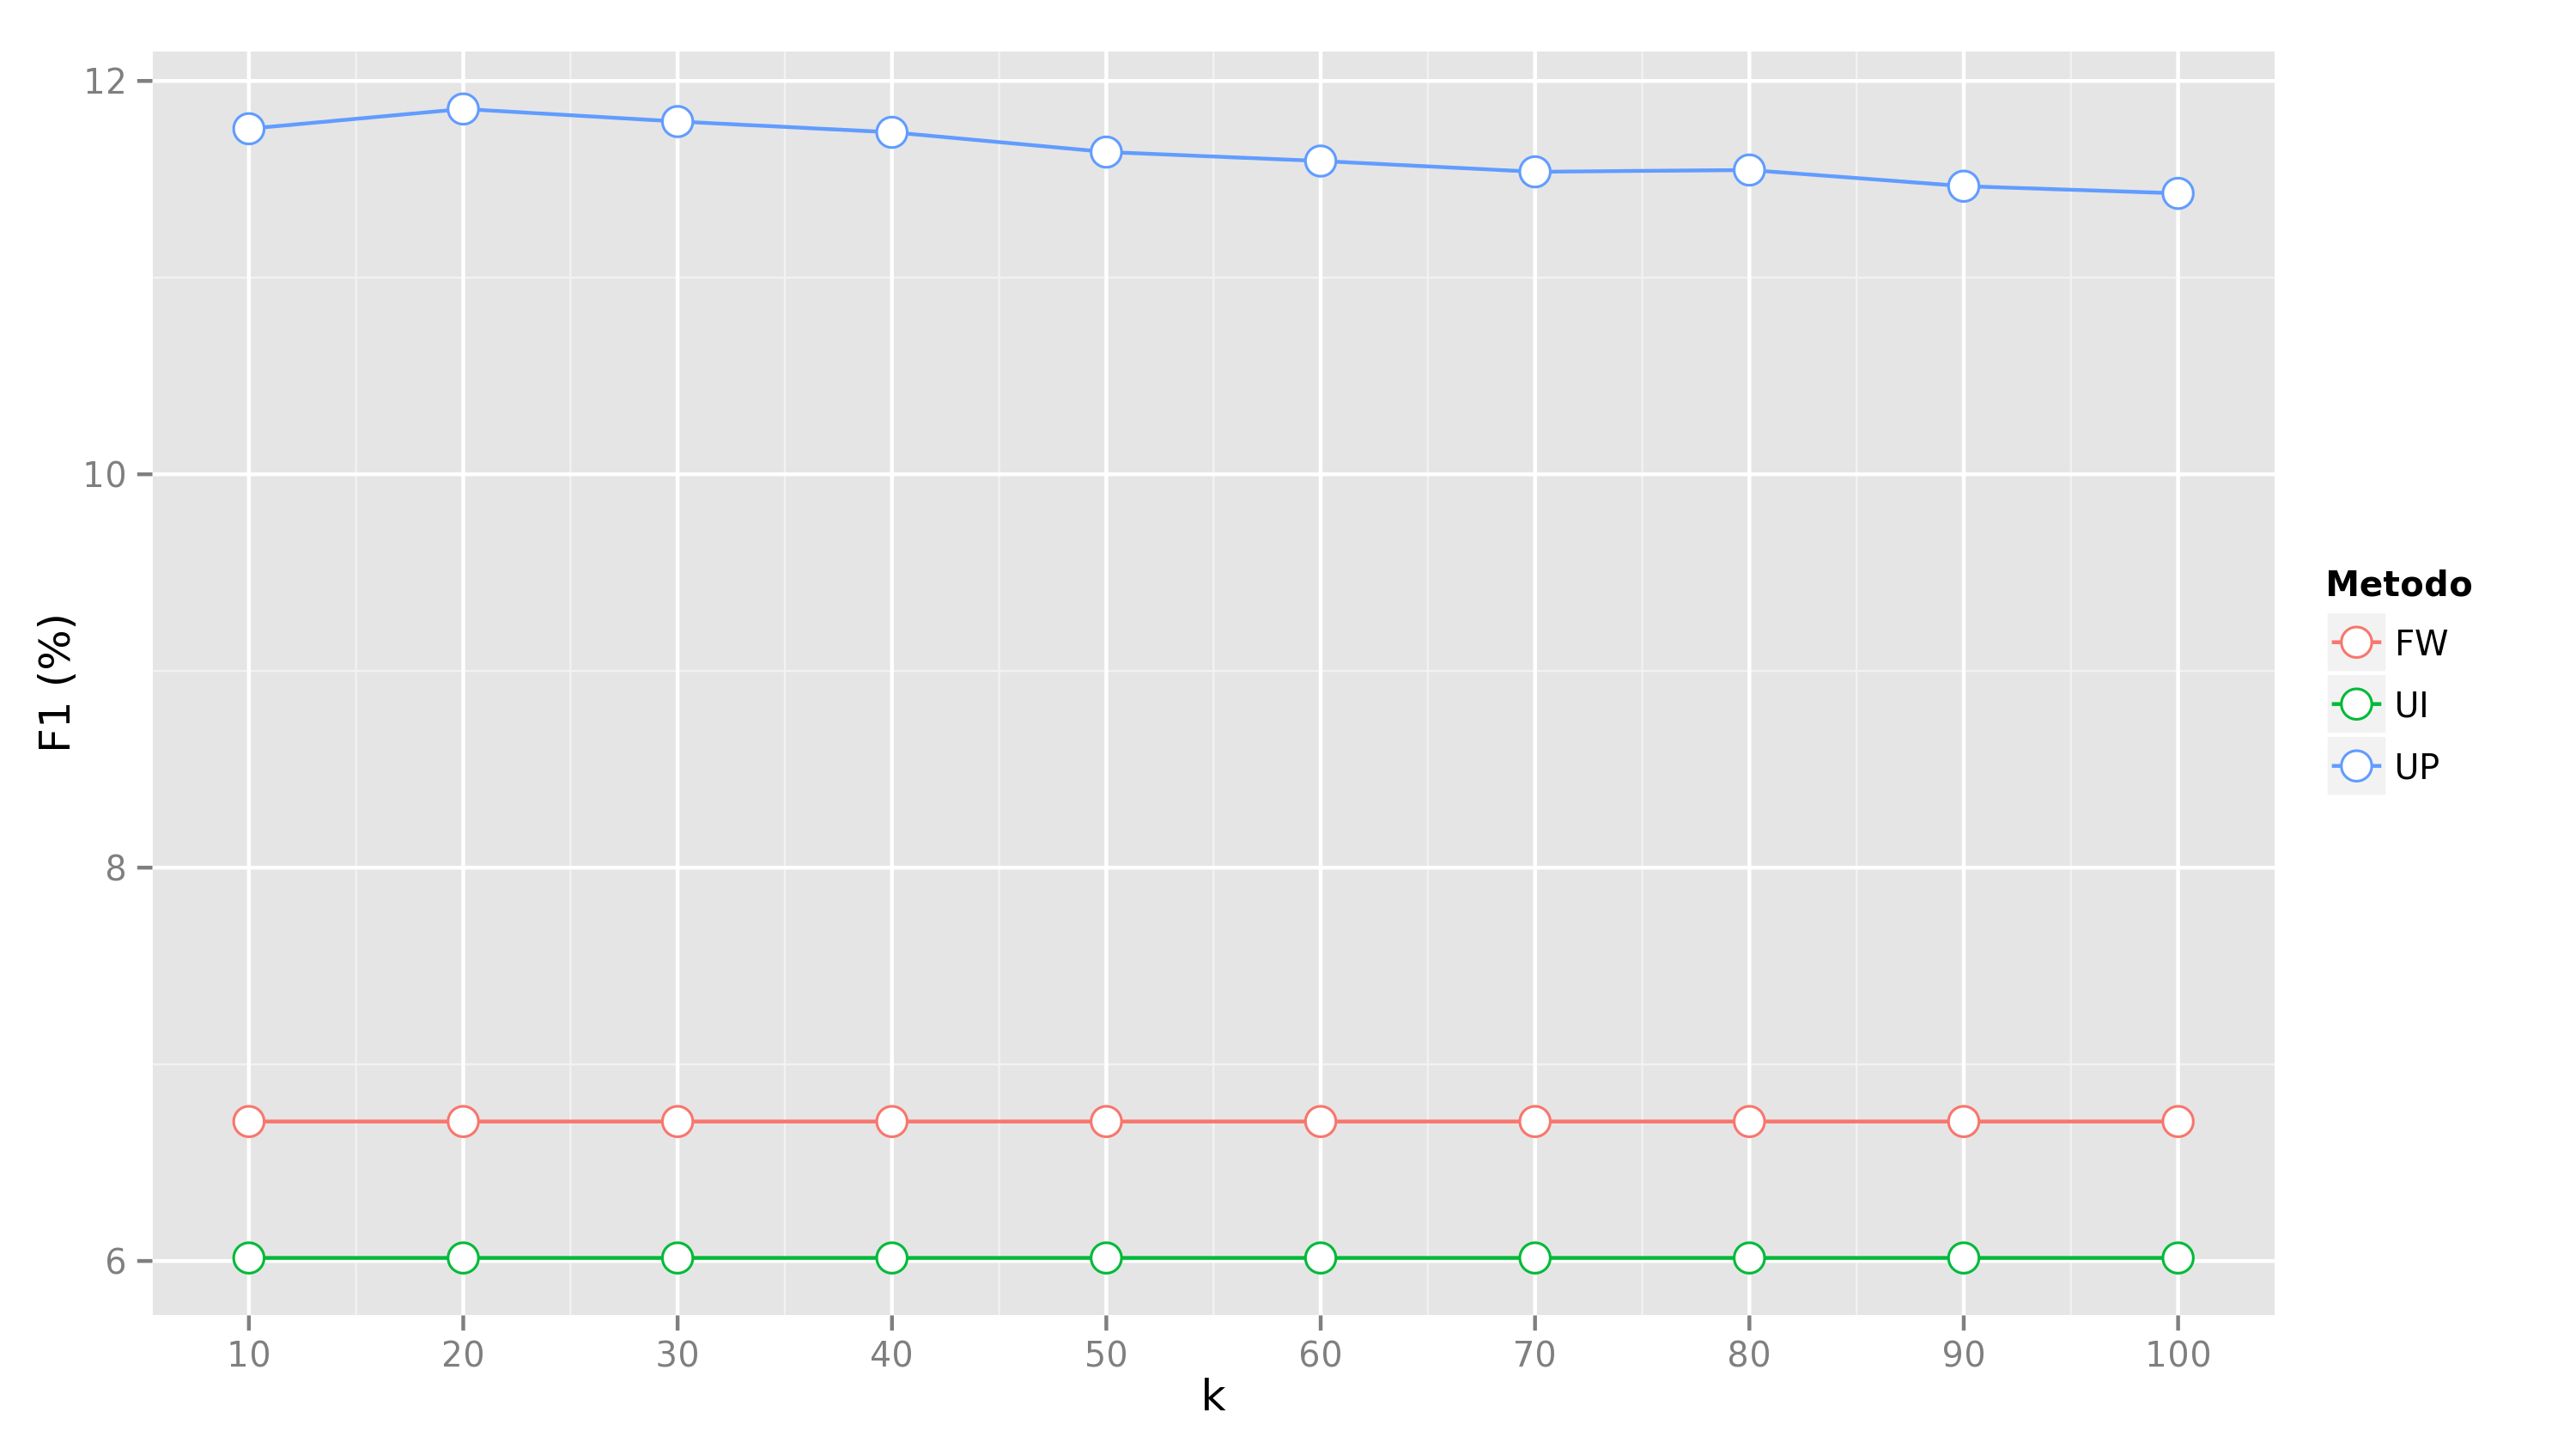
\includegraphics[width=1\textwidth]{img/F1_k}
    \end{center}
    \label{fig:F1_k}
    \caption{Medida $F_1$ em função do número de vizinhos mais próximos $k$}
\end{figure}

%\begin{figure}[htp]
    %\begin{center}
   % 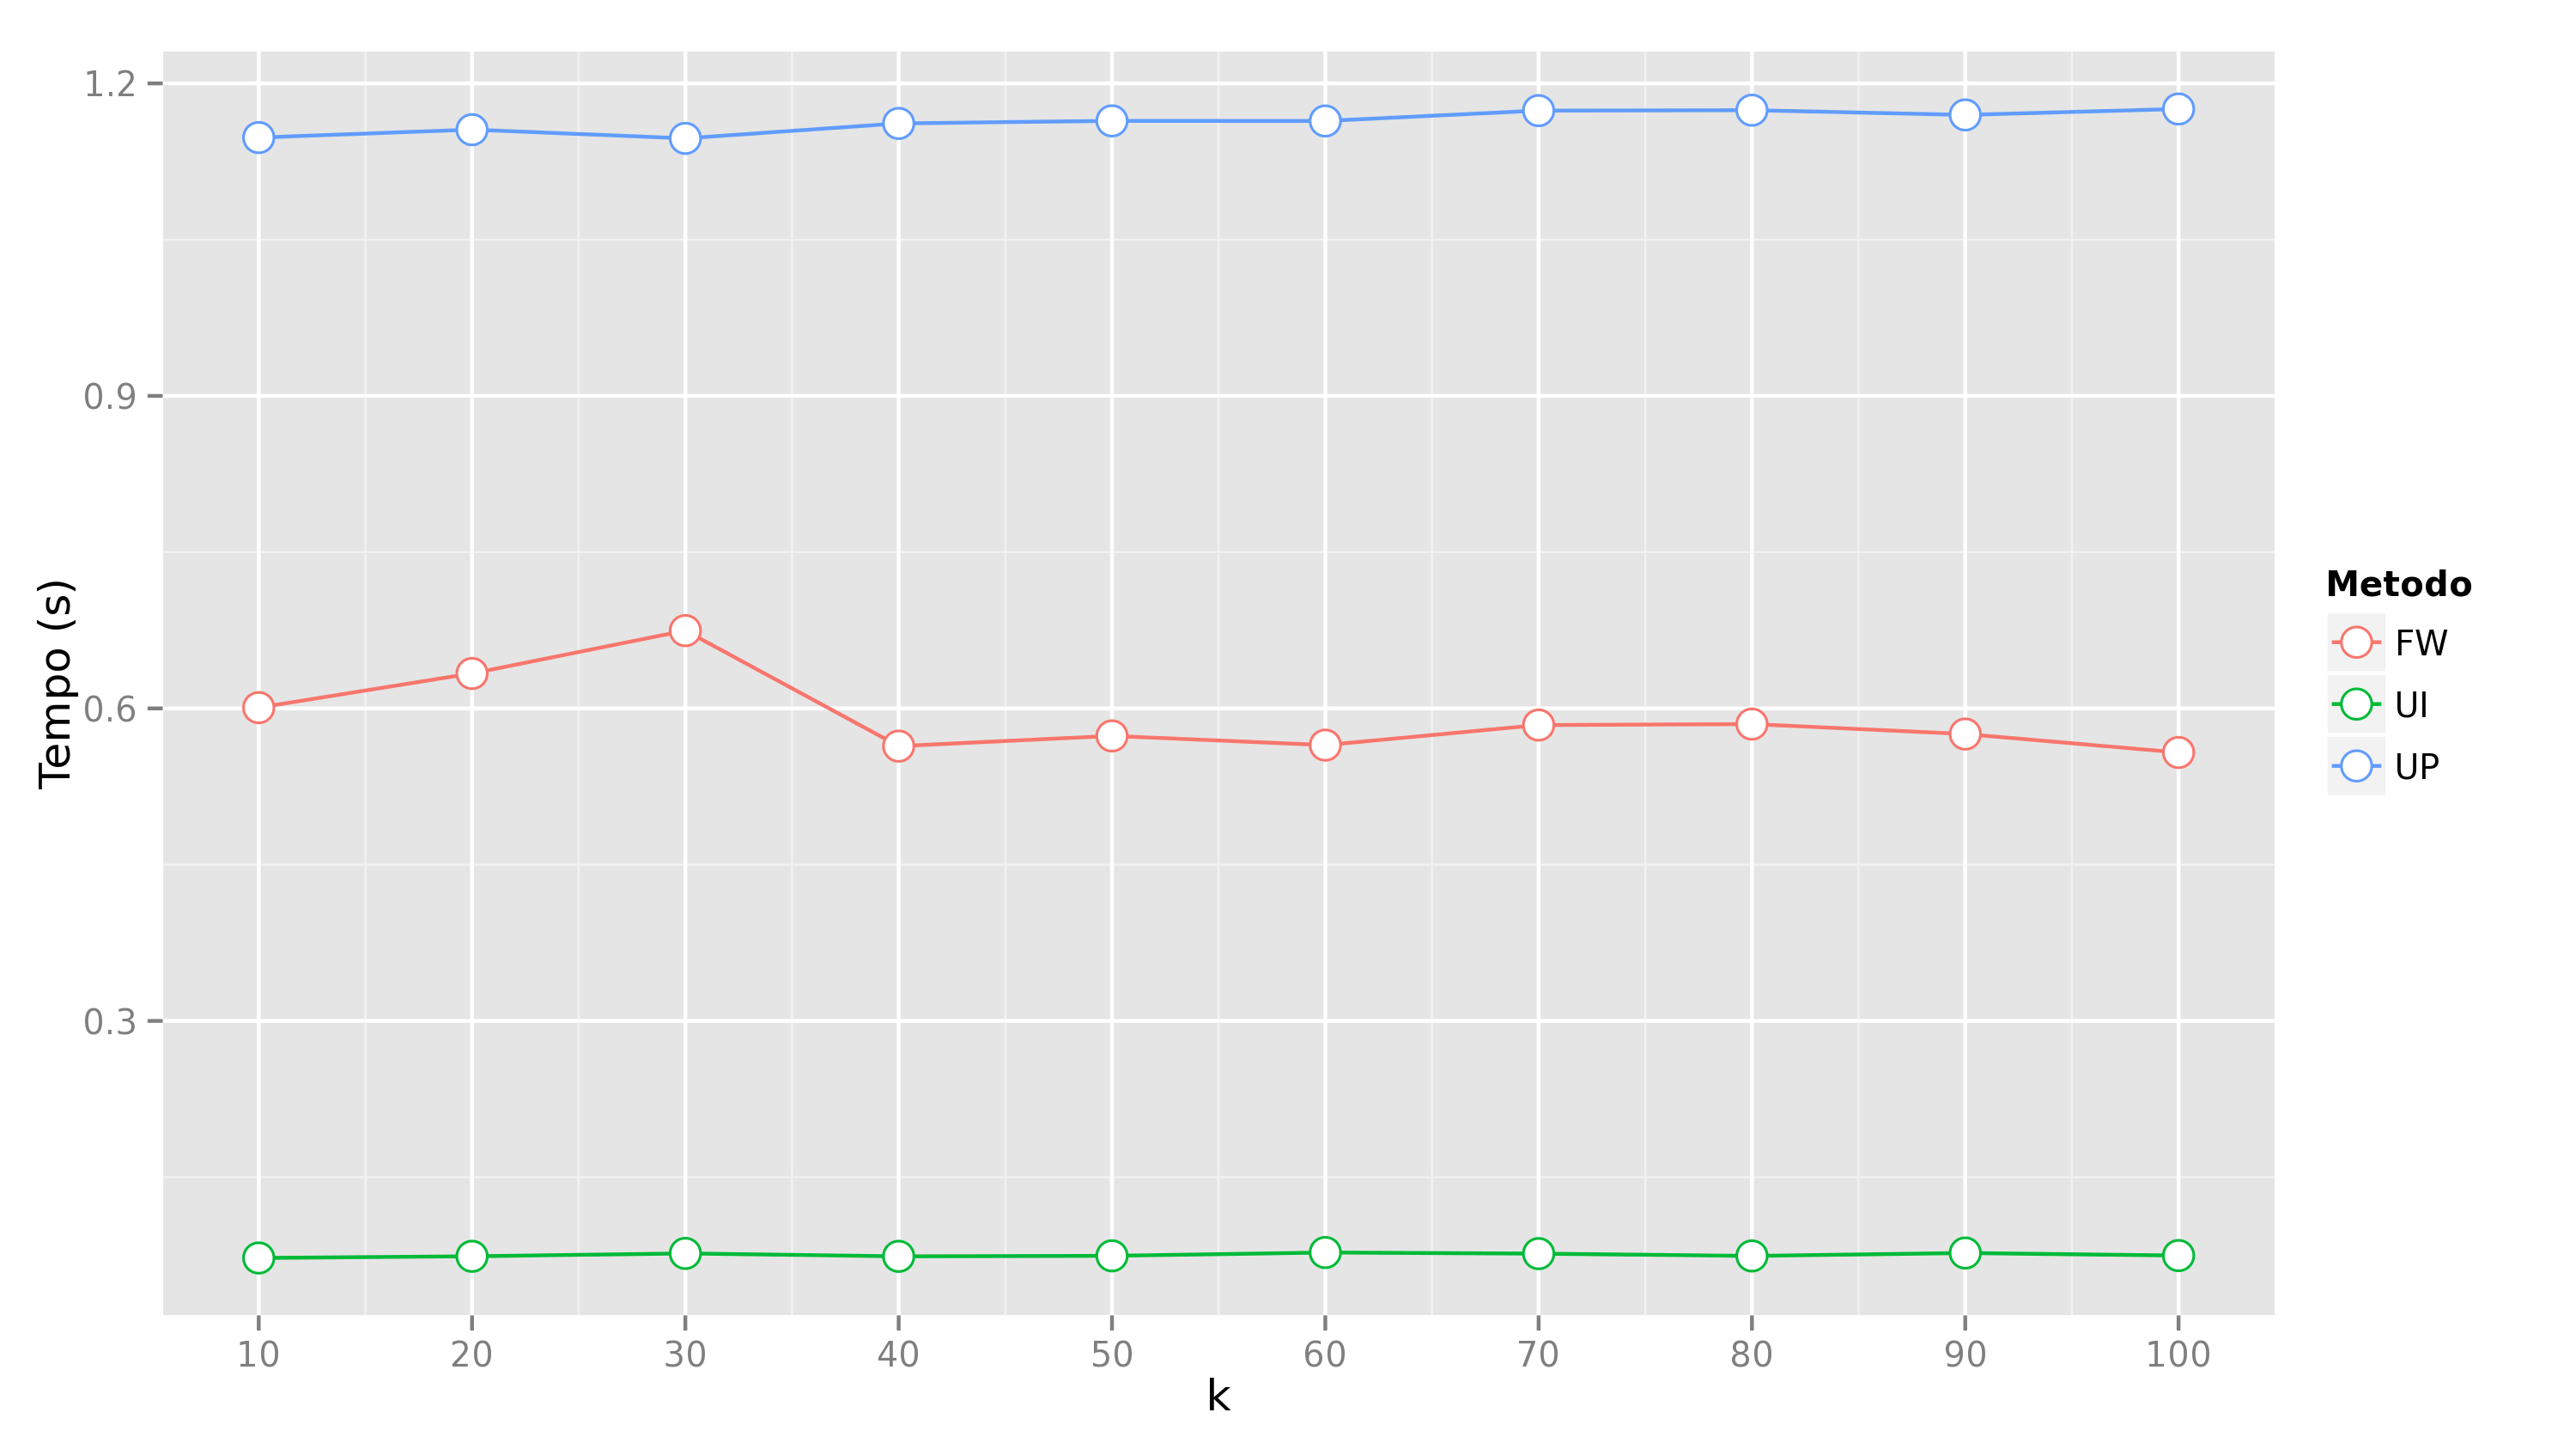
\includegraphics[width=1\textwidth]{img/time_k}
  %  \end{center}
 %   \label{fig:time_k}
%    \caption{Tempo de execução em função do número de vizinhos mais próximos $k$}
%\end{figure}

\section{Conjunto de atributos dos itens
 $\mathcal{F}$} % (fold)
\label{sec:conjunto_de_atributos_dos_itens_}


\section{Medida de distância entre atributos $d^f$} % (fold)
\label{sec:medida_de_dist_ncia_entre_atributos_}


\section{Pesos dos atributos $w_f$} % (fold)
\label{sec:pesos_dos_atributos_}

% section pesos_dos_atributos_ (end)

























\chapter[old]{old}
\label{chap:old}

\section{Primeira etapa do Trabalho de Conclusão de Curso} % (fold)
\label{sec:primeira_etapa_do_trabalho_de_conclus_o_de_curso}

% section primeira_etapa_do_trabalho_de_conclus_o_de_curso (end)
Os resultados da primeira etapa deste Trabalho de Conclusão de Curso, realizadas na disciplina PMR2500, foram principalmente a definição de necessidades, de parâmetros de sucesso e a elaboração de possíveis soluções. 

Definimos que a aquisição de dados seria feita a partir de uma base qualquer, que deveria alimentar o sistema por meio de arquivos de texto com valores separados por vírgulas (\texttt{.csv}).

A fim de facilitar o pré-processamento dos dados, estabelecemos que seriam necessários dois arquivos. Um deles deve conter a matriz de atributos $\mathbf{A}$ e o outro, a matriz de avaliações  $\mathbf{R}$. 

\begin{equation} 
\mathbf{A} = 
\begin{bmatrix} 
 a_{i_1 f_1} &  a_{i_1 f_2} &  a_{i_1 f_3}  & \dots   \\
 a_{i_2 f_1} &  a_{i_2 f_2} &  a_{i_2 f_3}  & \dots   \\
 a_{i_3 f_1} &  a_{i_3 f_2} &  a_{i_3 f_3}  & \dots  \\ 
 \vdots &  \vdots &  \vdots  & \ddots   \\
 \end{bmatrix}
\end{equation}


\begin{equation}
	  \mathbf{R} = 
\begin{bmatrix} 
  r_{u_1 i_1} &  r_{u_1 i_2} &  r_{u_1 i_3}  & \dots   \\
 r_{u_2 i_1} &  r_{u_2 i_2} &  r_{u_2 i_3}  & \dots   \\
 r_{u_3 i_1} &  r_{u_3 i_2} &  r_{u_3 i_3}  & \dots  \\ 
 \vdots &  \vdots &  \vdots  & \ddots   \\
\end{bmatrix}
\end{equation}

Em alguns bancos de dados relacionais, a tabela de avaliações também contém informações adicionais $\theta$, tais como método de pagamento, data da compra, data de entrega, etc., e é denominada matriz histórico de avaliações $\mathbf{H}$. Optamos, no nosso projeto, por não aceitar esse tipo de informação, e nem tampouco dados ligados a características de clientes (matriz $\mathbf{B}$). Para o emprego do sistema de recomendação em um e-commerce real, deve-se portanto efetuar ajustes no algoritmo a fim de tratar de particularidades envolvendo informações adicionais e arquivos suplementares.

\begin{equation} 
\mathbf{H} =
\begin{bmatrix} 
 r_{u_1 i_1} &  \theta_{h_1 1} &  \theta_{h_1 2} & \dots   \\
 r_{u_1 i_2} &  \theta_{h_2 1} &  \theta_{h_2 2} & \dots   \\
 r_{u i} &  \theta_{h 1} &  \theta_{h 2} & \dots   \\
 \vdots &  \vdots &  \vdots  & \ddots   \\
 \end{bmatrix} \\
\end{equation}

\begin{equation}
	\mathbf{B} = 
\begin{bmatrix} 
 b_{u_1 c_1} &  b_{u_1 c_2} &  b_{u_1 c_3}  & \dots   \\
 b_{u_2 c_1} &  b_{u_2 c_2} &  b_{u_2 c_3}  & \dots   \\
 b_{u_3 c_1} &  b_{u_3 c_2} &  b_{u_3 c_3}  & \dots  \\ 
 \vdots &  \vdots &  \vdots  & \ddots   \\
 \end{bmatrix}
\end{equation}

Uma vez determinada a forma de entrada de informações, definiram-se os conjuntos de dados que serão utilizados. O primeiro conjunto de dados abertos é proveniente do sistema de recomendações de filmes MovieLens (\url{http://movielens.umn.edu}). Nessa base de dados, o catálogo de filme faz o papel de catálogo de produtos, e o histórico de compras se refere à avaliação dos filmes feita por cada usuário. Outro conjunto de dados abertos é do website Internet Movie Database (IMDB). Na nossa análise, esses dois bancos poderão ser utilizado complementar ou independentemente.

Na primeira etapa do projeto, buscamos parcerias com e-commerces que estivessem dispostos a doar anonimamente seu banco de dados. Há ainda a possibilidade de utilizarmos uma terceira base, mas visto que as negociações ainda não foram concluídas, daremos prioridades aos conjuntos \textit{open source}.  

\section{Segunda etapa do Trabalho de Conclusão de Curso} % (fold)
\label{sec:segunda_etapa_do_trabalho_de_conclus_o_de_curso}

% section segunda_etapa_do_trabalho_de_conclus_o_de_curso (end)

A partir da síntese de soluções estabelecida na primeira etapa do projeto, implementamos os três algoritmos de recomendação e as medidas de recomendação na linguagem de programação estatística R. O código já está disponível para consulta através do endereço \url{https://github.com/aviggiano/tcc}.

Ainda na etapa de implementação, confirmamos a validade de cada um dos métodos aplicando-os nas matrizes-referência (Tabelas \ref{tab:rui_ref} e \ref{tab:aif_ref}). 

Em seguida, fizemos o tratamento das bases de dados, adequando-as ao formato de entrada especificado, e  iniciamos o processo de desenvolvimento do \textit{cross-validation}.

Para os trabalhos futuros, iremos realizar a validação cruzada e avaliar se os requisitos funcionais foram estabelecidos. Em seguida, procuraremos melhorar o sistema de recomendação a fim de torná-lo mais genérico. Buscaremos eliminar restrições quanto a entrada e saída de dados, de forma que elas sejam completamente arbitrárias. O objetivo é que o usuário possa informar ao sistema como é formado sua base, e que todo o tratamento preliminar seja feito automaticamente. 

Caso haja tempo, trabalharemos também na construção de um \textit{driver} que possibilite a conexão entre o sistema de recomendação e um banco de dados SQL, sem que seja necessária a etapa intermediária de arquivos \texttt{csv} para aquisição de dados. Planejamos elaborar um \textit{website} para o sistema de recomendação e exportar toda a lógica para um servidor dedicado. Outra melhoria desejada é a reconstrução dos métodos na linguagem de programação C, a fim de melhorar a performance computacional. Dessa forma, o serviço de ``sistema de recomendação nas nuvens'' estaria completo e poderia ser utilizado por e-commerces reais.
%%!TEX root = index.tex
\chapter[Cronograma]{Cronograma}
\label{chap:cronograma}

O cronograma de atividades da dupla busca seguir o cronograma proposto pela banca avaliadora dos trabalhos de conclusão de curso, estando sempre à frente das entregas em pelo menos uma semana. Dessa maneira, é possível apresentar a entrega antecipadamente ao orientador e falar sobre possíveis mudanças ou correções.

Além disso, semanalmente os alunos se reunem com o orientador a fim de conversar sobre o andamento do projeto, apresentar-lhe o esboço dos relatórios e discutir a implementação dos algoritmos. 

Para o segundo semestre, trabalharemos na implementação do sistema de recomendação já no período de férias escolares, para poder ter uma amostra funcional no início das aulas. Em seguida, daremos início ao relatório final em paralelo com os testes de performance do sistema de recomendação, e esperamos finalizar o projeto dentro do prazo estipulado.

O cronograma detalhado da dupla está descrito a seguir:

\begin{description}
 	\item[09/04] Análise do banco de dados e determinação das medidas de similaridade
 	\item[16/04] Esboço do relatório final
 	\item[23/04] Validação I do relatório final
 	\item[07/05] Validação II do relatório final
 	\item[14/05] Desenvolvimento dos Algoritmos de Recomendação 
 	\item[28/05] Validação III do relatório final
 	\item[04/06] Esboço do resumo final e da apresentação
 	\item[09/06] Validação do resumo final
 	\item[11/06] Validação da apresentação
 	\item[13/06] Ensaio da apresentação
 	\item[23/06] Apresentação para o orientador
 	\item[]
 	\item[09/07] Consolidação do Banco de Dados
 	\item[16/07] Programação de varredura do Banco de Dados
 	\item[23/07] Programação metodo proposto em \cite{symeonidis2007feature}
 	\item[30/07] Programação metodo proposto em \cite{debnath2008feature}
 	\item[13/08] Relatório de atividades de implementação
 	\item[27/08] Primeiros testes com o sistema (desvio de similaridade para uma base teste)
 	\item[03/09] Testes com o sistema (validação cruzada)
 	\item[24/09] Melhorias incrementais e relatório de atividades
 	\item[15/10] Relatório aprofundado de atividades
 	\item[05/11] Elaboração da apresentação e finalização dos relatórios
 	\item[12/11] Melhorias incrementais
 \end{description} 

\appendix
%!TEX root = index.tex
{\unnumbered
\begin{frame}[allowframebreaks]{Bibliografia}
\bibliography{../bibliografia}
\end{frame}}

\end{document} 
